\documentclass[twocolumn]{article}

%% Language and font encodings
\usepackage[english]{babel}
\usepackage[utf8x]{inputenc}
\usepackage[T1]{fontenc}

%% Sets page size and margins
\usepackage[a4paper,top=3cm,bottom=2cm,left=3cm,right=3cm,marginparwidth=1.75cm]{geometry}

%% Useful packages
\usepackage{amsmath}
\usepackage{graphicx}
\usepackage{float}
%\usepackage{gensymb} %make degree by $^{\circ}$
\usepackage{subcaption} %for subfigures
\usepackage[colorinlistoftodos]{todonotes}
\usepackage[colorlinks=true, allcolors=blue]{hyperref}
\usepackage[toc,page]{appendix}
\usepackage{titlesec}
\usepackage{wrapfig}
\usepackage{placeins}

\titleformat*{\section}{\LARGE}
\titleformat*{\subsection}{\normalsize\bfseries}
\titleformat*{\subsubsection}{\normalsize}
\titleformat*{\paragraph}{\small\bfseries}
%\titleformat*{\subparagraph}{\large\bfseries}

%% Set bibliography setup
\usepackage{natbib} 
\bibliographystyle{apalike}

%% Header
\title{Investigating water stratification during the Messinian Salinity Crisis with an advection-diffusion box model}
\author{Timo Millenaar}

\begin{document}


\twocolumn[
  \begin{@twocolumnfalse}
    \maketitle
    \begin{abstract}
    Vast deposits of evaporites are found below and around the present day Mediterranean sea. These evaporites originated from a period often referred to as the Messinian Salinity Crisis (MSC). Whether the bulk of these Messinian deposits originated from a deep or shallow sea is still a matter of debate. In this paper, a linear diffusion advection box model is developed and used as a first order approximation to investigate under what conditions a dense brine may be formed at the bottom of the deep basin as a result of exchanging flow between the deep basin and a shallow marginal basin. In an attempt to verify the viability of this possibility, scenarios are sought in which dense and saline water in the marginal basin could flow to the deep basin and sink as a consequence of its high density. Two scenarios are found in which it may be possible to create a dense brine at the bottom of the deep basin. In one scenario, an extra shallow marginal basin combined with a high background diffusion was able to sufficiently distribute the high salinity in summer throughout the marginal basin. The second scenario that showed to be successful is one with a net evaporation over the year, resulting in increasing salinity in both basins. The high evaporation has more impact on the smaller marginal basin, increasing its salinity and therefore its density more quickly then that of the deep basin. 
    \vspace{0.5cm}
    \end{abstract}
  \end{@twocolumnfalse}
]

\section{Introduction}
\subsection{Models of the Messinian Salinity Crisis}
Below and around the present day Mediterranean sea, vast deposits of evaporites have been discovered and described \citep{hsu1972origin, krijgsman1999chronology, rouchy2006messinian, roveri2014messinian, garcia2018geochemical}. These evaporites were deposited during the Messinian in what is generally referred to as the Messinian Salinity Crisis (MSC). Marginal basins around the Mediterranean, some of which are now found well above sea level, generally contain selenitic gypsum deposits \citep{garcia2018geochemical}. These marginal basins were of shallow depth at the time of deposition, generally not surpassing 200m. In Sicily, a succession containing Halite is thought to be deposited in a basin of intermediate depth (up to a kilometre). In deeper Mediterranean basins, evaporite deposits up to two kilometres thick are found. In some locations, these deposits consist primarily of halite, while in others a gypsum-halite-gypsum trilogy is found \citep{roveri2014messinian}. The up to a kilometre thick halite deposit in this succession is often termed the 'Mobile Unit'. Of this Mobile Unit, only the top few metres have been drilled \citep{hsu1972origin}. This lack of data on the deeper halite deposits leaves room for speculation about its depositional setting. Several conceptual models have been proposed to explain the origin of, and developments during the MSC, the most prominent of which can can be grouped into the following categories:\\

1) The 'desiccated, deep-basin model', initially proposed by \cite{hsu1972origin}, in a paper where drill cores taken from the top of the deep basin evaporites were discussed. These sediments were interpreted to be shallow water deposits. They proposed that a basin with a depth near that of the current Mediterranean was closed off from the world's oceans to subsequently desiccate, giving rise to extensive playa lakes that resided well below global sea level. 

2) The 'shallow-water, shallow-basin model', proposed by \cite{nesteroff1973mineralogy}, based on the similar interpretation to that of \cite{hsu1972origin}, that sediments in the deeper parts of the basin are of shallow water origin. Since these shallow water evaporites were deposited both in the deep basins as well as in the shallow marginal basins, they reasoned that the deep basin floor must have been brought up to a depth of 200-500 metres by vertical tectonic movements. Then a period followed where a cyclic opening and closing of the gateway would allow ocean waters to enter the basin during which evaporites were deposited. Finally these vertical tectonic movements would have brought the basin floor down to its present depth.

3) The 'shallow-water, deep-basin model', described by \cite{rouchy2006messinian}, where limited inflow through narrow or shallow straits, combined with high evaporation, kept the water from fully filling the basins. This resulted, episodically, in shallow brine seas where evaporites were deposited. 

4) The 'deep-water, deep-basin model', described by \cite{schmalz1969deep}, where dense, saline surface water was formed as a result of evaporation. As the dense water sank, it cooled, increasing its density further until it arrived at the basin floor. There it would, due to its high density, only be replaced if even denser water were to take its place. This stagnation of a dense brine would result in the precipitation of evaporites there.\\

With the recovery of drill cores from the deeper parts of the Mediterranean \citep{hsu1972origin}, the 'deep-water, deep basin model' lost support as the recovered sediments were interpreted to be deposited in shallow water conditions. A point of caution however, also noted by \cite{nesteroff1973mineralogy}, is that the deep basin cores represent only the terminal part of the MSC, since only the top few metres of the evaporite succession were drilled. The 'shallow-water, shallow-basin model' was not widely adopted, given the lack of a mechanism capable of inducing these large vertical movements in the Mediterranean, especially in the time span of a few million years. The 'desiccated, deep-basin model' became the widely accepted model. 
Later on, a model describing the relation between the marginal and deeper basins was proposed by \cite{rouchy2006messinian}. In this model the deepest parts of the basin are, depending on the relative sea level and the size of the gateways, either filled with deep water or with a brine sea. Evaporite deposition shifts, in this model, form one basin to another. This shift is, however, in contradiction with the findings of \cite{krijgsman2002onset}, who showed that the onset of the MSC was synchronous across the Mediterranean. 
More recent research questioned the interpretations concerning shallow water deposition, suggesting that the data was either inconclusive or could even be indicative of a deep water setting \citep{hardie2004did, roveri2001mediterranean}. On the basis of this, and the termination of erosional surfaces towards the deeper parts of the Mediterranean, \cite{roveri2014messinian} argued that deep water conditions may have persisted throughout the MSC. 
A variation of the 'deep-water, deep-basin model' was proposed by \cite{garcia2018geochemical}, where geochemical indicators in evaporites were examined. These indicated that the Mediterranean was highly stratified, with high salinity and dense, anoxic bottom waters. This led them to propose a variant of the 'deep-water, deep-basin model' where deposition of the marginal gypsum would be synchronous with the deposition of halite from a dense brine in the deeper parts of the Mediterranean. In order to investigate the plausibility of the formation of a deep brine during the MSC, an analogue is made between the present day Dead Sea and the MSC. This analogy will be tested using a linear diffusion-advection box model.

\subsection{The Dead Sea as reference}
The Dead Sea is a present day land-locked, hypersaline basin. The physical processes in this basin are modeled and tested against measurements by \cite{Heiden2017Application}.

\subsubsection{Vertical stratification in the Dead Sea}
\label{sect:Dead_Sea_model}
 Before 1978, the basin was stratified and did not mix. The top of the basin contained a warm and fresh epilimnion. Below that, a cooler and more saline hypolimnion resided. Increasing irrigation combined with a changing climate lead to a steady decrease in fresh water runoff. In 1978, a threshold was reached where the density distribution of the water column became unstable. Since then, the water column undergoes vertical mixing during winter, resulting in a holomictic situation during winter. \cite{Heiden2017Application} used a linear diffusion model to replicate this annual mixing pattern. From this study, a conceptual model describing the annual mixing was formulated. In this model, as both the temperature and salinity of the epilimnion increase during summer, the water column remains stable since the high temperature of the epilimnion keeps it more buoyant then the hypolimnion. In this scenario, the epilimnion can be more saline then the hypolimnion, but still be stable. As the epilimnion cools however, it remains more saline then the hypolimnion and the density of the epilimnion increases until the water column becomes unstable and mixing occurs. 
 
\subsubsection{Applicability of the Dead Sea model to the MSC}
While a permanent inflow of solutes form a parent ocean is required to explain the vast volume of evaporite deposits \citep{garcia2018geochemical}, a connection the likes of which is absent from the present day Dead Sea, the Dead Sea model will be used as a first order analogue for the MSC. In both systems, we are dealing with a (largely) isolated, hypersaline basin where evaporite deposition is partially controlled by climatic oscillations \citep{manzi2012high}. Among present day hyper saline basins, the Dead Sea is one of the most prominent, making it one of the better candidates to study hyper saline lake dynamics. This study adds to the model of \cite{Heiden2017Application} to apply it to a marginal basin - deep basin configuration of the MSC.

\subsection{Marginal basins as agent for stratification}
\label{uitleg_conceptuele_model}
The model of a stratified Messinian Mediterranean as presented by \cite{garcia2018geochemical}, illustrated in their Figure 12, contains a dense, anoxic brine at the bottom, normal marine waters at the top and a gypsum saturated layer in between. This does not combine well with the holomictic Dead Sea model, where the top layer is generally the most saline part of the column. A possible solution to bring these scenarios together, inspired by \cite{waahlin2006entraining}, is to involve the marginal basins of the Mediterranean. Water from the top of the main Mediterranean basin could flow into the marginal basins. Here, evaporation will increase the salinity of this water. As the water cools in the fall, like in the Dead Sea model, the water column in the marginal basin would mix. This would then result in an increased density of the water at the bottom of the marginal basin. While this effect would likely also take place in the deeper Mediterranean column, the increased density of the bottom water would be more pronounced in the marginal basins, precisely because of their shallower depth. If the density in the bottom of the marginal basin is higher than that in the bottom of the deeper basin, water could, due to buoyancy, flow from the marginal basin into the deeper parts of the main basin. There it would only be replaced by even denser water. This hypothesis resembles the 'Deep water, deep basin model' as described by \cite{schmalz1969deep}, but with marginal basins essentially acting as evaporative pools. 

%% In this study..
In this study, a linear diffusion-advection box model, consisting of a deep and a marginal basin is used as a first order approximation to investigate the possibility of stratification in the Mediterranean basin during the MSC. 

%\section*{Quotes}
%\subsection{Halite precipitation:}
%Halite  does  not begin to  precipitate  until  the  brine  has  been  enriched   about   tenfold    (density 1.215 $g/cm^3$), and  more  than  80  percent  of  the  available  sodium  chloride  has  been  precipitated before the first  of  the  highly  soluble  salts  appears  at  nearly one-hundredfold  enrichment  of  the brine (density  very  nearly  1.26  $g/cm^3$). \citep{schmalz1969deep}
%\subsection{Differences between T and S diffusion}
%Down-flowing warm,salty water loses heat but not salt to surrounding cold, fresh water, thereby becoming denser and accelerating its flow. 
%\citep{schmitt1994double}


%\subsection{deep water proof}
%Widespread evidences for deep-water conditions before and after the MSC have been provided since a long time as the presence of psychrospheric ostracodes and benthic foraminifers usually living at depths comprised between 1000 and 1300 m (Benson, 1973a,b, 1978; Cita, 1973; Sprovieri et al., 1996a,b, 1999; Sgarrella et al., 1997). (...) Shallower conditions existed in some peripheral subbasins espe-cially on the northern margin. In contrast, there are huge differences between the sedimentary succession of the deeper areas of the Sicilian basin (central salt trough,area of Gibliscemi-Falconara) and those of the marginal basins (Fig. 4).
%From \citep{rouchy2006messinian}


%\subsection*{Stage 1}
%"They suggest that vertically-oriented selenites formed in moderately shallow marginal basins whereas the absence of oxygen prevented gypsum precipitation in deeper stratified areas." ... \linebreak "Organic-rich, barren shale and carbonate sediments deposited in the deeper parts of the Messinian marginal basins (...) suggest that gypsum saturation was not achieved there probably because of brine stratification and bacterial reduction of sulfate (Roveriet al., 2014a)." (stage 1) - \citep{garcia2018geochemical}


\section{Methods}
\subsection{Model setup and boundary conditions}
\subsubsection{The box model}
%%Introduce: 2 columns, diff, adv, SS, flowdepth
In order to investigate the influence of a shallow marginal basin on the conditions at which stratification could occur in a deep water basin, a box model was created. The box model expands on the linear diffusion code as used by \cite{Heiden2017Application}. In this box model, the two basins are each represented by a vertical column. For each of these columns, diffusivity and advection calculations are solved for both temperature and salinity. From these, the density is inferred. The top nodes of the two columns are connected via the source-sink term. The number of connected nodes can be varied. When the bottom nodes of the marginal basin column are denser then those at the bottom of the deep basin, flow is initiated from the bottom of the marginal basin to that of the deep basin. At this time, flow from the top of the deep basin to that of the marginal basin is also initiated, as is the advection within the columns. Advection goes up in the main basin and down in the marginal basin.

\subsubsection{Boundary conditions}
\label{sect:boundary_conditions}
%%Introduce: forcing, ramp
Initially, the temperature and salinity in each entire column are set to a user modifiable value, resulting in straight vertical profiles. A flux on the top node is then initiated. This flux is sinusoidal and is linearly proportional to the inverse of the diffusivity in the top two nodes. The sinusoidal flux for salinity can be assigned an above zero mean, resulting in net evaporation. The bottom node is not subject to any boundary conditions but is determined based on the node above it. At first, mixing, source-sink and advection are not active in the model.
There are two types of forcing in the model, a heat flux on the temperature and an evaporative flux on the salinity. The former is dependent on the surface water density and the heat capacity, the latter is dependent on the salinity of the surface water. Both are sine functions with a period of a year that affect only the top node.
During the first four years, the amplitude of the forcing will be increased from zero to 100$\%$, after which the amplitude will remain 100$\%$. After the first ten years, mixing, source-sink and advection will be turned on. I will refer to this ten year period as the spin-up period and it ranges from April year 0 until April year 10. Most scenarios in this research contain a marginal basin of 150m, for most marginal basins were shallower then 200m. While the deep basins are often over two kilometres deep, the scenarios in this model generally contain a deep basin of a mere 800m, for this reduces run time while preserving the general outcome of the model. %An example of the forcing used in the models on both the temperature and salinity is shown in figure \todo{add fig showing evap and heat flux}. 

%%Diffusion & FTCS
\subsection{Diffusion discretization}
The principal diffusion equation for a diffusive physical quantity (Q) in differential form, with advection and source sink is shown in equation \ref{eq:diff_original}.
\begin{equation}
    S = \frac{\delta Q}{\delta t} + w\frac{\delta Q}{\delta z} - D\frac{\delta^2 Q}{\delta z^2}
\label{eq:diff_original}
\end{equation}
Where \textbf{w} is the advection velocity in $m s^{-1}$, \textbf{D} is the diffusivity in $ms^{-1}$, $\Delta$\textbf{t} is the incremental timestep in $s$, $\Delta$\textbf{z} is the spatial increment in $m$ and \textbf{S} is the source-sink term in $[Q]s^{-1}$.  
This is discretized to equation~\ref{eq:FTCS}, formulated after the explicit Forward Time Central Space (FTCS) method as described in \cite{slingerland2011mathematical} p. 143.

\begin{equation}
\begin{split}
    S& =\frac{Q^{n+1}_i-Q^n_i}{\Delta t} + w\frac{ Q^n_{i+1}-Q^n_{i-1}}{2 \Delta z} -\\
		&D\frac{Q^n_{i-1} -2Q^n_{i}+Q^n_{i+1}}{\big( \Delta z \big)^2} 
\end{split}
\label{eq:FTCS}
\end{equation}

\noindent Here, $Q^n_i$ refers to the value of a diffusive physical quantity (Q) for time step \textit{n} at depth \textit{i}. Rewriting equation \ref{eq:FTCS} yields the desired diffusive physical quantity (Q) for the following timestep at depth \textit{i}, $Q^{n+1}_i$ as shown in equation \ref{eq:FTCS_rewritten}.

\begin{equation}
\begin{split}
    Q^{n+1}_i& = Q^n_i-\frac{w \Delta t}{2 \Delta z} \Big( Q^n_{i+1}-Q^n_{i-1} \Big) + \\
		&\frac{D \Delta t}{\big( \Delta z \big)^2} \Big( Q^n_{i-1}-2Q^n_{i}+Q^n_{i+1} \Big) + S \Delta t
\end{split}
\label{eq:FTCS_rewritten}
\end{equation}

\noindent This method of discretization does bring with it the following conditions:
\begin{equation}
    \Delta t \leq \frac{\Delta x^2}{2D} \qquad \text{and} \qquad \Delta t \leq \frac{2D}{w^2}
\label{eq:FCTS_limits}
\end{equation}

\noindent These conditions are used to dynamically adjust the size of the time step, according to 0.9 times the lowest $\Delta t$ between the various basins and criteria.

\subsection{Column stability}
\label{sect:stability_methods}
The model runs with a standard, minimal diffusivity that is always present and affects both entire columns. The diffusivity can be set individually for temperature and salinity. When part of the column is unstable, which can be the entire column, the unstable part is assigned a diffusivity orders of magnitudes higher to imitate the mixing of the column. This high diffusivity is assigned to both temperature and salinity.

In the Dead Sea model as described in \cite{Heiden2017Application}, the presence of an unstable column is determined by assessing if the top node is more dense then the one below it. For their model this is sufficient, but this creates the possibility of a dense water body at a certain depth that is considered stable by the model if there is less dense water above it. Therefore, an adaptation from \cite{Heiden2017Application} is required, where the bottom of the column is also checked for instability. Two methods are implemented, between which a choice has to be made before the run starts. In one method, the column is checked for instability both from the top down and from the bottom up. In the second method, any location is checked for instability and assigned an appropriate diffusivity. The consequences of these methods will be discussed in sections \ref{sect:transition} and \ref{sect:totals_problem}.

\subsection{Density calculations}
The density at a given node is determined using the equation of state as described in \cite{ivanov2002model}. They calculate the water density as a density anomaly from the reference density of 1e3 $kg$ $m^{-3}$. In this research, we will show the density as absolute values, therefore adding 1e3, resulting in equation \ref{eq:state}. Their values, determined for the Dead Sea, will be applied to the MSC in this research.
\begin{equation}
    \rho = \rho_{ref} + r_0 - \alpha T + \beta S
\label{eq:state}
\end{equation}
Where $r_0$ = -15.654, $\alpha$ = 0.4309 and $\beta$ = 0.936, as determined by \cite{ivanov2002model}. $\rho$ is the density in $kg$ $m^{-3}$, $\rho_{ref}$ is the reference density of 1e3 $kg$ $m^{-3}$, T is the temperature in $^{\circ} C$ and S is the salinity in $kg$ $m^{-3}$. 

% Fig SpinUp
%-------------------
\begin{figure*}
\centering
\hspace*{-1.2cm}
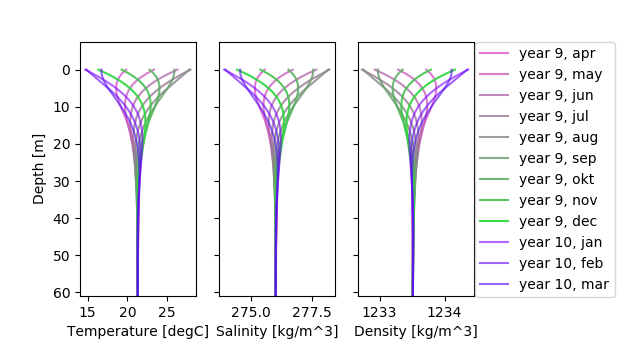
\includegraphics[width=1.05\textwidth,keepaspectratio]{SpinUp_year_9.png}
\caption{Last year of the 10-year Spin-Up period. This data was generated using an instability check in the top node instead of a whole column check for instability.}
\label{fig:SpinUp}
\end{figure*}

%%Boundary conditions

%%Dt and courant number

%%Density calculations

%%Volume determination, %%Source, Sink of Salt
\subsection{Source-sink and advection}
The volume of water that moves every time increment through the strait that connects the two basins, is determined by multiplying its width, depth and the lateral flow velocity through the strait. When the density of the bottom waters in the shallow basin is greater then that of the bottom waters in the deep basin, the flow of salt water from the shallow basin to the deep basin is initiated. The total amount of salt that is moved in this exchange is determined by multiplying the volume of water moved, with the salinity of the source. The impact this amount of transported salt has on a basins is dependent on the total volume of the basin in question. This exchange of salt is implemented through the source-sink term (\textbf{S}), as shown in equation~\ref{eq:FTCS}. \textbf{S} is calculated using equation~\ref{eq:Source-Sink} and is either positive or negative depending on whether it represents a sink or a source, respectively.
\begin{equation}
    S = \pm h_{source} \frac{ z_{strait} x_{strait} U_{lat} }{A_{sink} z_u} 
    \label{eq:Source-Sink}
\end{equation}
Where \textbf{h}$_{source}$ is the salinity of the source in $kg \hspace{0.8mm} m^{-3}$, \textbf{U}$_{lat}$ is the lateral flow velocity in $ms^{-1}$, $A_{sink}$ is the surface area of the sink basin in $m^2$, \textbf{z}$_u$ is the vertical extent of the flow in $m$ and \textbf{x}$_{strait}$ and \textbf{z}$_{strait}$ are the strait width and depth, respectively, in $m$.

The physical replacement of the bottom waters as a result of the lateral flow is captured in the advection, where advection is set to be upward in the deep basin and downward in the shallow basin. The value of the advection is equal to the volume of lateral flow per second, divided by the surface area of the basin in question. 

% Low salt_diff_amp
%
\begin{figure*}
%% subfig 1
\begin{subfigure}[h]{0.65\textwidth}
\centering
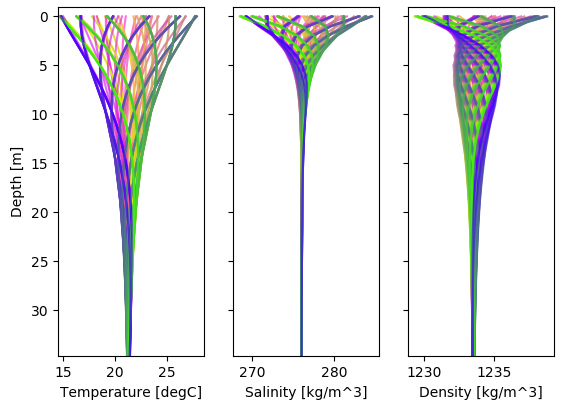
\includegraphics[width=\textwidth,keepaspectratio]{SDA-01_TDA-1_SpinUp.png}
\label{fig:}
\end{subfigure}\hfill
%% subfig 2
\begin{subfigure}[h]{0.25\textwidth}
\centering
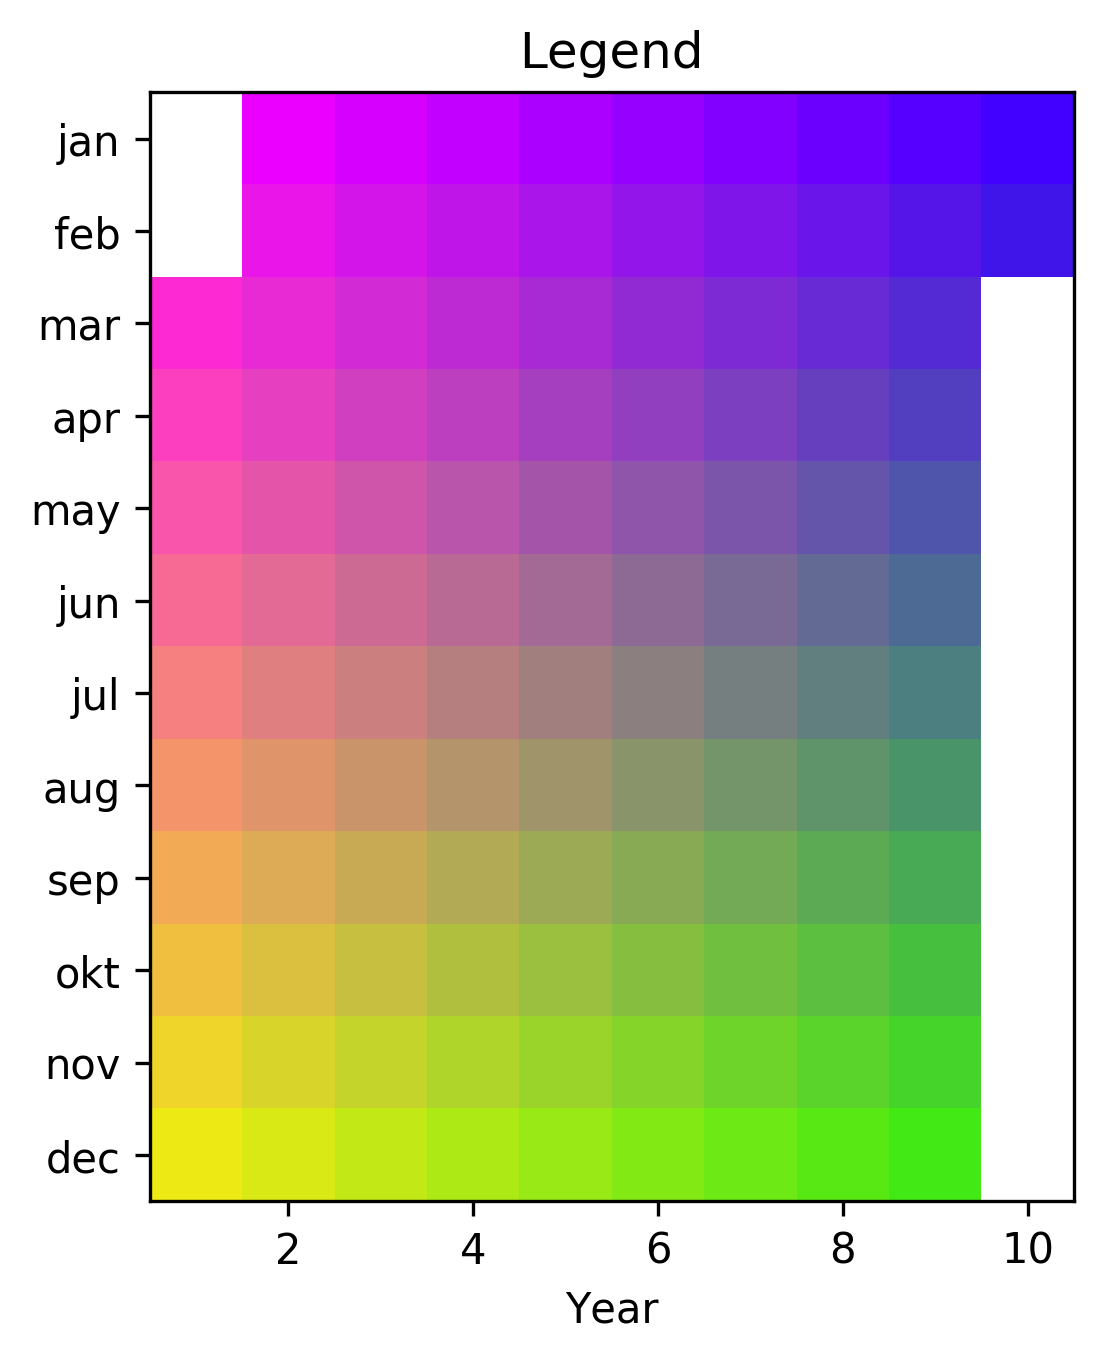
\includegraphics[width=\textwidth,keepaspectratio]{SDA-01_TDA-1_SpinUp_Legend.png}
\label{fig:}
\end{subfigure}\hfill
\caption{Spin-Up period with a salinity diffusivity one tenth of the temperature diffusivity. }
\label{fig:SpinUp_dencity_balance_example}
\end{figure*}



%%%%%%%%%%%%%%%%%%%%%%%%%%% Ref mod output

\section{Understanding the model}
In order to get a grasp on the basics of the model, some results from simplified scenarios are shown in this chapter. The basic boundary conditions are discussed as well as the relation between the temperature, salinity and density. All model cases that will be discussed are deviations from a standard model case of with the starting parameters are shown in appendix \ref{app:standard_parameters}.

\subsection{Forcing}
\subsubsection{Results}
The last year of the ramp period is shown in figure~\ref{fig:SpinUp}. Here, the amplitude of the forcing is at its maximum. Only the diffusion and the boundary conditions are active in this stage. 
The mean, as well as the amplitude of the forcing differ between the temperature and the salinity, but their general shape is identical. Both the temperature and salinity of the surface water increase from march until June and decrease from September until December. 

\subsubsection{Discussion}
During the ramp period, the temperature, salinity and density profiles show a symmetrical overall shape of the plot (see figure~\ref{fig:SpinUp}). This shape follows from the perfectly sinusoidal cyclicity of the forcing that is centered around zero. Below about forty metres there is no influence of the forcing, for the background diffusion is not quick enough to reach that depth within a year. 

The lower diffusivity of the salinity compared to that of the temperature, has two significant consequences. The first of these is the reduced depth to which the salinity forcing can penetrate within a given year. The second consequence is in the dependence of the forcing on the diffusivity in the model. Lower diffusivity results in higher forcing on the salinity, as mentioned in section \ref{sect:boundary_conditions}. A higher forcing, results in a higher amplitude in the salinity values. This means that, during winter, the surface water is less saline than for example that in figure \ref{fig:SpinUp}, resulting in a stable density distribution during winter and a regular linear relation between the density and the temperature and salinity. Since this effect only penetrates the water column for the first few metres, deeper in the column the temperature has more impact and the inverse balance of the density curve as seen in figure \ref{fig:SpinUp} is restored. This can be deduced from the equation of state as well (equation \ref{eq:state}), where the density decreases in a given location if $\alpha T$ increases more rapidly then $\beta S$ or $\beta S$ decreases more rapidly then $\alpha T$. The latter is the case in figure \ref{fig:SpinUp_dencity_balance_example}, where the value of $\beta S$ decreases significantly faster with depth then $\alpha T$. If the amplitude of evaporation forcing is significantly higher than the amplitude of the heat flux forcing, the salinity of the water will control the density profile. If that is the case, and assuming there is no net evaporation, the surface water lacks the salinity to become dense enough during winter to become unstable, while the water becomes so saline during summer that the water column becomes unstable, despite its high temperature.
 
 % Fig Transition
%-------------------
\begin{figure*}
\centering
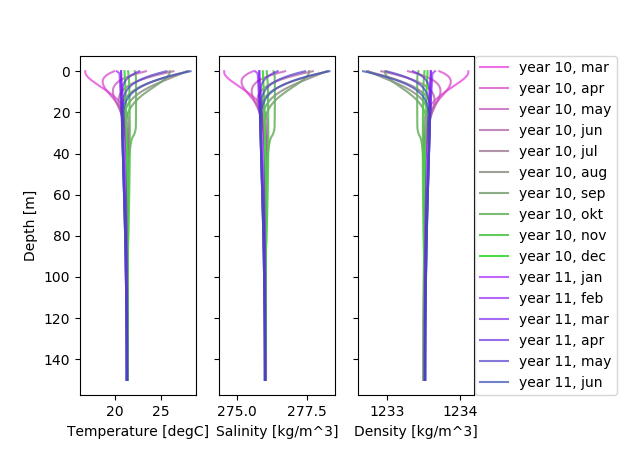
\includegraphics[width=0.9\textwidth,keepaspectratio]{Transition.png}
\caption{The transition from the Spin-Up period. The possibility of mixing is activated in April. This data was generated using an instability check in the top node instead of a whole column check for instability.}
\label{fig:Transition}
\end{figure*}
 
 
\subsection{The transition period as an example of column check method differences}
\label{sect:transition}
\subsubsection{Results of the transition case}
The transition around the tenth year is shown in in figure~\ref{fig:Transition}. From April year 10, mixing is turned on. Around September, the top node is the same density as the one below it. From this moment onward, mixing takes place. In October, the top 30 or so metres are mixing, after which this is the case for the entire column. From march onward the mixing has stopped. This pattern of mixing only in winter results in an asymmetric profile, as shown in figure~\ref{fig:Conv_Only}. During the winter mixing, the profile is almost straight, though slightly inclined due to the finiteness of the diffusivity constant. From April until September, figure \ref{fig:Transition} resembles figure \ref{fig:SpinUp}. As the fall progresses, an unstable column develops at the surface and increases in dept as the surface water cools. 

% Fig Conv Only
%-------------------
\begin{figure*}
\centering
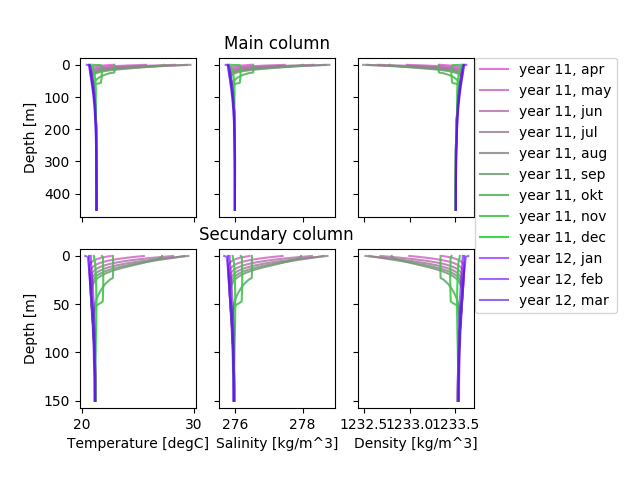
\includegraphics[width=0.9\textwidth,keepaspectratio]{Conv_only.png}
\caption{A typical year of a run with mixing. This data was generated using an instability check in the top node instead of a whole column check for instability.}
\label{fig:Conv_Only}
\end{figure*}

% % Fig with summer mixing, kleine uitslag
% %-------------------
\begin{figure*}
%% subfig 1
\begin{subfigure}[h]{0.7\textwidth}
\centering
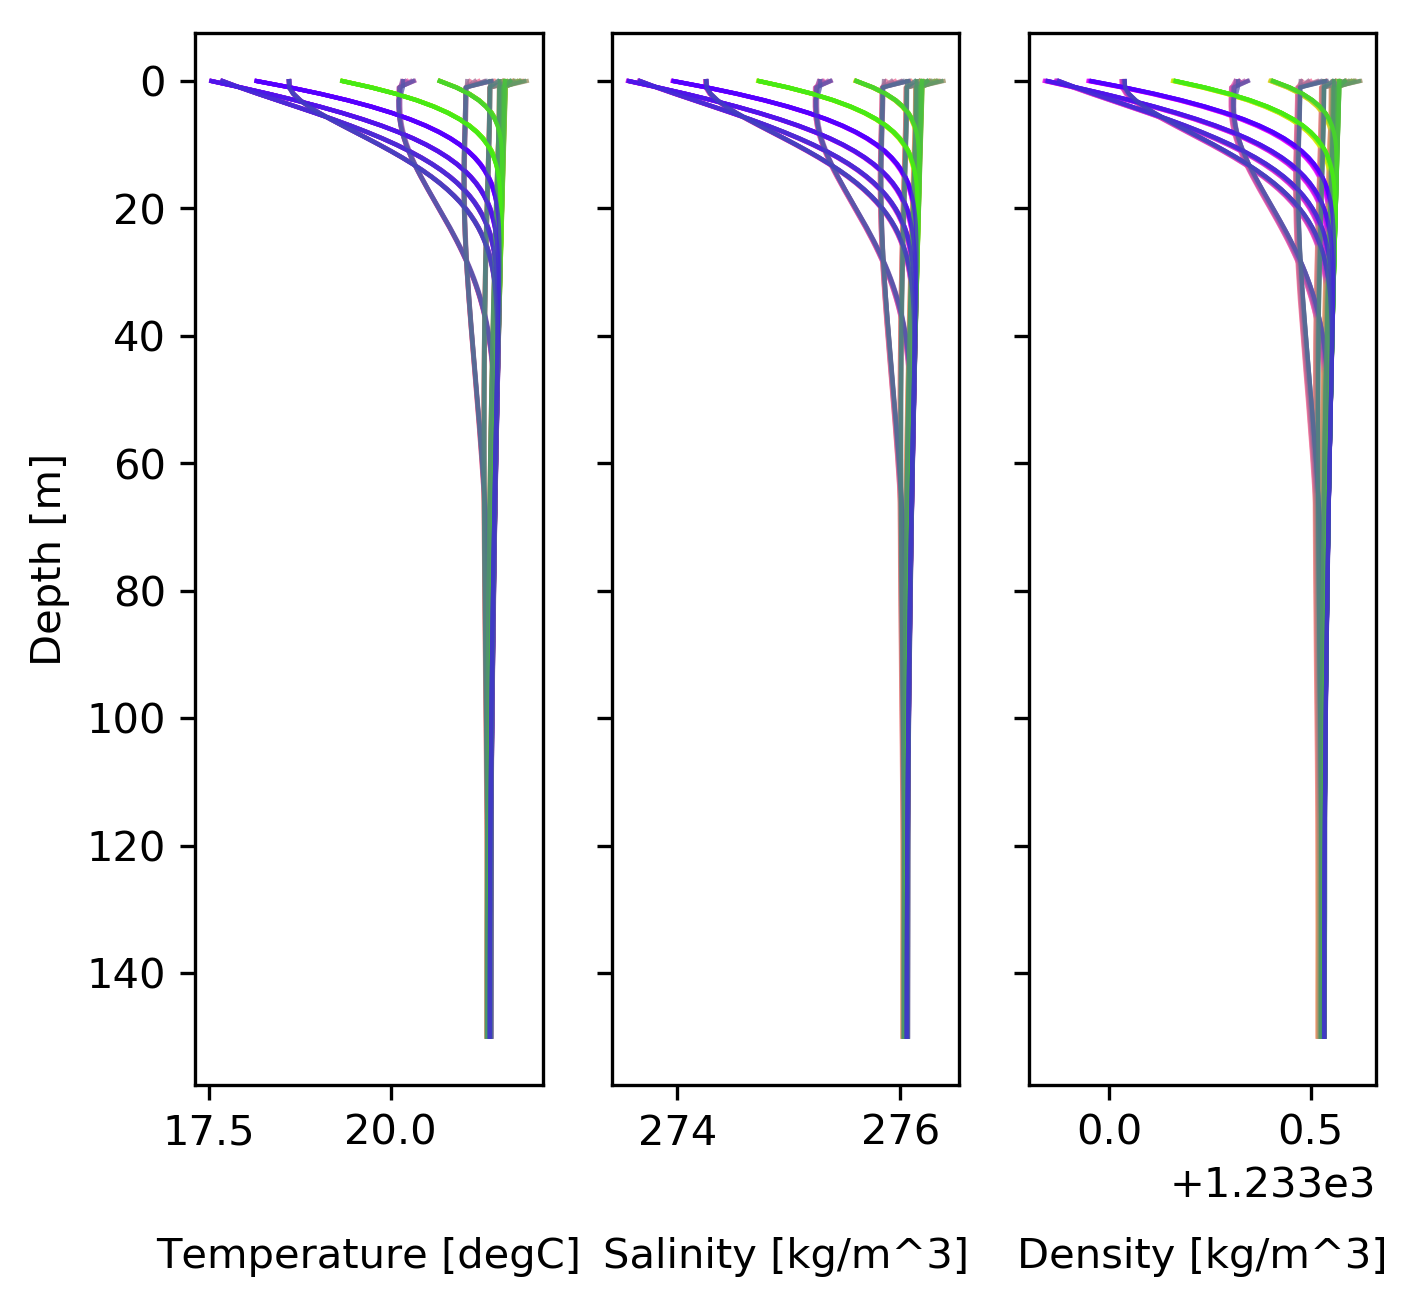
\includegraphics[width=\textwidth,keepaspectratio]{summer_mixing.png}
\end{subfigure}\hfill
%% subfig 2
\begin{subfigure}[h]{0.20\textwidth}
\centering
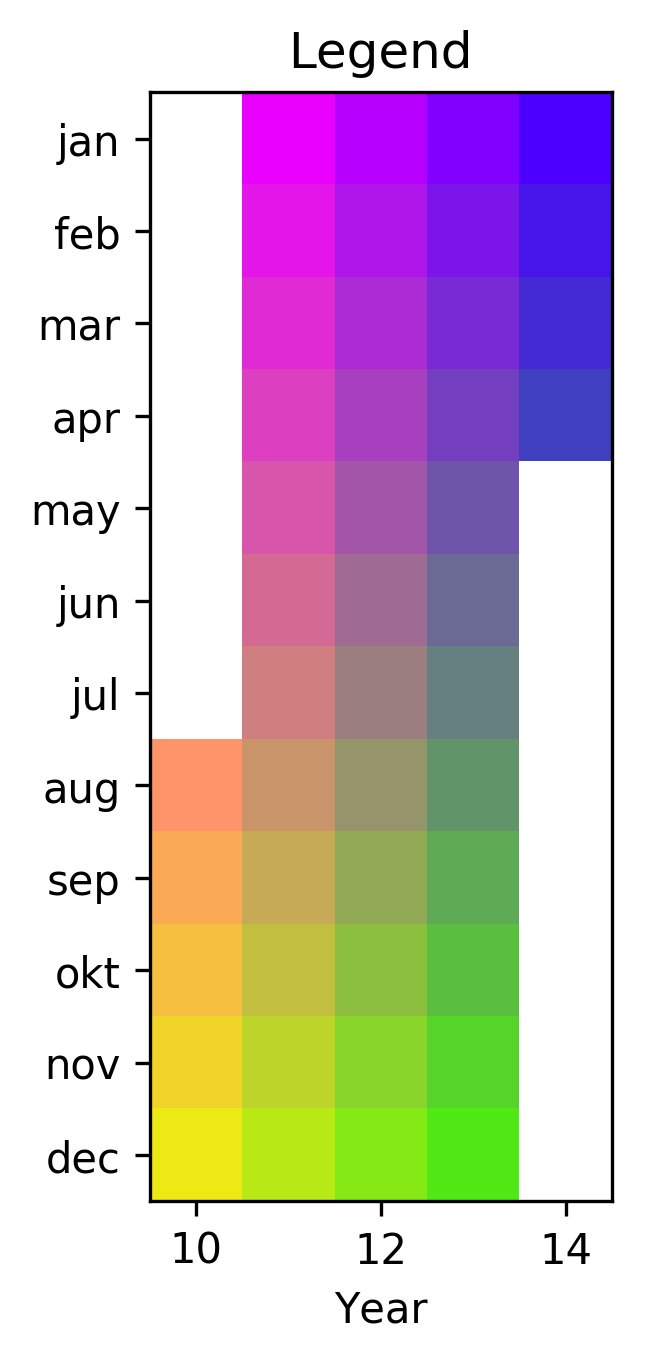
\includegraphics[width=1.0\textwidth,keepaspectratio]{summer_mixing_Legend.png}
\end{subfigure}\hfill
\caption{Model run with mixing. The evaporation amplitude was doubled, inducing mixing in summer.}
\label{fig:summer_mixing}
\end{figure*}

\subsubsection{Discussion}
Concerning the transition, as shown in figure~\ref{fig:Transition}, the mixing should start in April. This is namely the moment from where mixing is allowed, and the density in the top node is higher then the rest of the column. The mixing does however not occur until October, as read from figure~\ref{fig:Transition}. The cause of this is that the code begins the instability check by checking whether the top node is more dense then the one below it. Since, in April, year 10, the top node is as dense as the one below it, is considered stable. Even if the top twenty metres are more dense then the water below it. This situation generally only occurs during the transition, for the top nodes are always the first to move, meaning that any instability will be initialized there first. The exception to this is a source-sink pulse, pulling salt from the bottom of the marginal basin, without directly affecting the water in the middle of the column. In order to have mixing in the bottom of the column to resupply salt to the bottom of the marginal basin and restore the density instability, a more rigorous check for instability is required, mentioned in section \ref{sect:stability_methods}. When checking the column for instability both from the top node down and from the bottom node up, the salt deprivation in the bottom of the marginal basin after flow is solved in this way. The artifact that arises during the transition period as shown in figure~\ref{fig:Transition} does however remain.
The alternative method is to check each individual node for stability. This method solves both the artifact during the transition and the salt deprivation in the bottom of the marginal basin. In practice, the whole column check can take up to an order of magnitude longer to run. This is not only due to the increase in effort to check for the whole column, but mainly due to the limiting factors shown in equation~\ref{eq:FCTS_limits}, where the highest diffusivity in the column determines the size of the time step. A few scattered unstable nodes can therefore significantly impact the run time. 

It turns out however, that the whole column check is more stable then the top-down, bottom-up check. This is elaborated upon in section \ref{sect:totals_problem}.

\subsection{Summer mixing}
The stability of the column is mainly determined by the density of the surface waters and therefore, ultimately determined by the balance between $\alpha T$ and $\beta S$ (equation \ref{eq:state}) at the surface. By altering either the heat flux or the evaporation, the stability behavior of the column can be investigated.

\subsubsection{Results}
Figure \ref{fig:summer_mixing} shows the results of a run with an evaporation amplitude of 0.6 rather then the standard 0.3. The mixing now occurs in summer while the column is stable in winter. The overall shape of the profile is rather the same, but the density is now almost a direct copy of the temperature and salinity rather than a mirror image, as is the case in figure \ref{fig:Conv_Only}. 


\subsubsection{Discussion}
\label{sect:Summer_mixing_discussion}
When $\alpha T$ is dominant over $\beta S$, as is the case in figure \ref{fig:Conv_Only}, the column mixes in winter, for the density is inversely dependent on
the temperature. In figure \ref{fig:summer_mixing} however, $\beta S$ is dominant over $\alpha T$. The subsequent extra saline surface waters in summer, result in an unstable column, despite its high temperature. In winter the opposite is true, where the surface waters are fresh enough to remain stable despite the low temperatures.

The periods of mixing in the dead sea are determined by the temperature profile. For lack of knowledge on the periods of mixing during the MSC, the assumption is made here that this was also the case for the MSC. Keep in mind that the foundation for this assumption is not very solid. Periods of low river discharge into the Mediterranean could even have resulted in almost year-round mixing with high salinity creating instability in summer and low temperatures creating instability in winter. 


\subsection{Source sink and advection}
% Fig SS
%-------------------
\begin{figure*}
%% subfig 1
\begin{subfigure}[h]{0.7\textwidth}
\centering
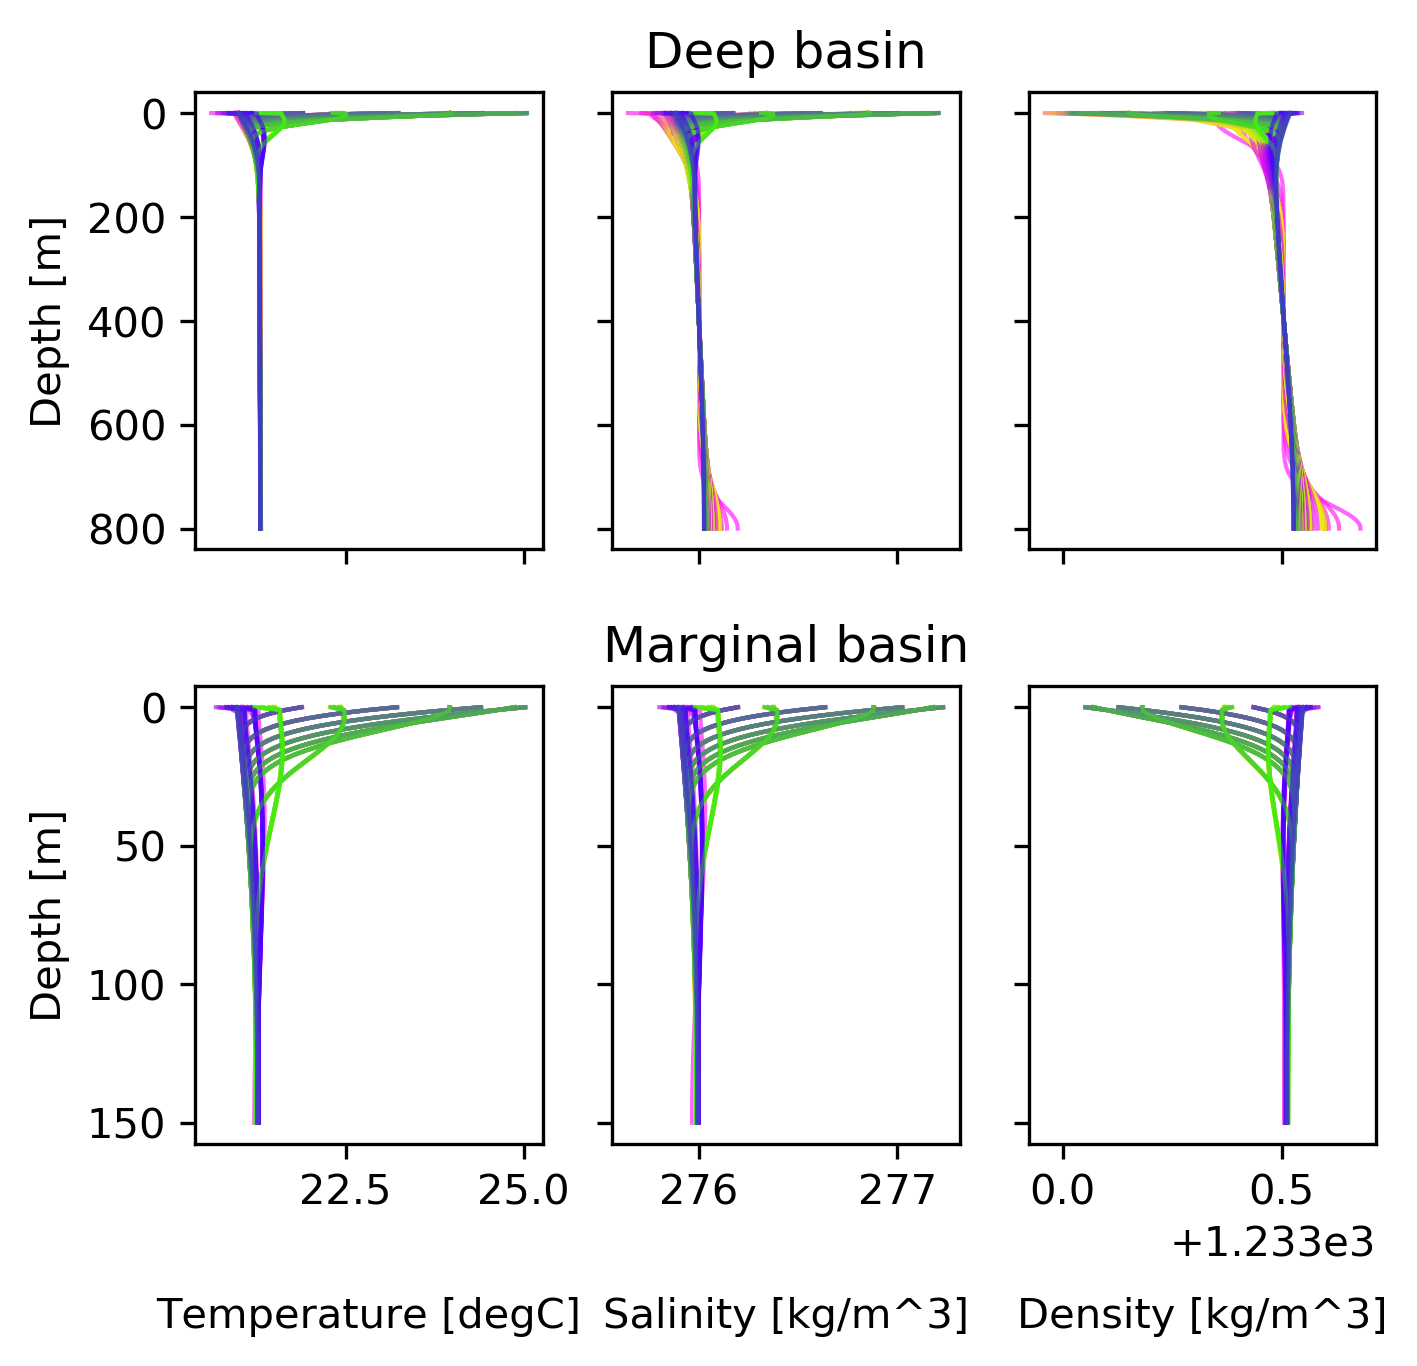
\includegraphics[width=\textwidth,keepaspectratio]{SS_no_adv.png}
\end{subfigure}\hfill
%% subfig 2
\begin{subfigure}[h]{0.23\textwidth}
\centering
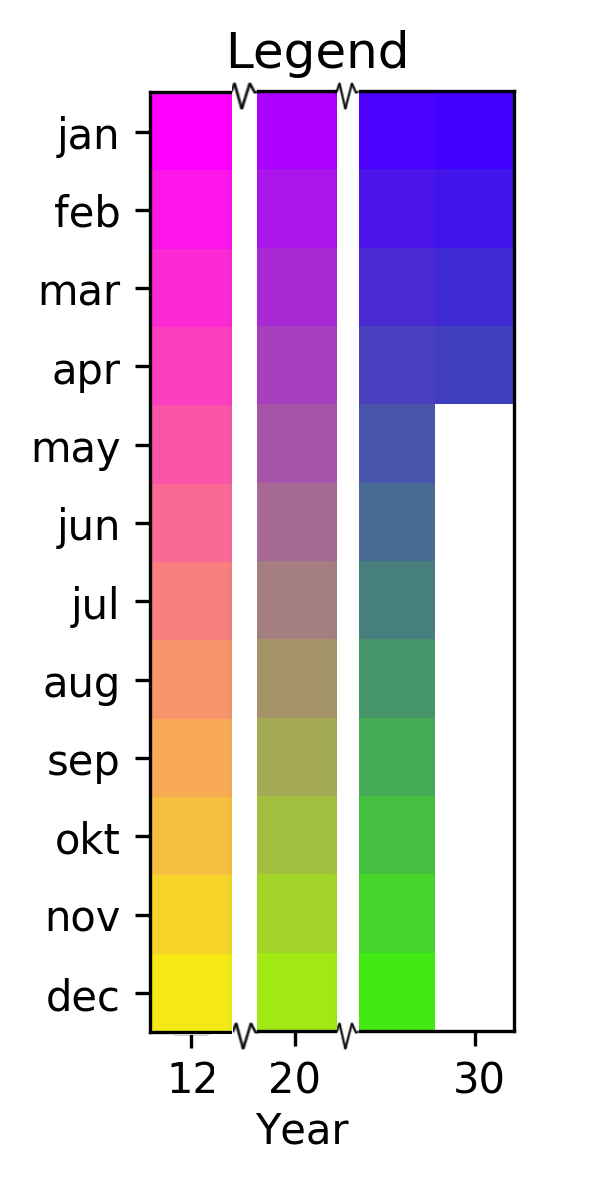
\includegraphics[width=\textwidth,keepaspectratio]{12-30_reduced_legend.png}
\end{subfigure}\hfill
\caption{Standard model case with source-sink and no advection. The situation shown is right after flow between the two basins occurred.}
\label{fig:no_adv}
\end{figure*}




\begin{figure*}
%% subfig 1
\begin{subfigure}[h]{0.7\textwidth}
\centering
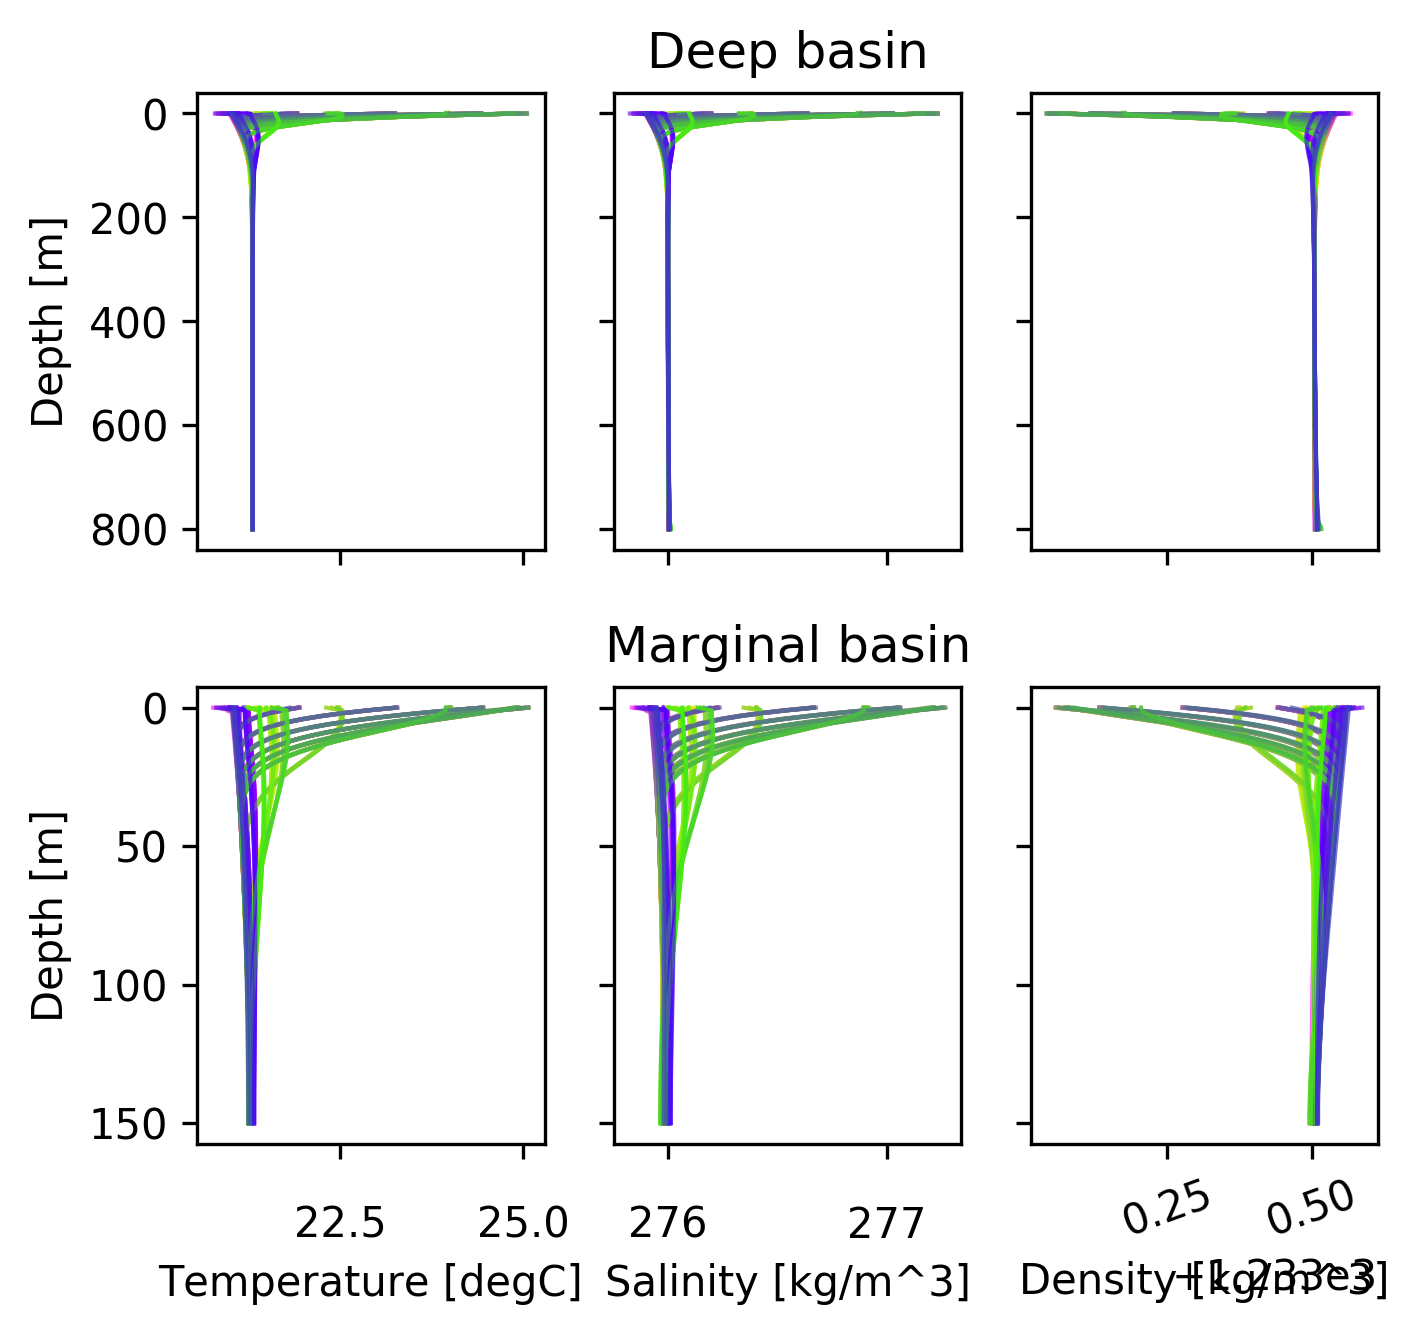
\includegraphics[width=\textwidth,keepaspectratio]{with_adv_150m.png}
\end{subfigure}\hfill
%% subfig 2
\begin{subfigure}[h]{0.20\textwidth}
\centering
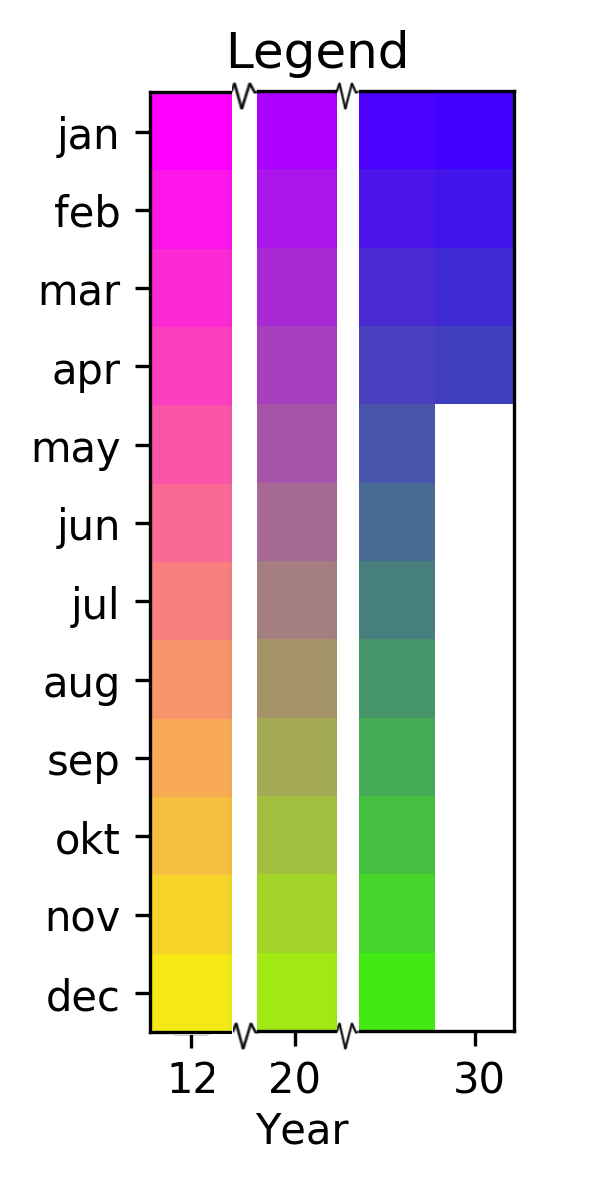
\includegraphics[width=\textwidth,keepaspectratio]{12-30_reduced_legend.png}
\label{fig:}
\end{subfigure}\hfill
\caption{Standard model case with advection.}
\label{fig:with_adv_geen_uitslag}
\end{figure*}



\subsubsection{Results}
% Wrap-Fig Legend for discuss adv and Fig SS
%----------------------------------------
A result of a standard model case (appendix \ref{app:standard_parameters}) with no advection and an increased exchanging flow from 1e-5 to 5e-3 Sv is shown in figure \ref{fig:no_adv}. The result of the same case but \textit{with} advection is shown in figure \ref{fig:with_adv_geen_uitslag}. In both instances, part of the column mixes during fall and the entire column mixes from January to March, in both the deep and marginal basins. The marginal basin of figure \ref{fig:no_adv} very strongly resembles figure \ref{fig:Conv_Only}, as does the deep basin with the exception of the increased salinity at its bottom. Only one pulse of exchanging flow occurred. This pulse was large enough to create a clear salinity access at the bottom of the deep basin in one exchange.
In a case with advection, the dense water body at the bottom of the deep basin is generally a lot less pronounced or not present at all, as is the case in figure \ref{fig:with_adv_geen_uitslag}. A model run with advection and a flow of 40 Sv is shown in figure \ref{fig:with_adv_large_effect}. With this large exchanging flow, the workings of the code can be easily analyzed in report format, for the effects are large enough to visualize in a plot.% This figure is discussed in section \ref{sect:large_effect}. 


% % Fig with adv, ook uitslag onderaan
% %-------------------
% \begin{figure*} 
% \centering
% \includegraphics[width=1\textwidth,keepaspectratio]{"with adv good".png}
% \caption{Model run with advection. A color legend is shown in figure \ref{fig:legend}.}
% \label{fig:with_adv}
% \end{figure*} \todo{mention why basin is so shallow}


% % Fig with adv, grote uitslag, genummerd
% %-------------------
\begin{figure*}
%% subfig 1
\begin{subfigure}[h]{0.7\textwidth}
\centering
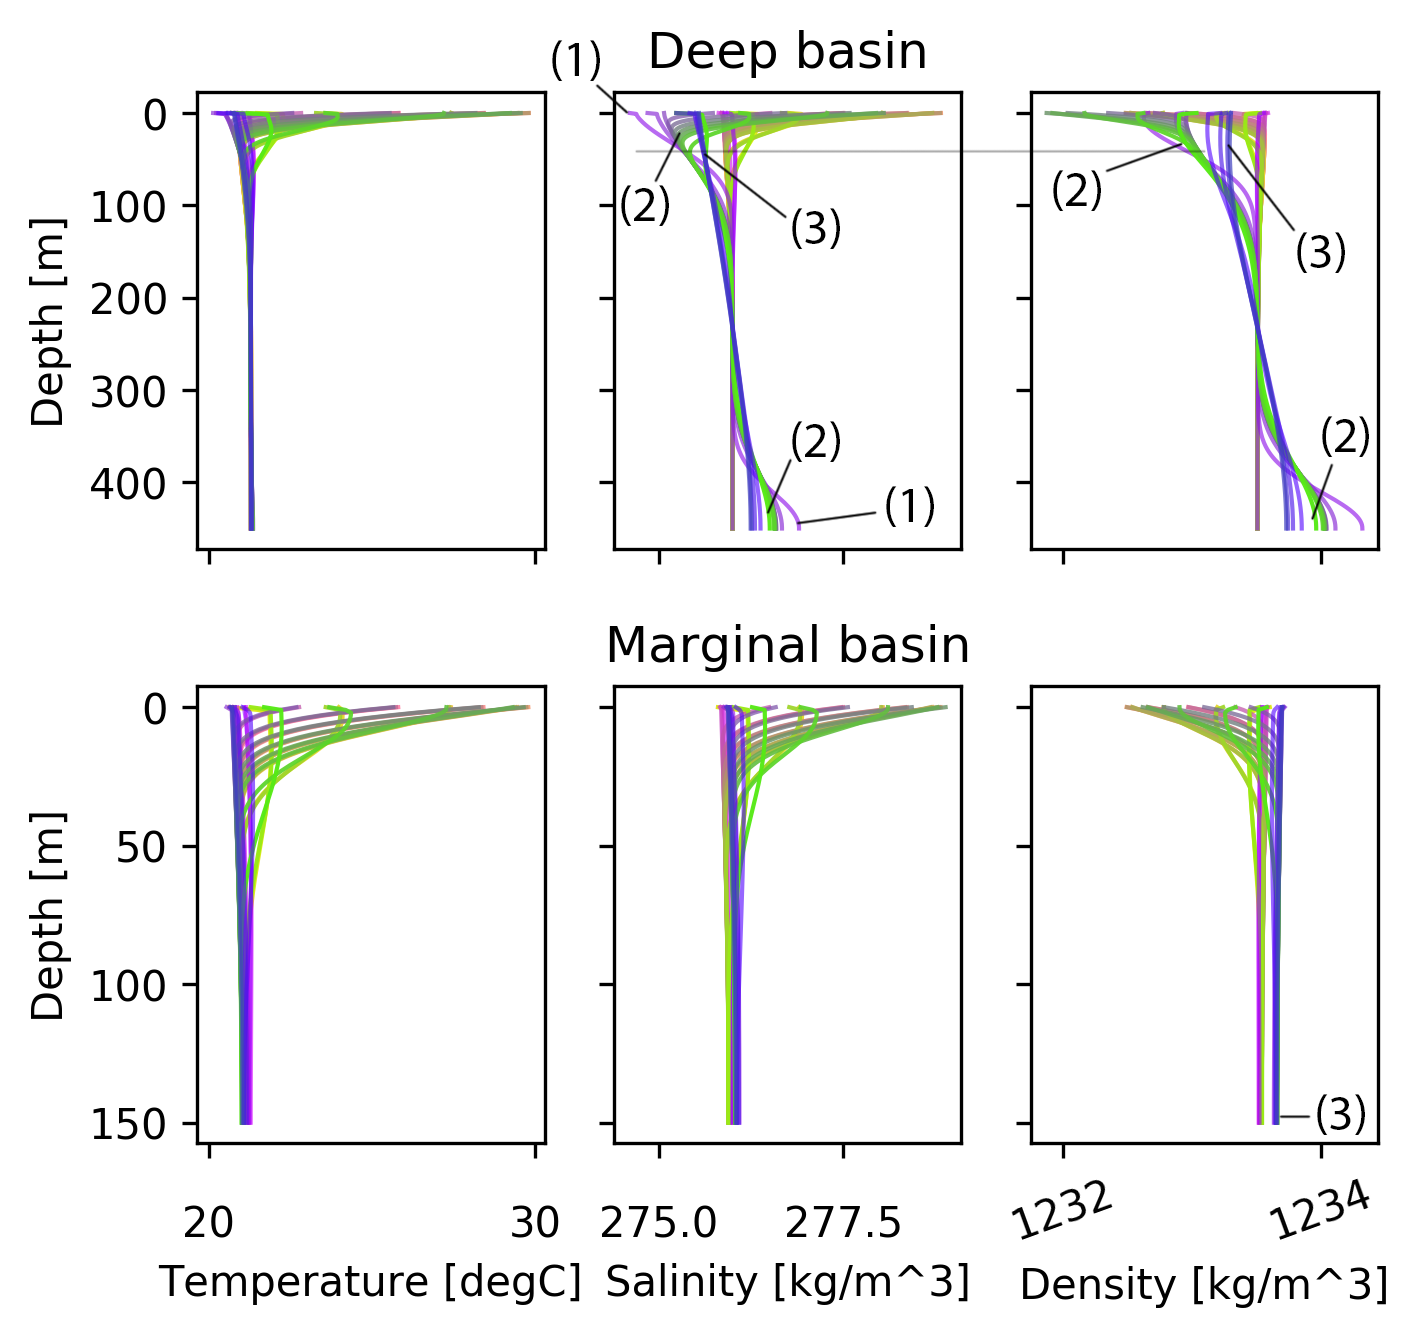
\includegraphics[width=\textwidth,keepaspectratio]{with_adv_large_effect_40SV_altered.png}
\end{subfigure}\hfill
%% subfig 2
\begin{subfigure}[h]{0.20\textwidth}
\centering
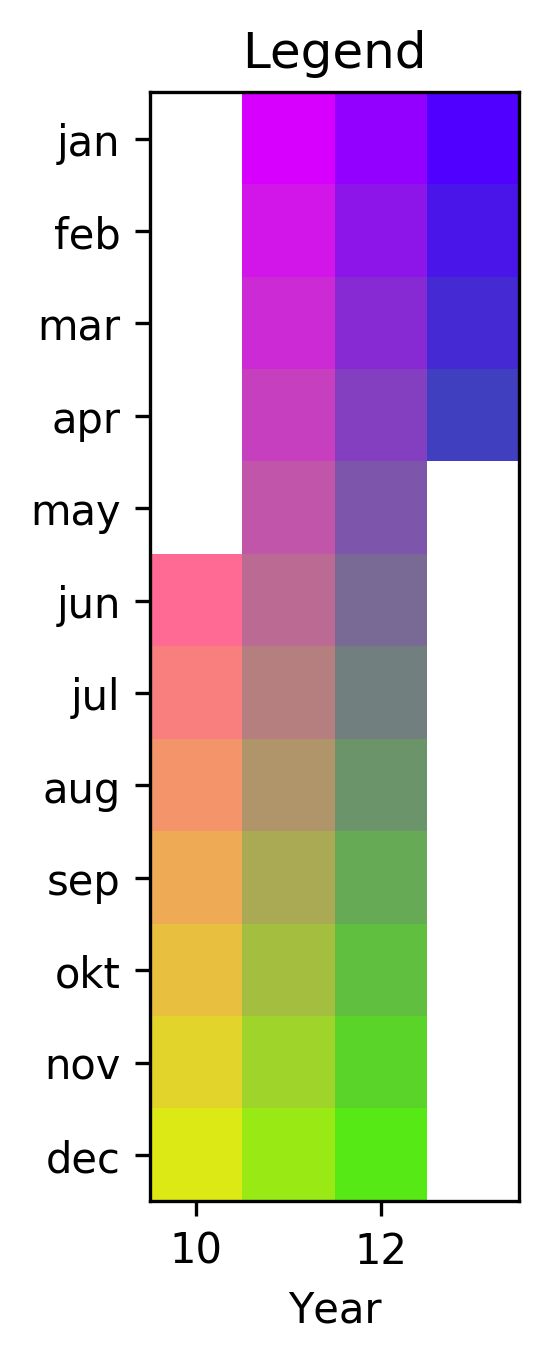
\includegraphics[width=1.0\textwidth,keepaspectratio]{with_adv_large_effect_40SV_Legend.png}
\end{subfigure}\hfill
\caption{Standard model case with advection and an exchanging flow of 40 Sv. (1): initiation of the exchanging flow (2): slow decrease of anomaly (3): mixing. }
\label{fig:with_adv_large_effect}
\end{figure*}

\subsubsection{Discussion}
\label{sect:SS_and_adv_discussion}
% The exchange between the marginal basin and the deep basin, shown in figure \ref{fig:no_adv}, lowers the total amount of salt in the marginal basin, for the water that flowed out is more saline then the water that flowed in. Then, when mixing occurs during each consecutive summer in the marginal basin, saline water is resupplied to the bottom waters. In the deep basin, the saline water body is stable but is shrinking due to diffusion. As the deep saline water is largely diffused away, a new dense plume from the marginal basin may arrive to repeat the process. 
An initial pulse of exchanging flow occurres because the bottom of the marginal basin experiences slight changes in temperature and salinity whereas the bottom of the deep basin is too deep to experience changes created through surface forcing. The exchange between the marginal basin and the deep basin, shown in figure \ref{fig:no_adv}, slightly lowered the total amount of salt in the marginal basin, for the water that flowed out was more saline then the water that flowed in. While salt is directly resupplied to the bottom of the marginal basin due to the unstable density configuration, the excess salt in the bottom of the deep basin created a stable configuration. This excess salinity only decreases due to the background diffusion. When the excess salinity has been reduced to its original state due to the background diffusion, and the bottom of the marginal basin is sufficiently replenished, a new pulse could occur. However, since the first pulse slightly altered the average salinity of both basins, it can take years for the marginal basin bottom waters to once again become more saline then the bottom waters of the deep basin. In fact, if the difference in average salinity is larger then the yearly difference due to forcing, no second pulse will ever occur, for no other factors influence the density distribution in this model scenario. Realistically, this scenario is impossible for it would create space problems due to an incomplete flow cycle caused by the lack of advection.
The scenario shown in figure \ref{fig:with_adv_geen_uitslag} was initialized with the same conditions as the one shown in figure \ref{fig:no_adv} except that, during the periods of exchange, advection was allowed. As is evident when comparing the two figures, advection completely removed the effect of the source-sink term. Any water that arrived in the deep basin was directly being advected up, thus not allowing for a dense water body at the bottom of the deep basin to form. In order to investigate how the model handles these advection situations, the model was run with a flow of 40 Sv. This amount of volume is in no way realistic but makes it easier to investigate the workings of the model. Figure \ref{fig:with_adv_large_effect} shows an annotated plot of this model run. This figure shows that right after the initiation of flow (1), the deep basin is fully stable with denser than average waters at the bottom and the least dense water at the top. Most of any negative density anomaly at the base of the marginal basin is directly resupplied by mixing. From the initiation of flow (1) until the next mixing during winter (3), the salt anomalies dissipate slowly due to diffusion (2). When the columns mix in winter, the bottom waters of the deep column are unaffected due to their stable state. During this mixing period, some salt is resupplied to the bottom of the basin, leading to a small jump in the density plot. 
Aside form the large amount of flow required for this effect to be visible, an issue becomes apparent when analyzing the results. Due to the technical choice of imitating the flow with the source-sink term, combined with this large flow of 40 Sv, the bottom waters of the deep basin become significantly more saline then the bottom of the marginal basin ever was. 

In order to obtain a dense saline brine at the bottom of the deep basin, the bottom of the marginal basin clearly needs to be significantly more saline then is achieved through the parameters used in the runs shown so far. This could be done by increasing the total amount of salt in the marginal basin through net evaporation or by allowing for faster transport of salt to the bottom of the marginal basin. The latter can be achieved by decreasing the basin depth or increasing the amount of diffusion during mixing. A combination of these is likely required to achieve the sought effect. These factors will be discussed in section \ref{sect:imprtant_parameters}.

% \subsection{Examining an extreme example with all features activated}
% \label{sect:large_effect}
% \subsubsection{Results}
% A way to obtain a salt water body at the bottom of the deep basin is to have an extreme amount of flow between the basins when the density trigger is satisfied. In figure \ref{fig:with_adv_large_effect}, this flow was forty Sv, which is over forty times the present day flow through the Strain of Gibraltar. This amount of water movement is clearly unrealistic but it does allow us to examine the workings of the model. 
% When the density trigger is activated and flow is initiated in the winter of year 12 ( indicated as (1) in figure \ref{fig:with_adv_large_effect}), salt is clearly extracted form the top of the deep basin and added to the bottom. The advection already moved a lot of salt up in the main basin already, which is why, despite the large amount of flow, the offset is not nearly as large as in figure \ref{fig:no_adv}. This is also visible in the relatively low gradient of the January year 12 curve, indicated with (1) in figure \ref{fig:with_adv_large_effect} when compared to the initial after-flow profile of figure \ref{fig:no_adv}. In the marginal basin, the opposite has happened but this is not visible in the figure. Any low-density anomaly at the bottom of the marginal basin is unstable and is therefore resupplied with salt via mixing until it has a similar salinity to the water above it. Note that this mixing does not involve the whole of the marginal basin but only the unstable bottom. While instabilities in the marginal basin are covered up through mixing, the entire deep basin now has a stable density configuration. Since at this point there is no mixing in the deep basin, the anomalies created by the flow are slowly decreasing in size because of the background diffusivity (2). In the winter of year 13 ( indicated with (3) ), the anomaly at the top of the main basin is straightened out more rapidly. In the marginal basin, mixing in this period brings salt to the bottom of the basin, seen in the density plot as a small offset.
% 
% \subsubsection{Discussion}

\FloatBarrier
% %%%%%%%%%Standard run
% \begin{figure*}
% %% subfig 1
% \begin{subfigure}[h]{0.7\textwidth}
% \centering
% 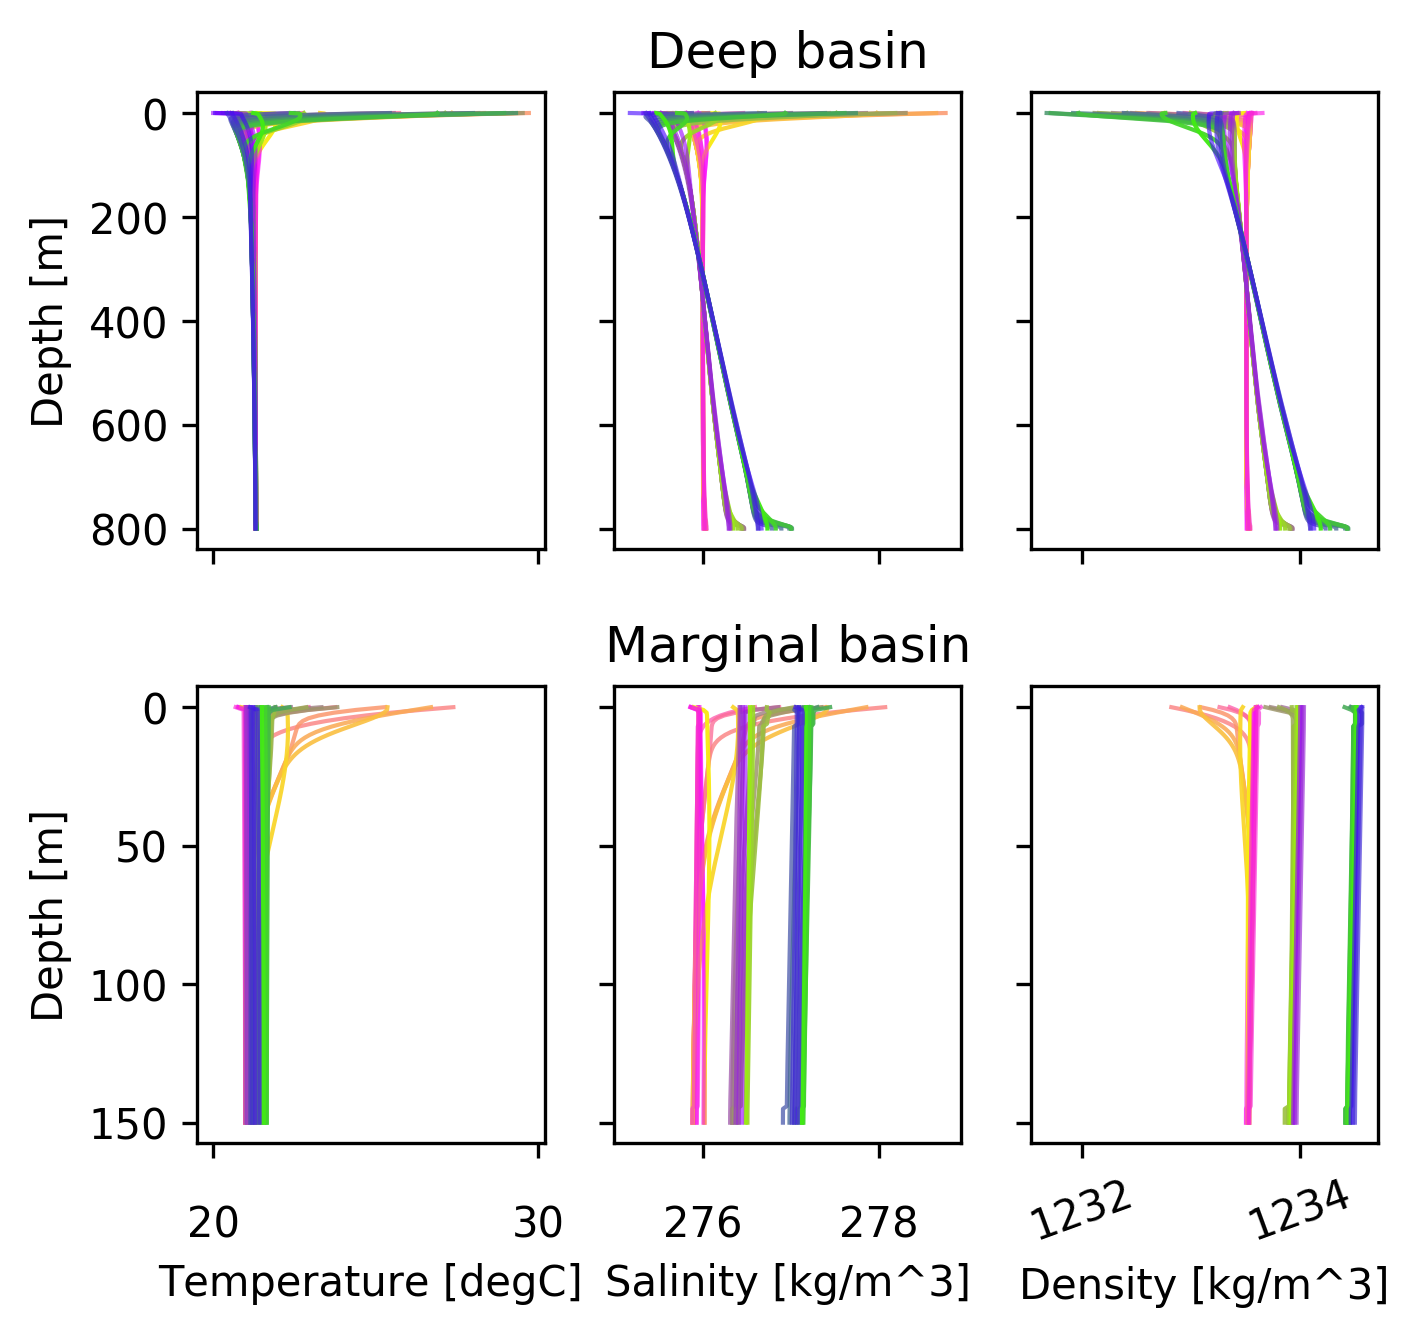
\includegraphics[width=\textwidth,keepaspectratio]{standard_run.png}
% \end{subfigure}\hfill
% %% subfig 2
% \begin{subfigure}[h]{0.20\textwidth}
% \centering
% 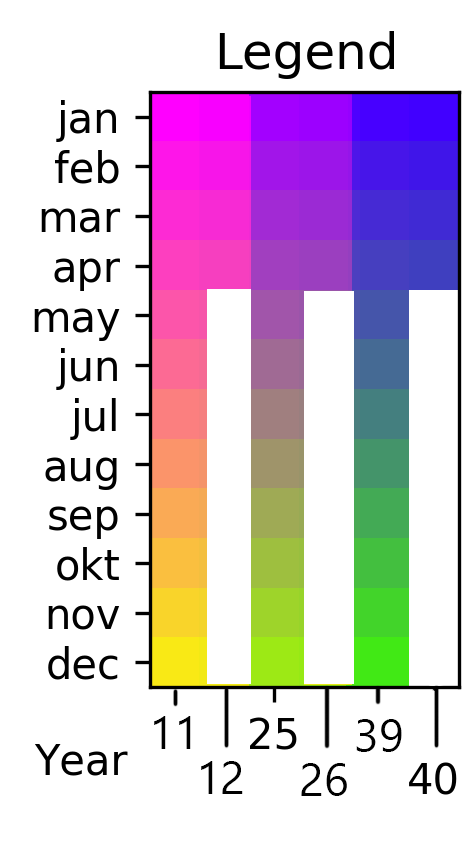
\includegraphics[width=\textwidth,keepaspectratio]{40yr_reduced_Legend.png}
% \label{fig:}
% \end{subfigure}\hfill
% \caption{Model run with advection. The same input parameters as the run shown in figure \ref{fig:no_adv} were used.}
% \label{fig:with_adv_geen_uitslag}
% \end{figure*}


%%%%%%%%%%%%%%%%%%%%%%%%%%%%%%%%%%%%%%%%%%%%%%
%%%%%%%%%%%%%%%% Main section %%%%%%%%%%%%%%%%
%%%%%%%%%%%%%%%%%%%%%%%%%%%%%%%%%%%%%%%%%%%%%%

\section{Important factors on the formation of a deep brine}
\label{sect:imprtant_parameters}
As discussed in the previous section, the most relevant parameters are those that greatly influence the amount of salt in the bottom of the marginal basin. Likely candidates are the marginal basin depth, the background diffusion and net evaporation. In order for a saline marginal basin to have a significant impact on the salinity of the deep waters, the flow between the basins would need to be sufficient but should not reach unrealistic proportions, as is the case in figure \ref{fig:with_adv_large_effect}. When the exchanging flow is small, the comparative volumes of the basins needs to be such that the total amount of salt in the marginal basin is not negligible when compared to that of the deep basin. These factors and their impact on the possible existence of a deep salt brine will therefore be investigated in the following sections.

% %% 300m stable
% \begin{figure*}
% %% subfig 1
% \begin{subfigure}[h]{0.7\textwidth}
% \centering
% 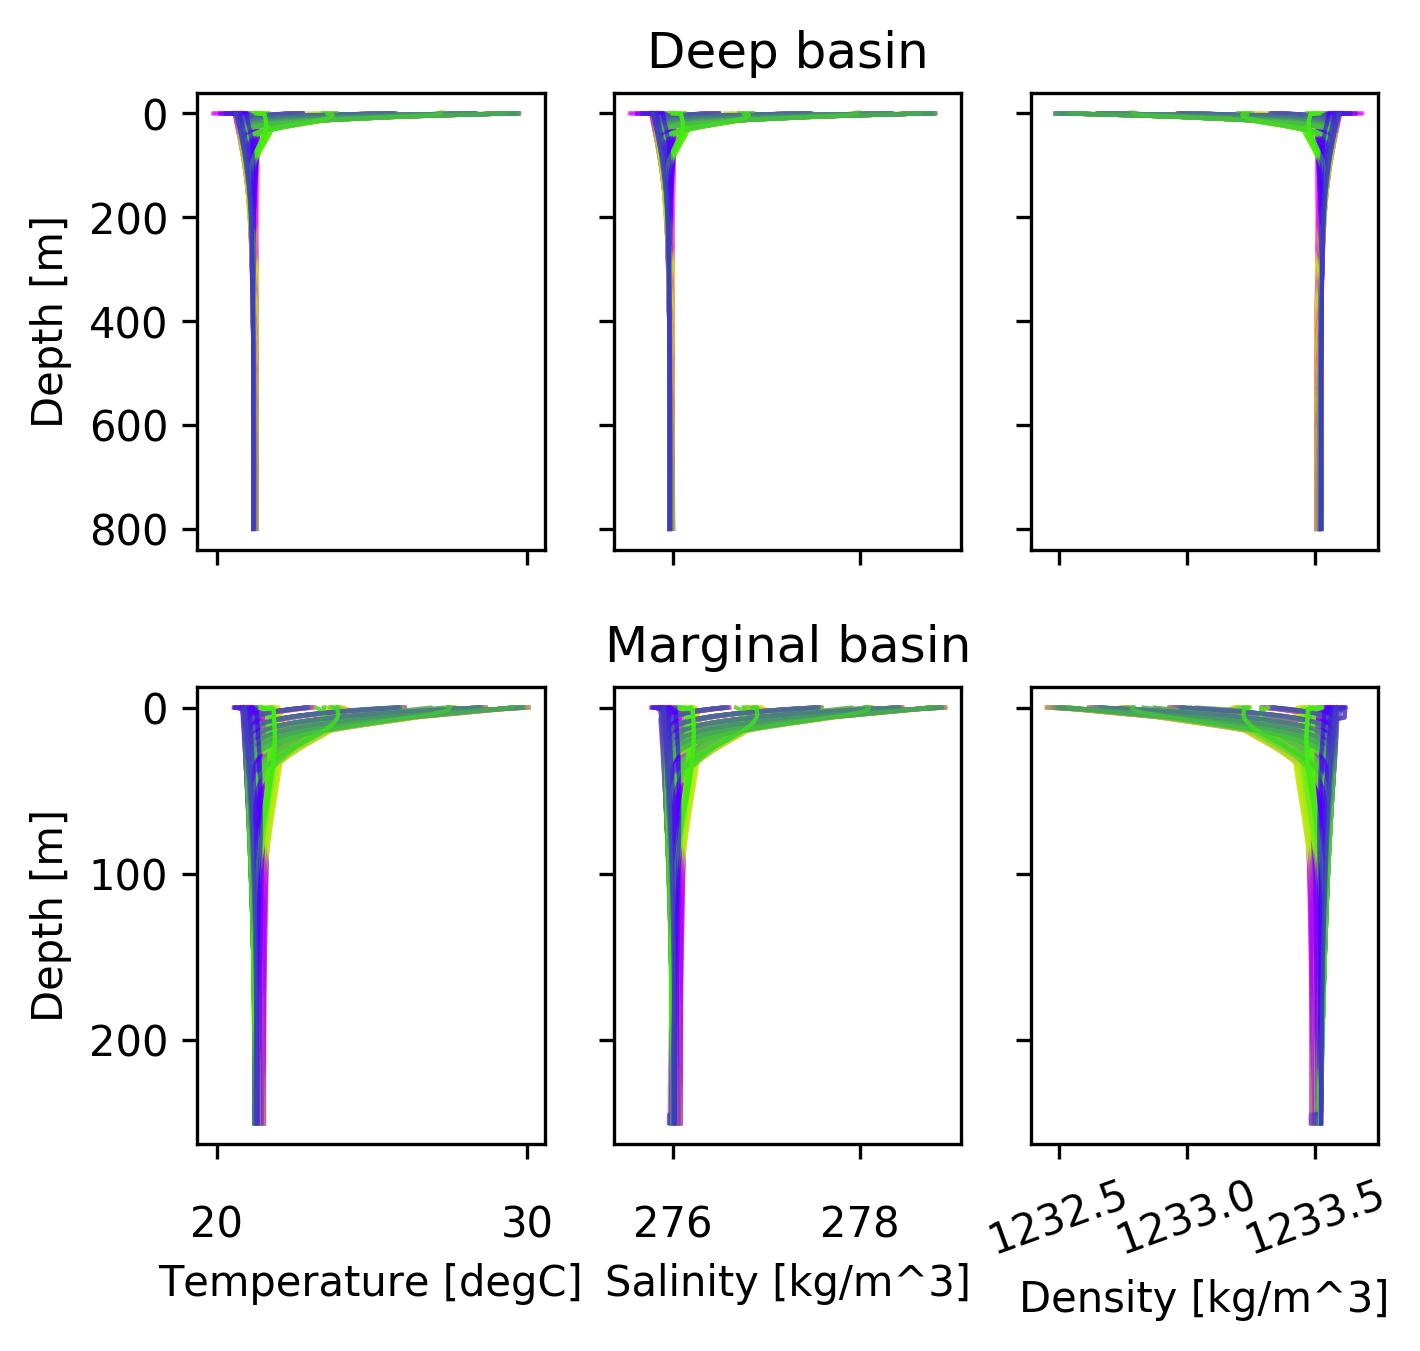
\includegraphics[width=\textwidth,keepaspectratio]{with_adv_stable.png}
% \end{subfigure}\hfill
% %% subfig 2
% \begin{subfigure}[h]{0.20\textwidth}
% \centering
% 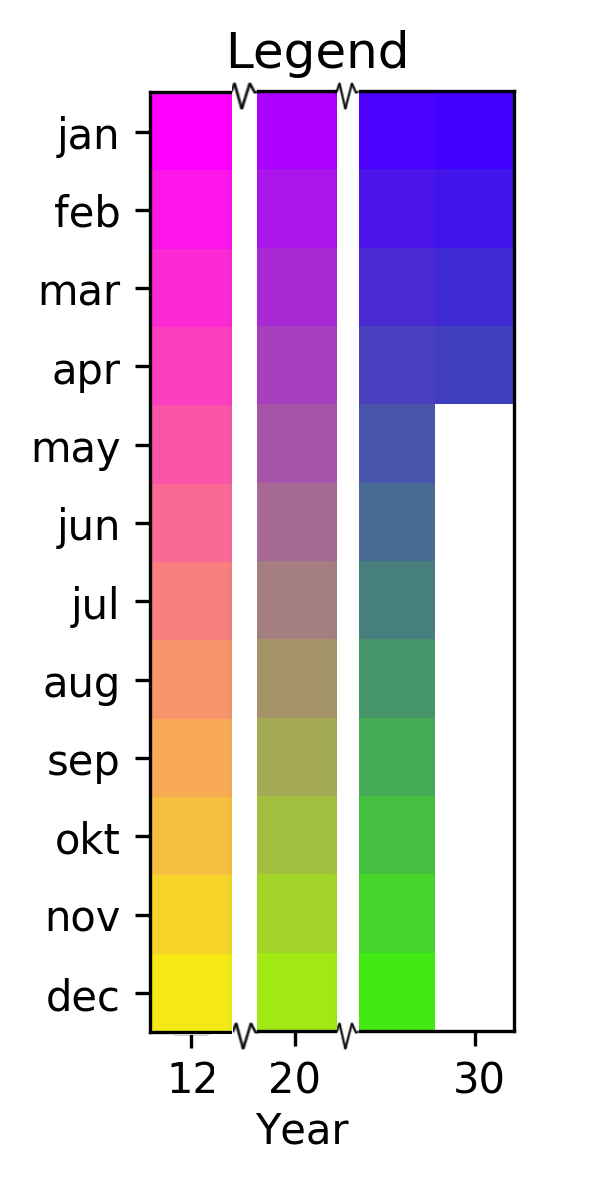
\includegraphics[width=\textwidth,keepaspectratio]{12-30_reduced_legend.png}
% \label{fig:}
% \end{subfigure}\hfill
% \caption{Standard model run with increased depth of the marginal basin. }
% \label{fig:with_adv_geen_uitslag}
% \end{figure*}

%% Shallow mar basin fig 60m
\begin{figure*}
%% subfig 1
\centering
\begin{subfigure}[h]{0.70\textwidth}
\centering
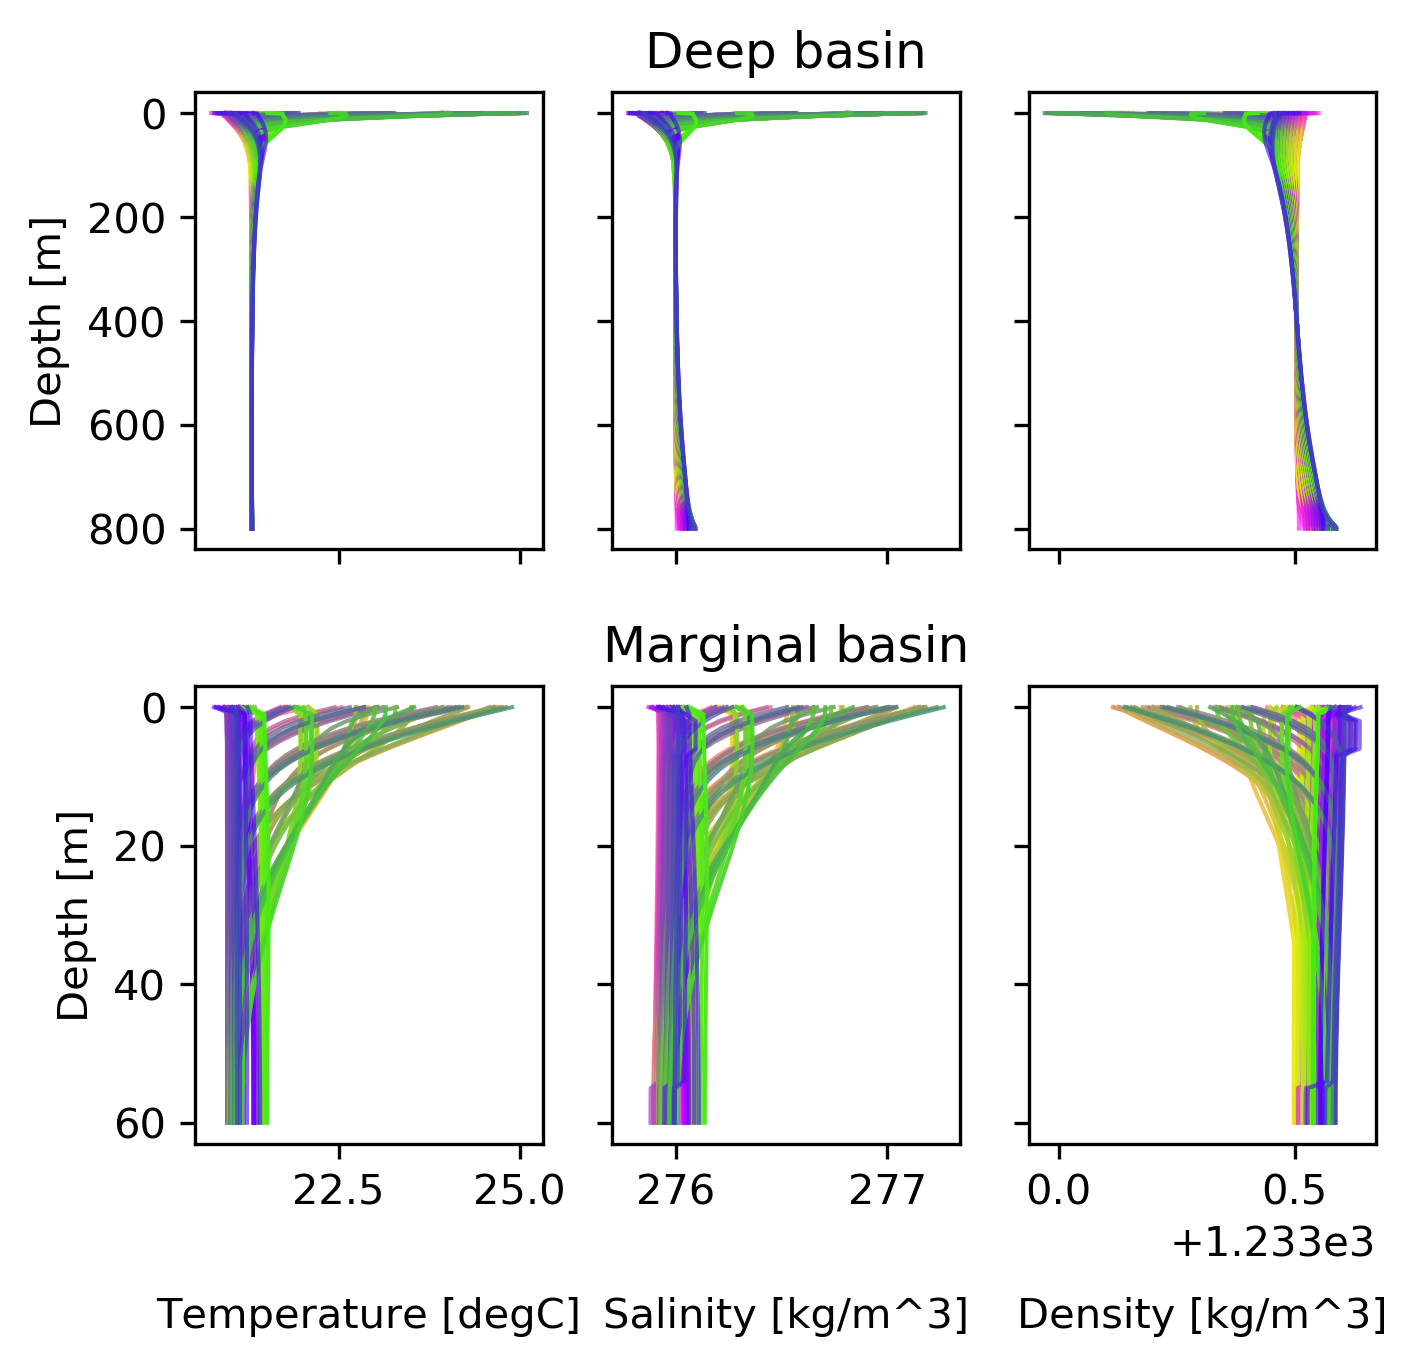
\includegraphics[width=\linewidth,keepaspectratio]{60m_mar_depth_40yr.png}
\end{subfigure}\hfill
%% subfig 2
\begin{subfigure}[h]{0.20\textwidth}
\centering
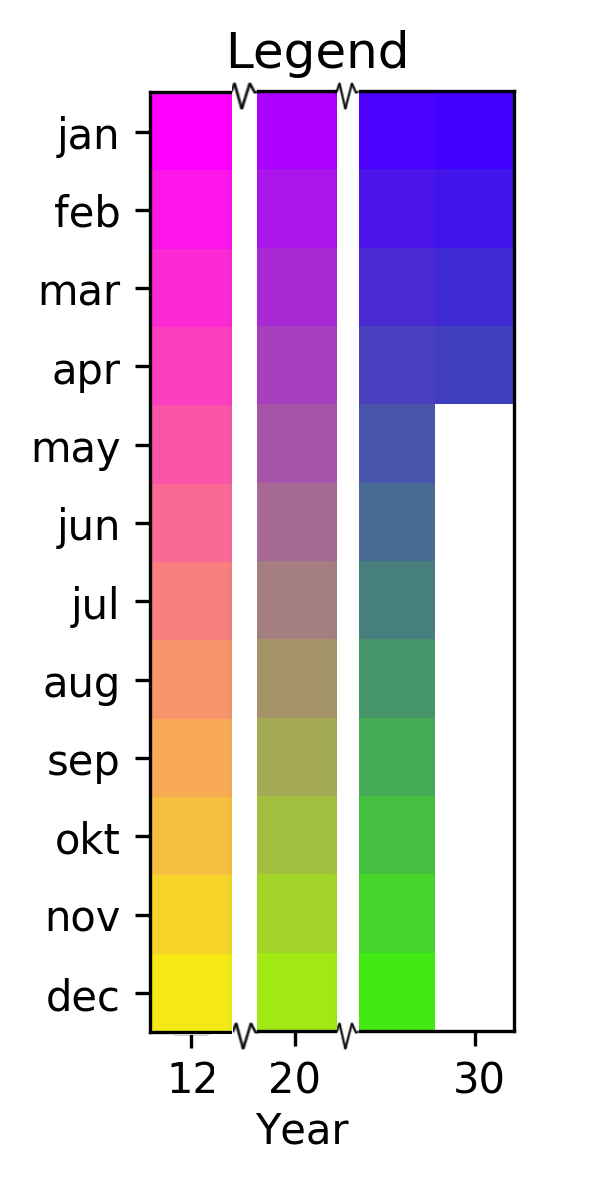
\includegraphics[width=\linewidth,keepaspectratio]{12-30_reduced_legend.png}
\end{subfigure}\hfill
\caption{Standard model case with a very shallow marginal basin. Three periods, those at 11,25 and 39 years, are shown.}
\label{fig:Very_shallow_basin}
\end{figure*}

% %% Shallow mar basin fig 60m MEAN VALUES
% \begin{figure*}
% \centering
% 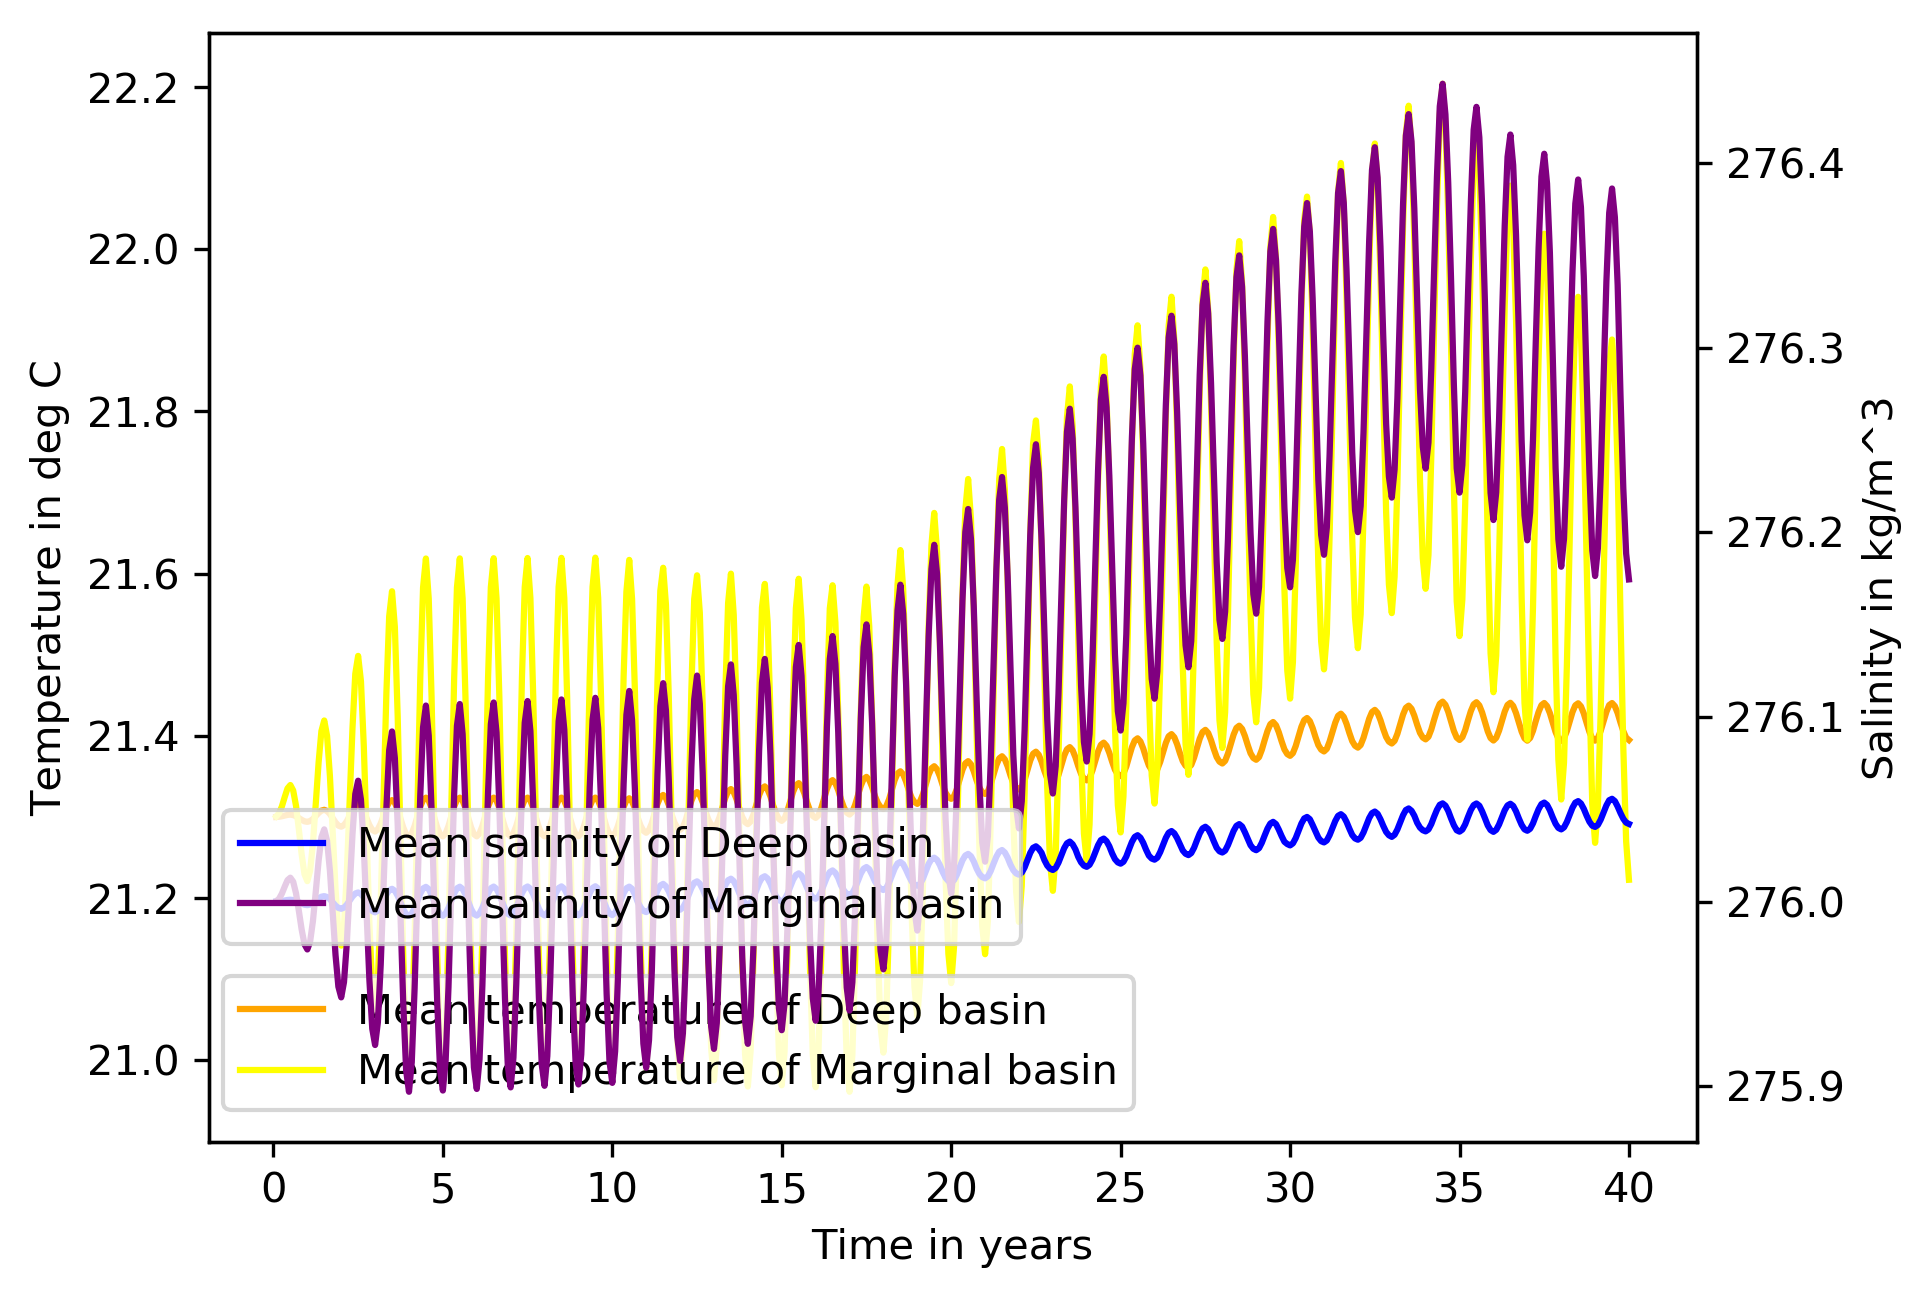
\includegraphics[width=\textwidth,keepaspectratio]{60m_mar_depth_40yr_totals.png}
% \caption{Mean values over time corresponding to the scenario shown in figure \ref{fig:Very_shallow_basin}}
% \label{fig:Very_shallow_basin_means}
% \end{figure*}\hfill

% % Fig with high background diff
% %-------------------


\subsection{Results}

\subsubsection{Marginal basin depth}
\label{sect:mar_basin_depth}
Figure \ref{fig:Very_shallow_basin} shows the results of a standard case with a 60m deep marginal basin. A minor increase in salinity has been achieved. Incremental steps are made towards the redistribution of salinity, rather then the one pulse in case \ref{fig:no_adv}. 


\subsubsection{Background diffusivity}
Figure \ref{fig:high_db_success} shows the results of a standard run and a background diffusivity of 1e-3.0. The depth to which the surface forces penetrate, as well as the maximum deviation from the average temperature at the surface differ from the previous scenario. The bottom of the marginal basin experiences significance variation throughout the year. A very small increase in salinity is observed in the bottom of the deep basin, of which the largest pulse occurred in the first year after the spinup. The average values of both basins were almost unaffected by the exchanging flows as can be observed in figure \ref{fig:high_bg_diff_means}.

\subsubsection{A depth and diffusivity hybrid}
A decrease in marginal basin depth on top of an increased background diffusivity (figure \ref{fig:hybrid}) had a large effect on the salinity at the bottom of the deep basin compared to the case shown in figure \ref{fig:high_db_success}. The exchanging flow occurs every winter. The salinity at the bottom of the deep basin shows a yearly net increase, as does the density in the marginal basin. The density profiles become increasingly linear as time progresses, with the marginal basin showing linearly decreasing density with depth and the middle of the deep basin showing a near linear increase in density with depth. 
Unlike the previous case, all average values shown in figure \ref{fig:hybrid_means} significantly increase with time after year 10. The increases seem to be exponential in nature and will be addressed in section \ref{sect:totals_problem}. 

\begin{figure*}
%% subfig 1
\begin{subfigure}[h]{0.7\textwidth}
\centering
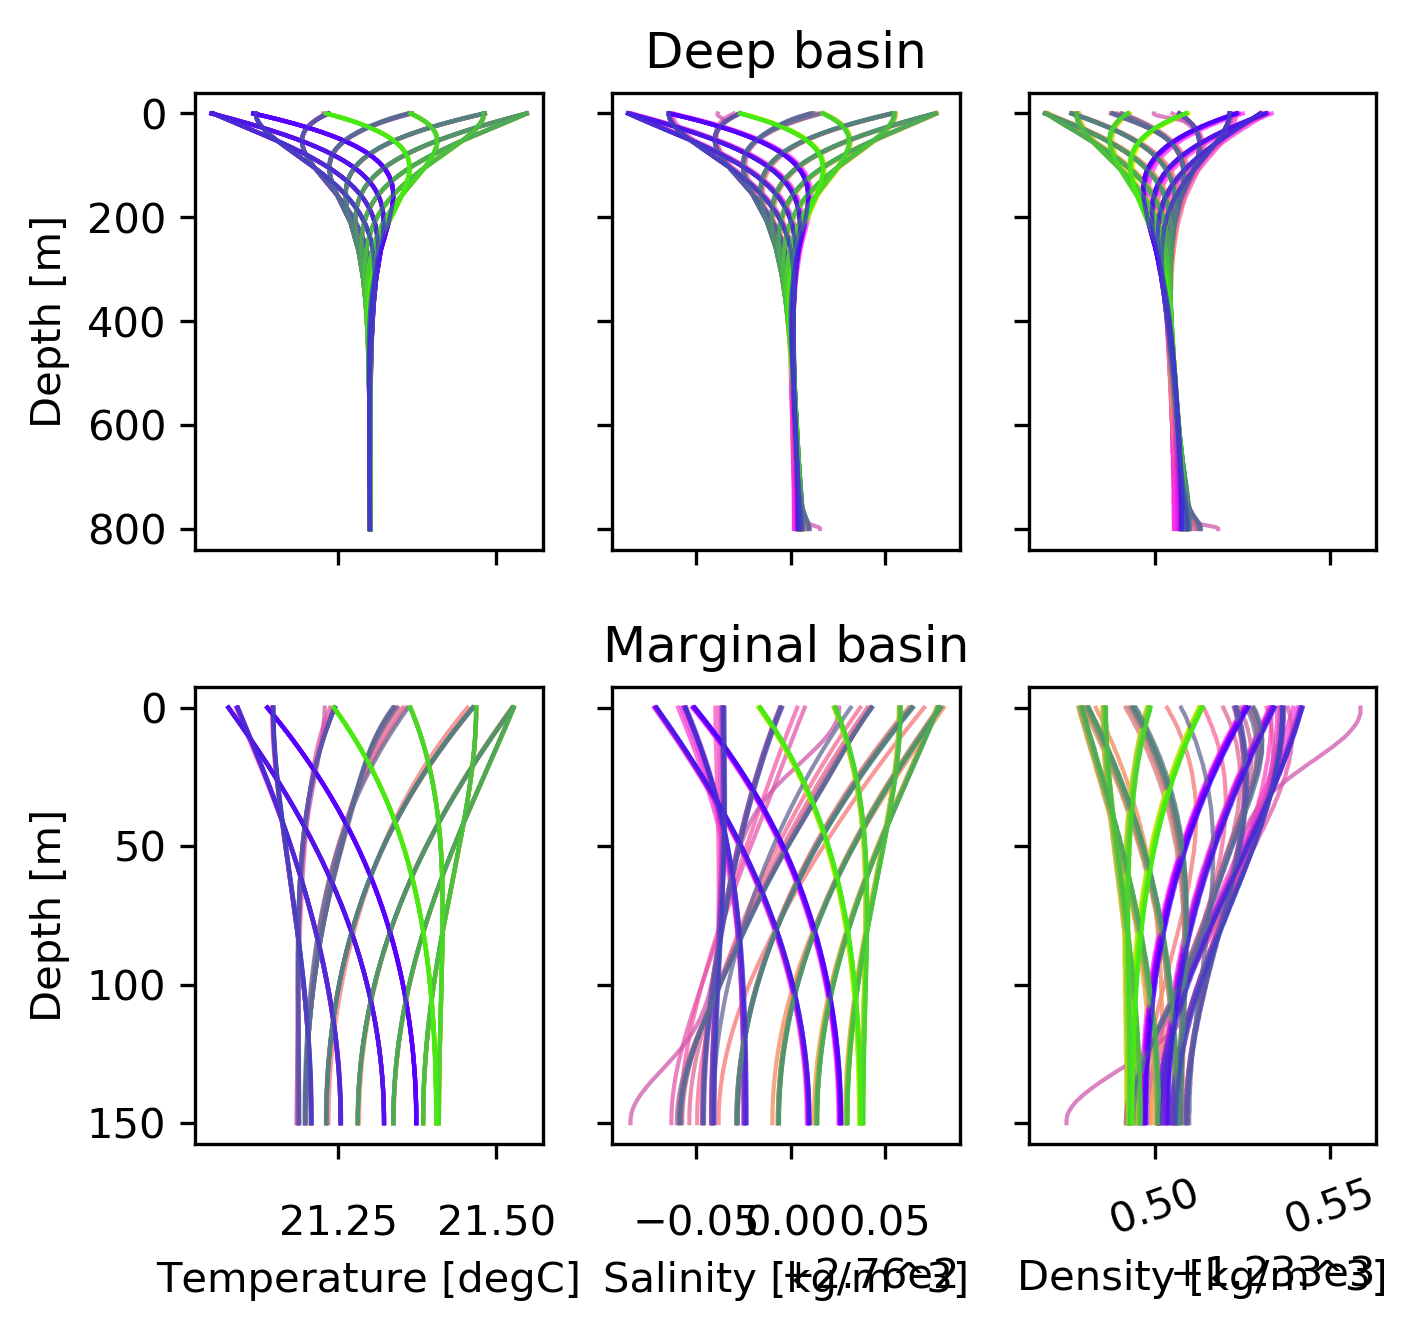
\includegraphics[width=\textwidth,keepaspectratio]{high_bg_diff_kleine_uitslag.png}
\end{subfigure}\hfill
%% subfig 2
\begin{subfigure}[h]{0.20\textwidth}
\centering
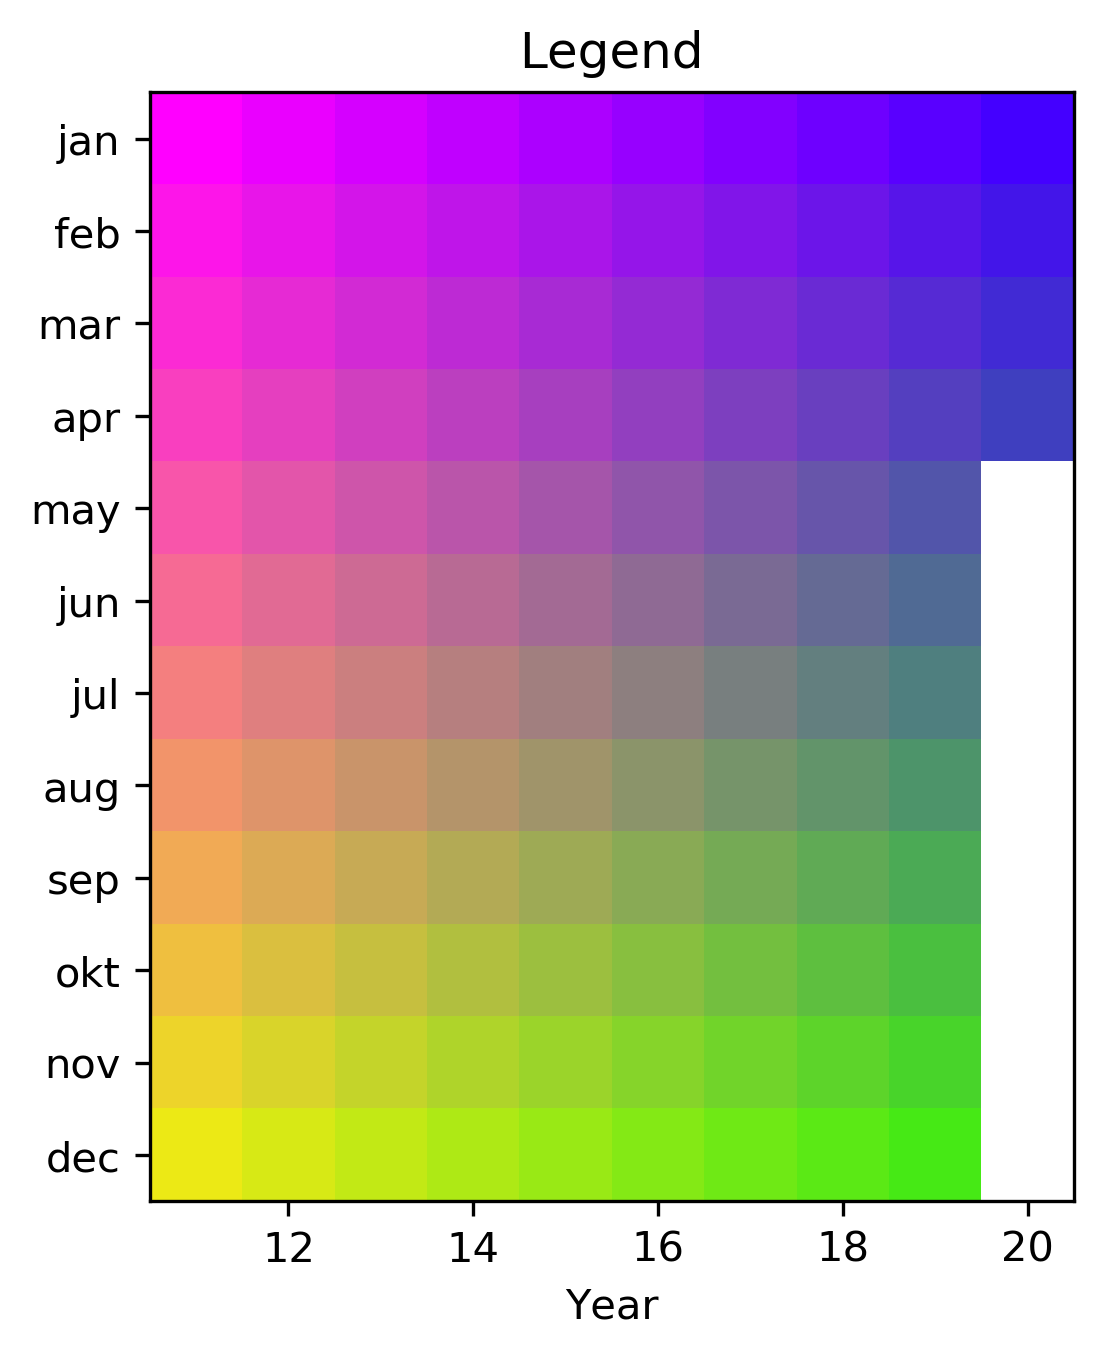
\includegraphics[width=1.0\textwidth,keepaspectratio]{high_bg_diff_kleine_uitslag_Legend.png}
\end{subfigure}\hfill
\caption{Standard model case with advection, a flow of 1e-5 Sv and a marginal basin depth of 150 metres. The background diffusivity was increased, allowing surface processes to penetrate to greater depth}
\label{fig:high_db_success}
\end{figure*}

%% High bg diff MEAN VALUES
\begin{figure*}
\centering
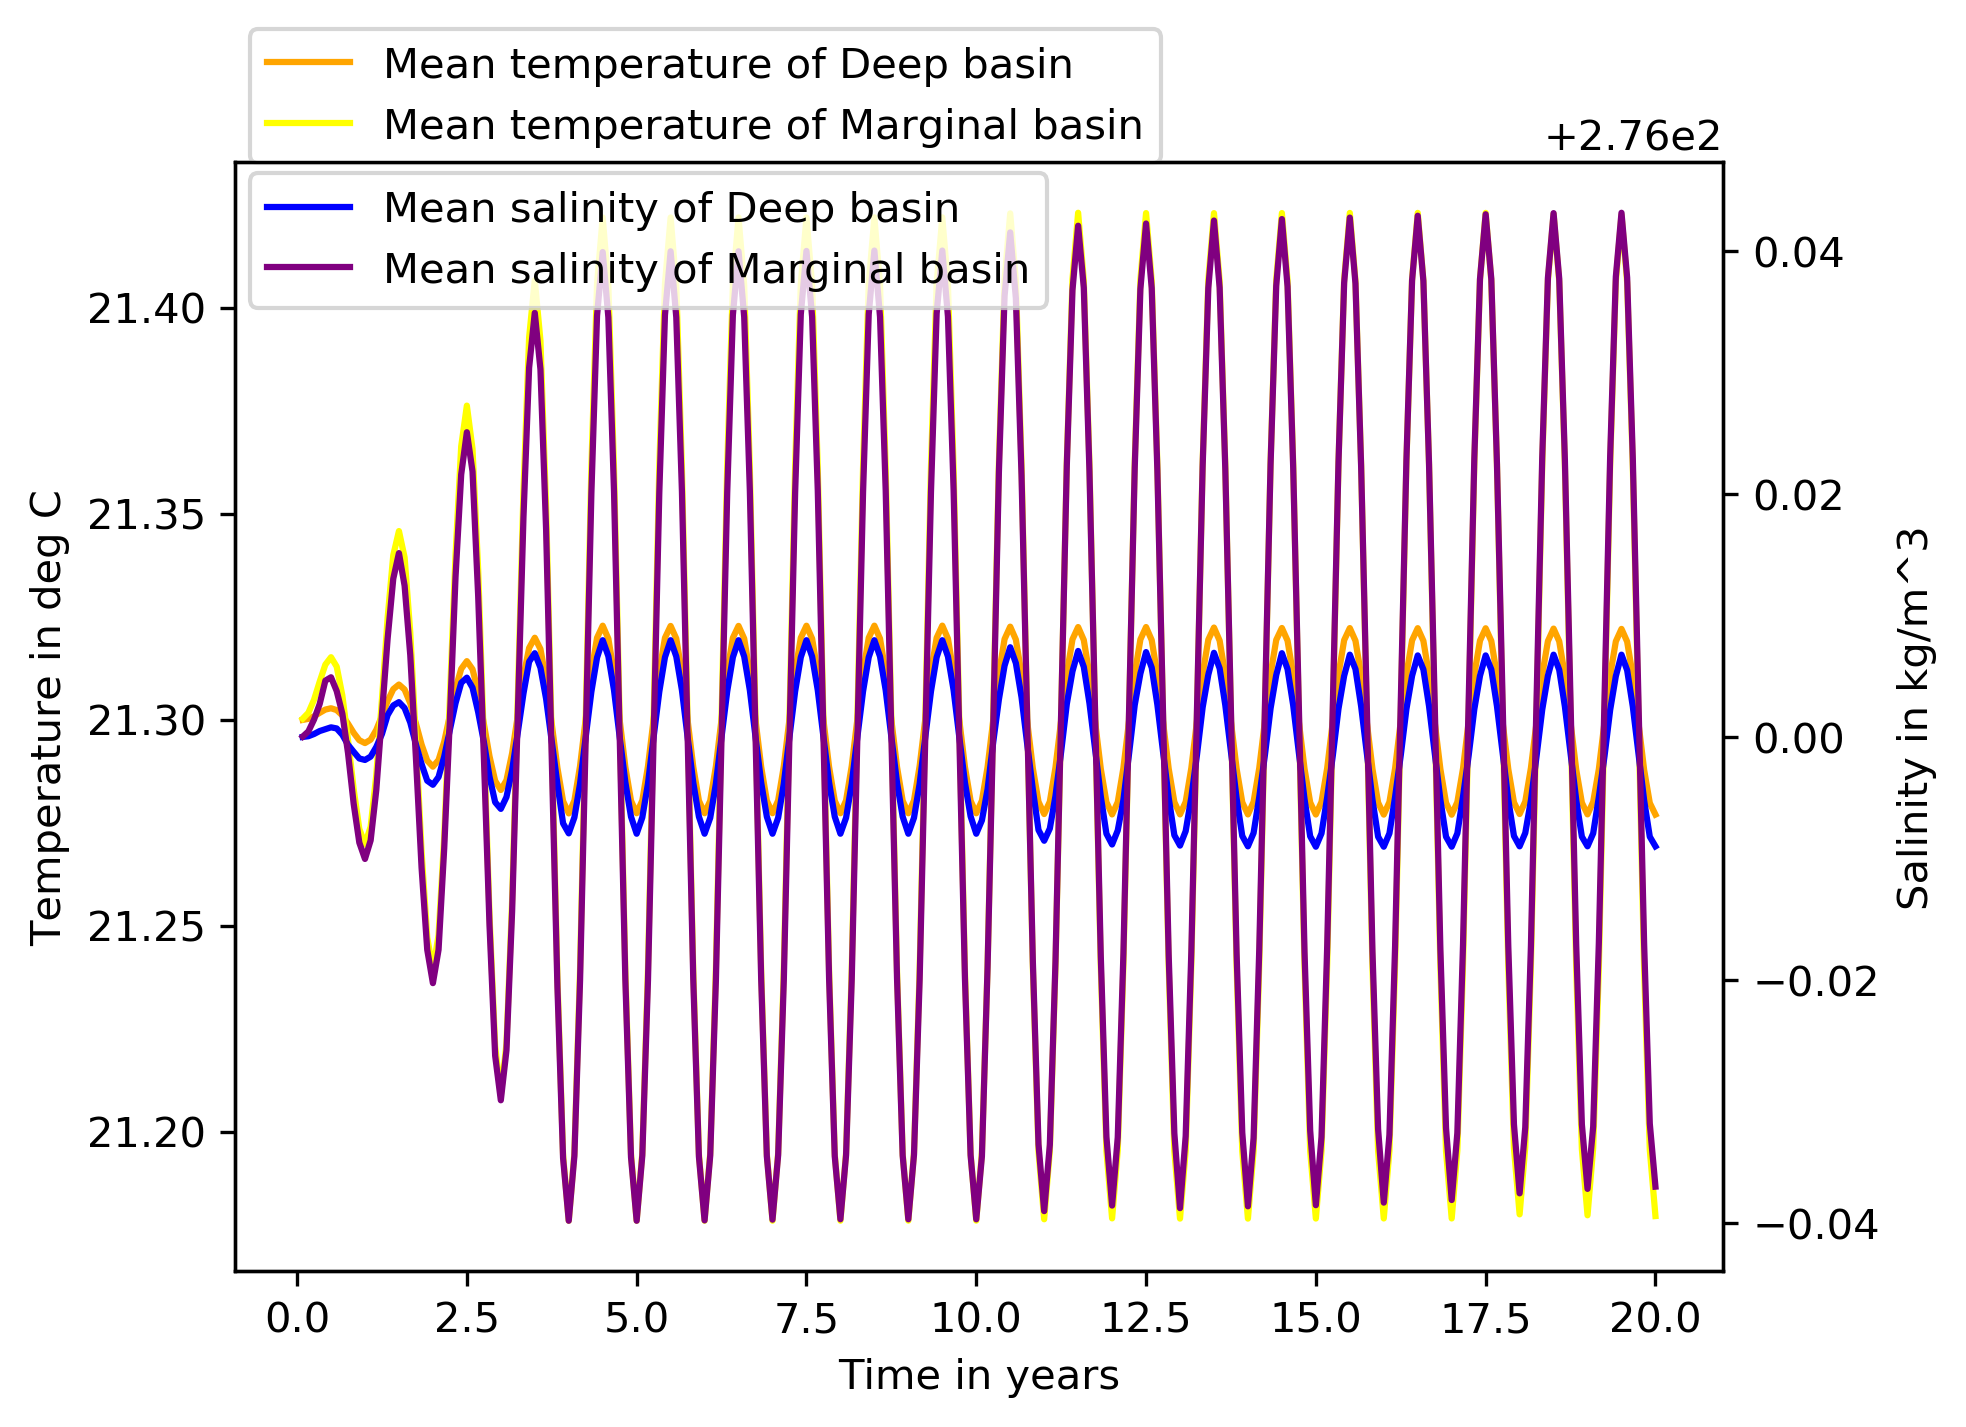
\includegraphics[width=0.9\textwidth,keepaspectratio]{high_bg_diff_kleine_uitslag_mean_values.png}
\caption{Mean values over time corresponding to the scenario shown in figure \ref{fig:high_db_success}}
\label{fig:high_bg_diff_means}
\end{figure*}\hfill


\subsubsection{Net Evaporation}
Figure \ref{fig:high_db_success} shows the results of a standard run and a net evaporation rate resulting in an increase of 0.001 $kg/m^3$ salt per second. The marginal basin yearly increases in salinity as a whole. In the deep basin, the surface and the deep part of the basin increase yearly in salinity as well, with the middle of the column dragging behind.

\subsection{Unintended increases and decreases in the total salt and heat content}
\label{sect:totals_problem}
Figure \ref{fig:hybrid_means} reveals an error in the code, where all averages are increasing even though no net evaporation is active. While increases and decreases may occur in one basin, it should be at the expense of the total amount of the same property in the other basin. However, whenever prolonged periods of continuous advection occur, like in the case shown in figures \ref{fig:high_db_success} and \ref{fig:high_bg_diff_means}, the total amount of salt and heat in the system will be affected.

The two types of column stability check, mentioned in section \ref{sect:stability_methods}, also affect the outcome of this problem. The choice between a whole column check or a bottom up/top down check should be one based on model efficiency and desired detail. Instead, it appears that the total amount of salt and heat in the system systematically increases every year when the whole column check is used, and it systematically decreases every year when the top down/bottom up check is used. The problem effects the salinity more then it does the temperature, though the problem systematically occurs in both. 
The error is smallest when the whole column check is used, which is why this method is used in this research. The effects are however still rather significant when long time spans containing regular exchanging flow are investigated. It was found that the undesired effect is decreased in magnitude when the top and bottom three nodes of the columns are assigned a permanent advection value of zero. It is empirically found that more then three nodes no longer significantly diminish the error. While the error is sometimes decreased by a factor of five using this measure, the root cause of this problem has not yet been discovered so far. 



% % Hybrid fig
% %-------------------
\begin{figure*}
%% subfig 1
\begin{subfigure}[h]{0.7\textwidth}
\centering
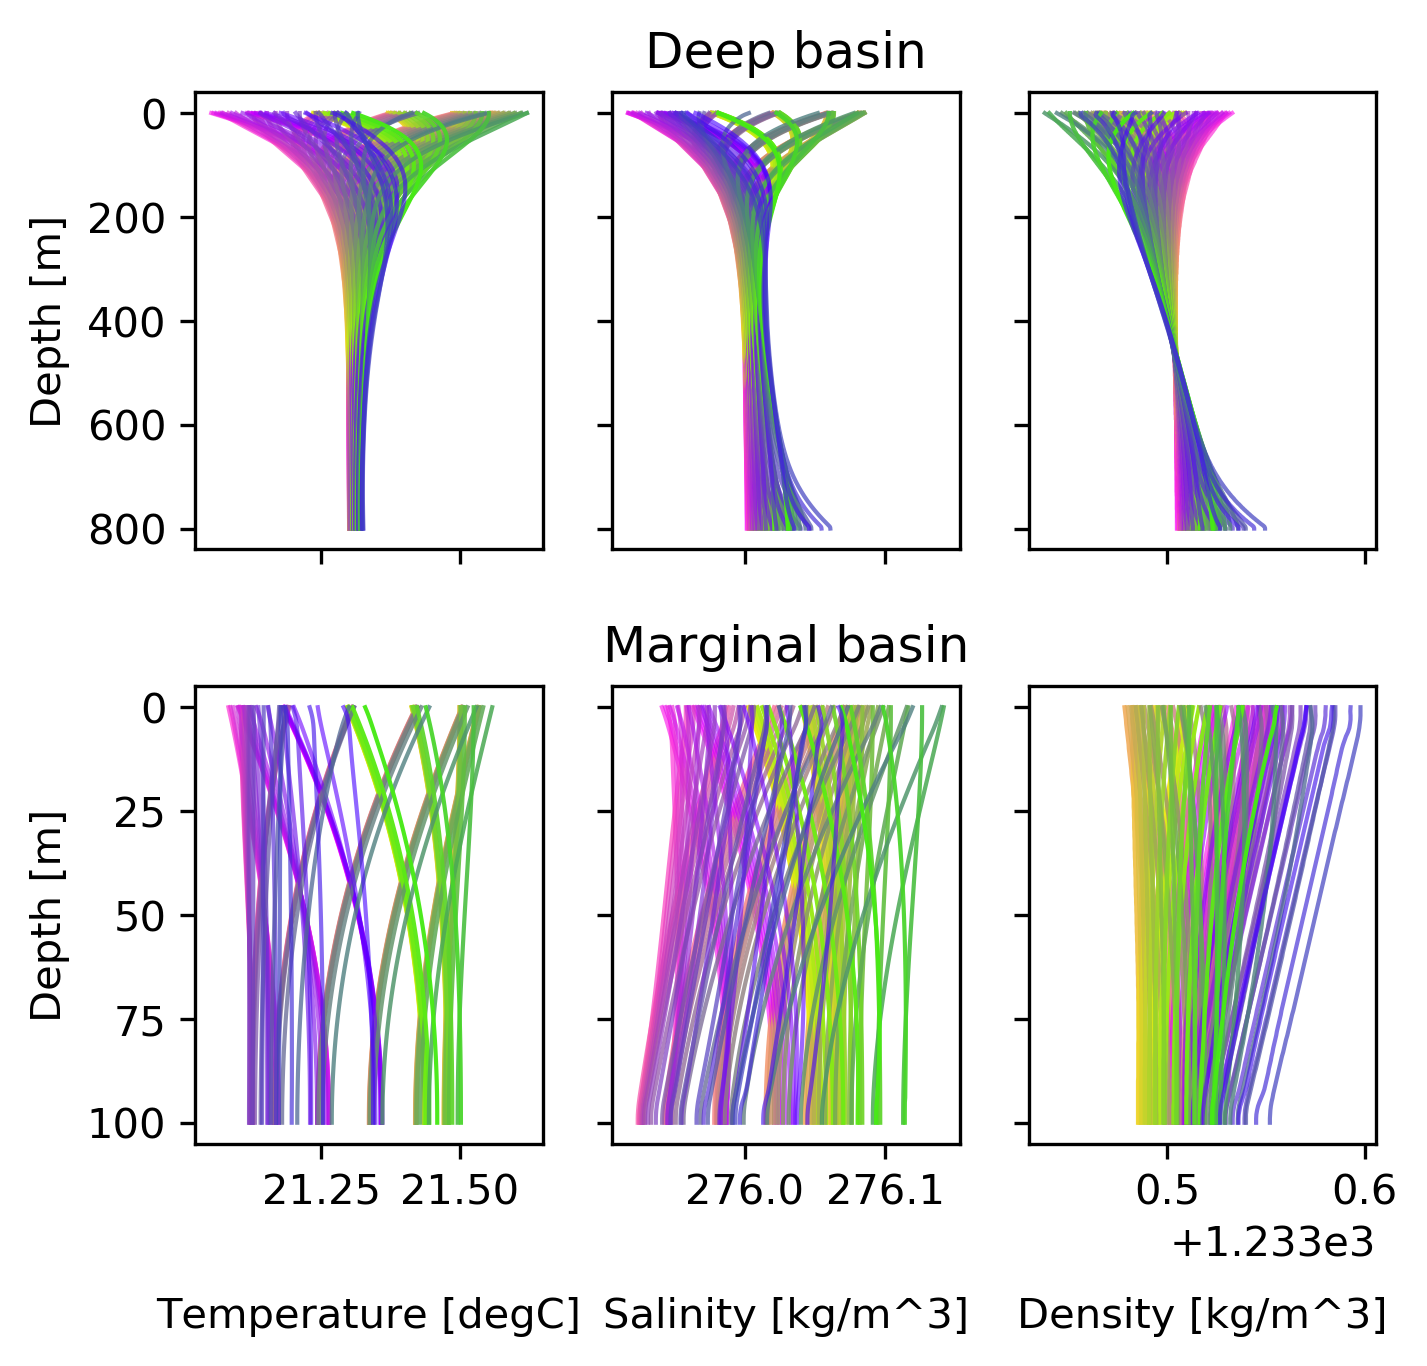
\includegraphics[width=\textwidth,keepaspectratio]{hybrid.png}
\end{subfigure}\hfill
%% subfig 2
\begin{subfigure}[h]{0.20\textwidth}
\centering
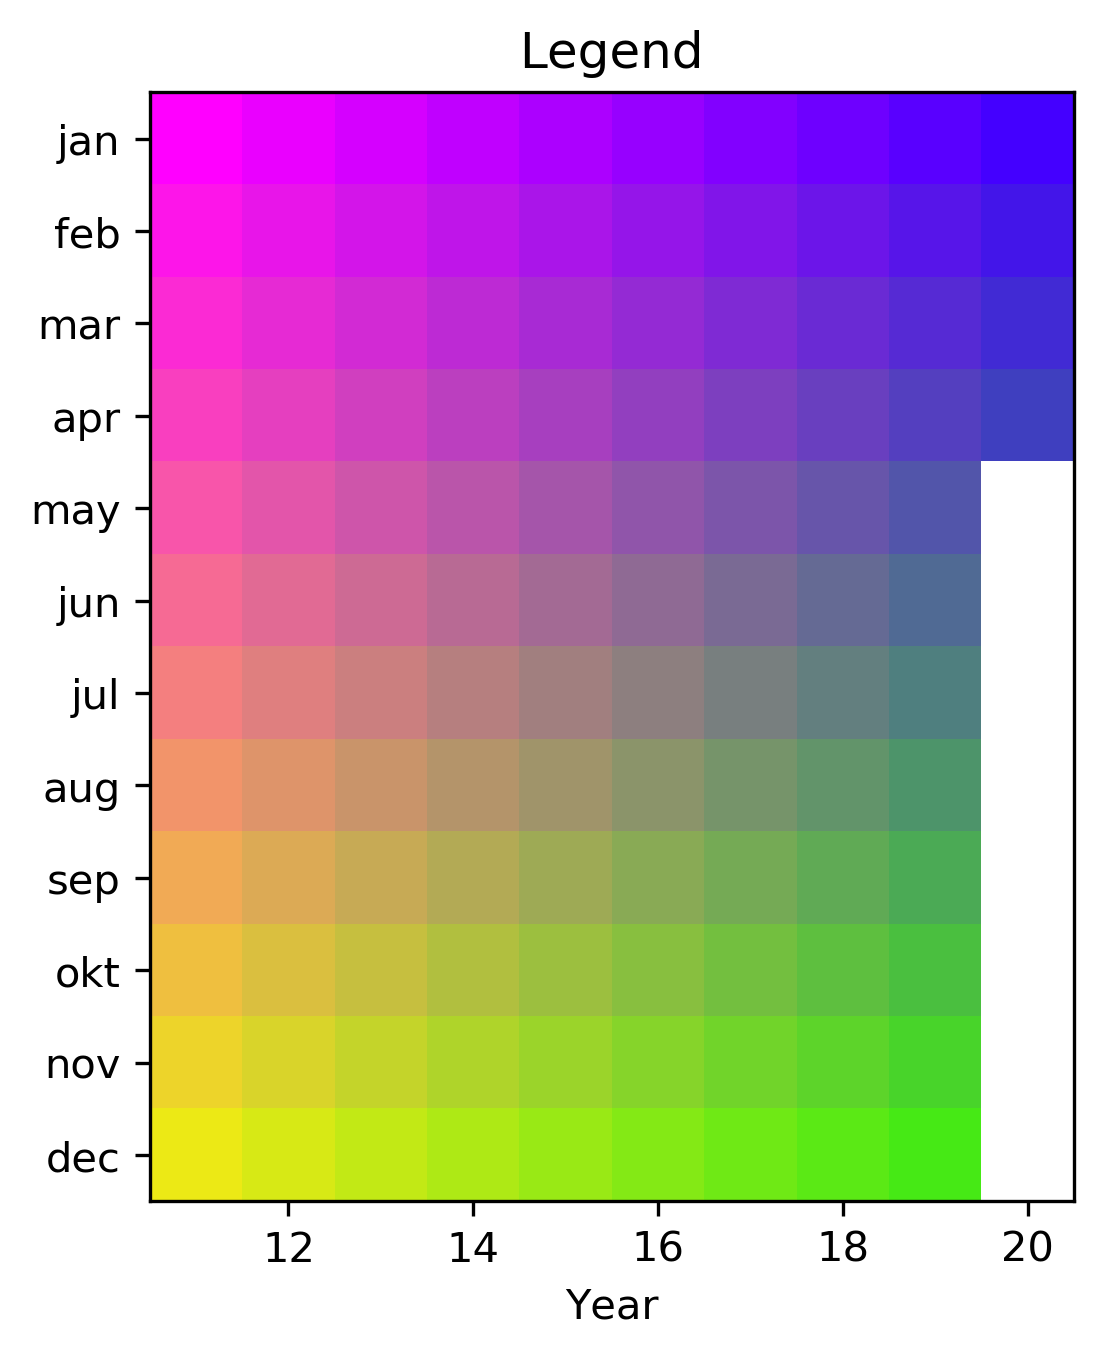
\includegraphics[width=1.0\textwidth,keepaspectratio]{Hybrid_Legend.png}
\end{subfigure}\hfill
\caption{Standard model case with a background diffusivity of 3.0 and a depth of 100m}
\label{fig:hybrid}
\end{figure*}

%% Hybrid MEAN VALUES
\begin{figure*}
\centering
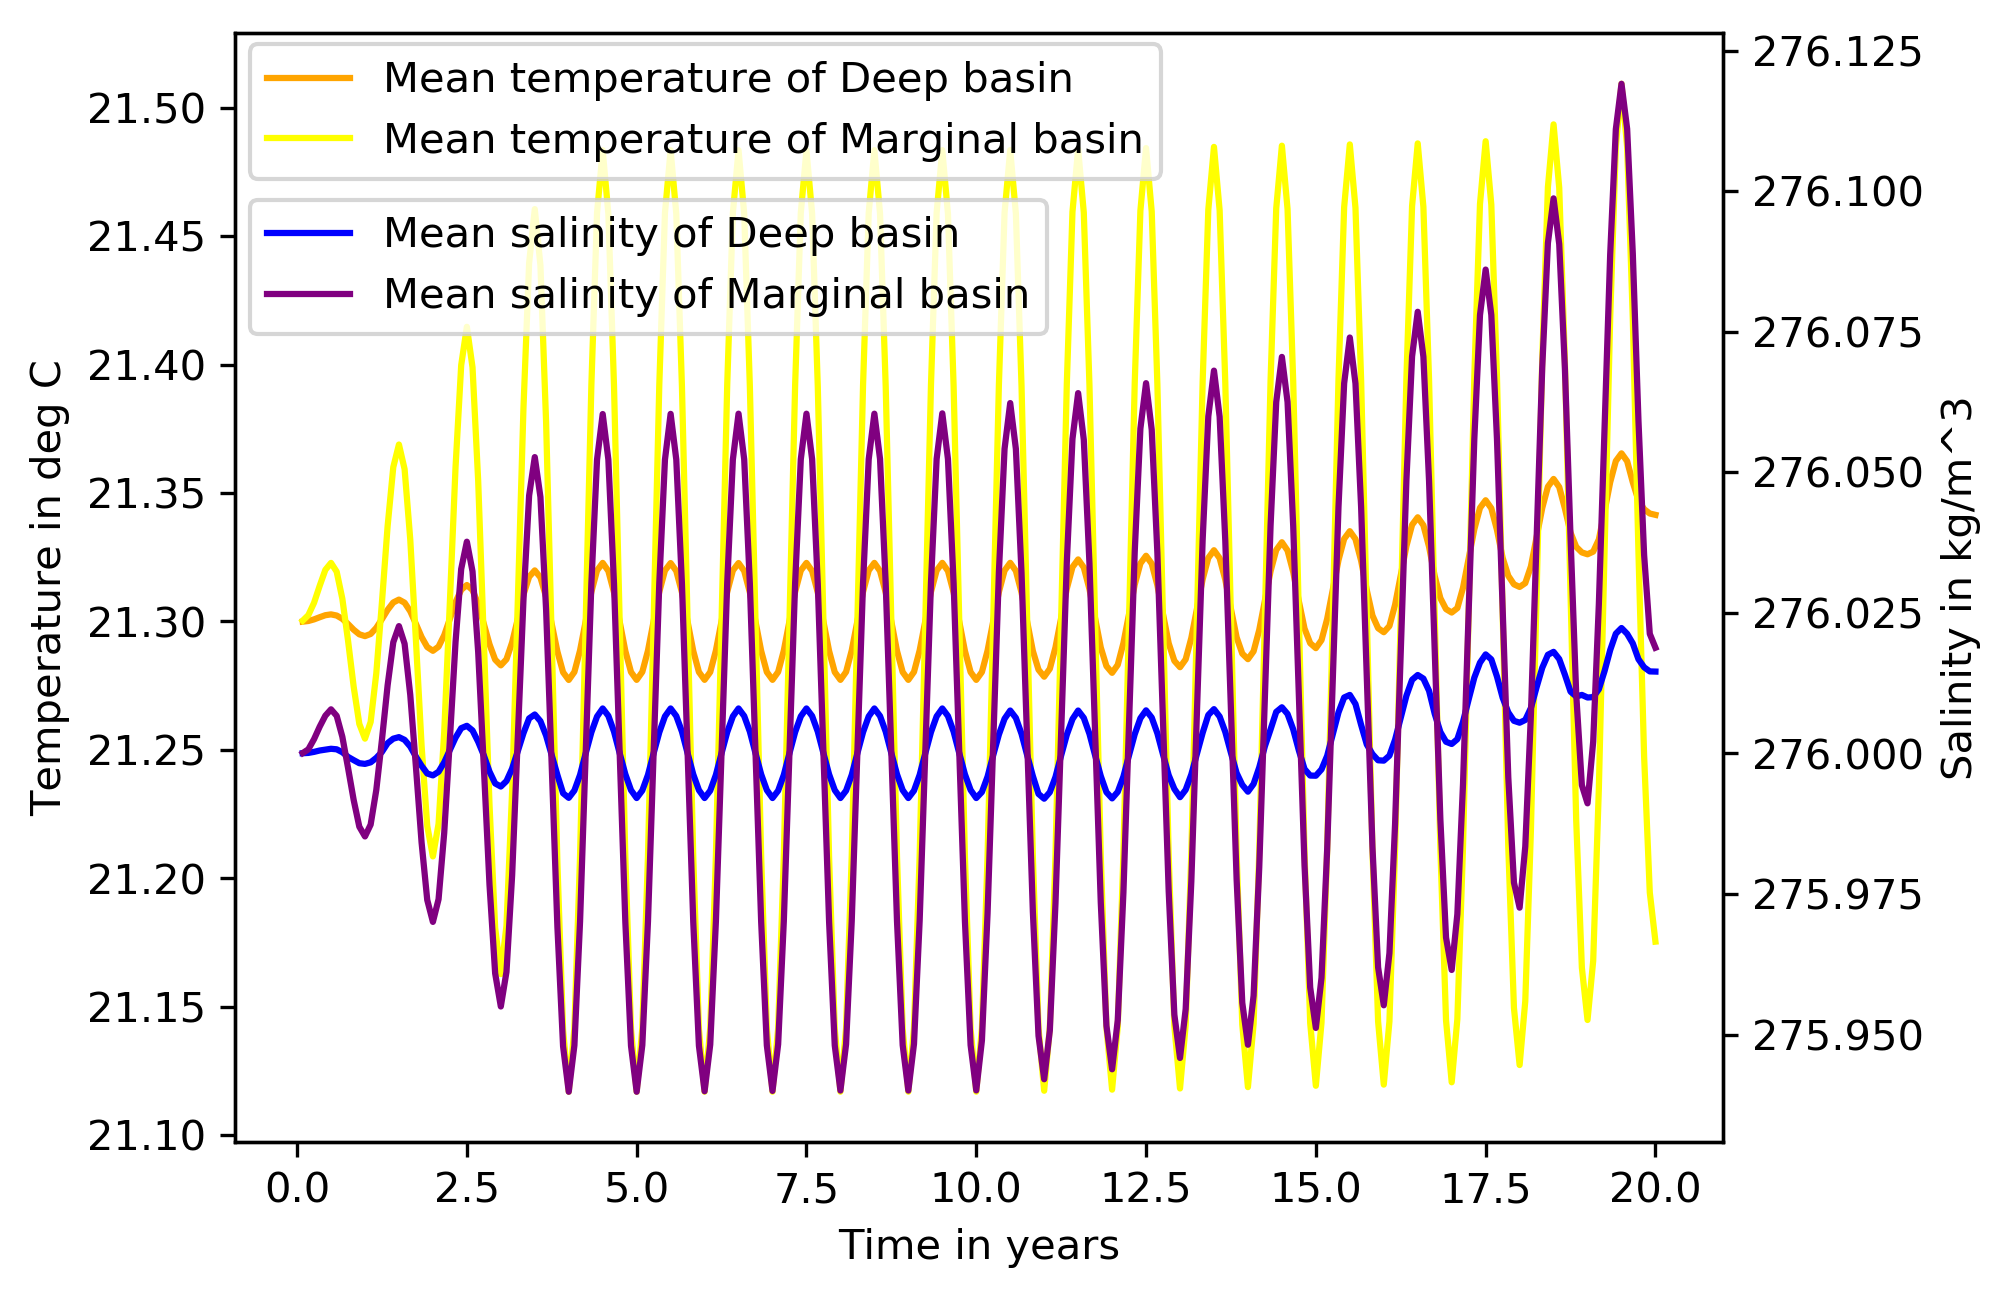
\includegraphics[width=0.9\textwidth,keepaspectratio]{hybrid_means.png}
\caption{Mean values over time corresponding to the scenario shown in figure \ref{fig:hybrid}}
\label{fig:hybrid_means}
\end{figure*}\hfill


%% 0.001 net evap 
\begin{figure*}
%% subfig 1
\centering
\begin{subfigure}[h]{0.70\textwidth}
\centering
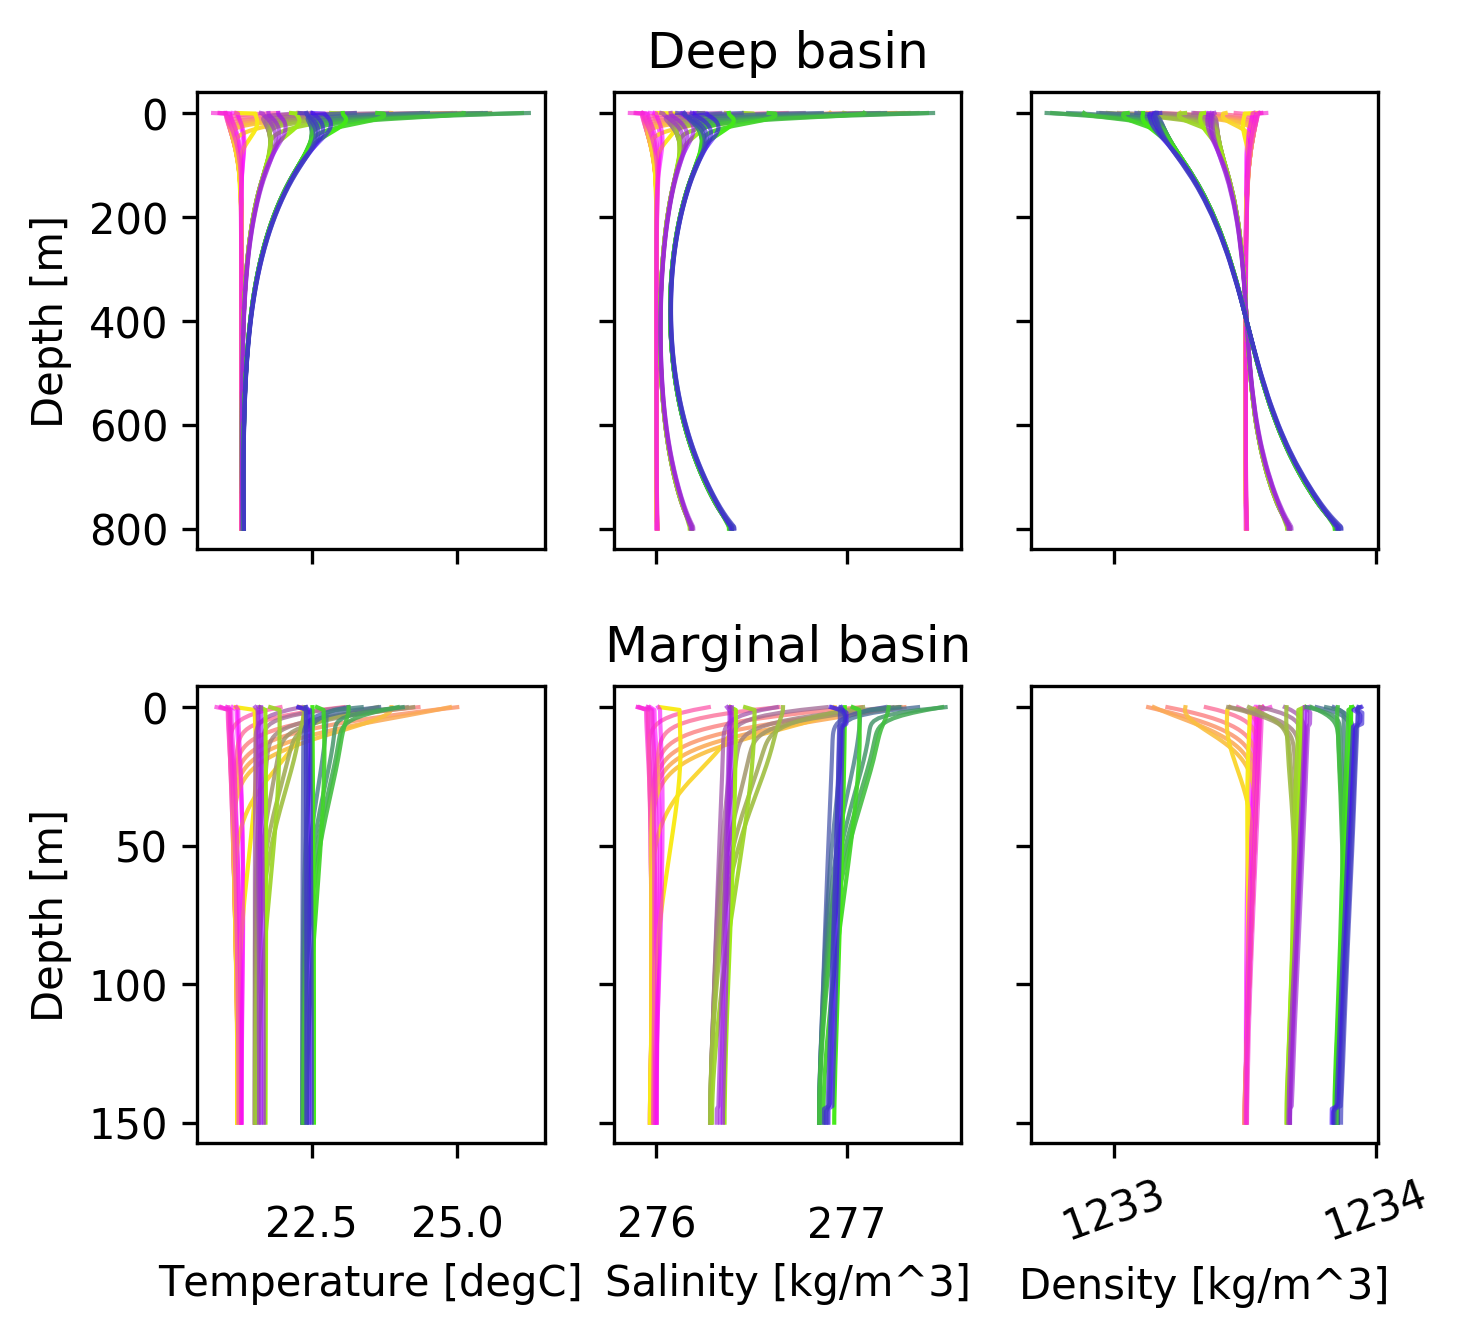
\includegraphics[width=\linewidth,keepaspectratio]{001_net_evap_40yr_3steps_V2.png}
\end{subfigure}\hfill
%% subfig 2
\begin{subfigure}[h]{0.20\textwidth}
\centering
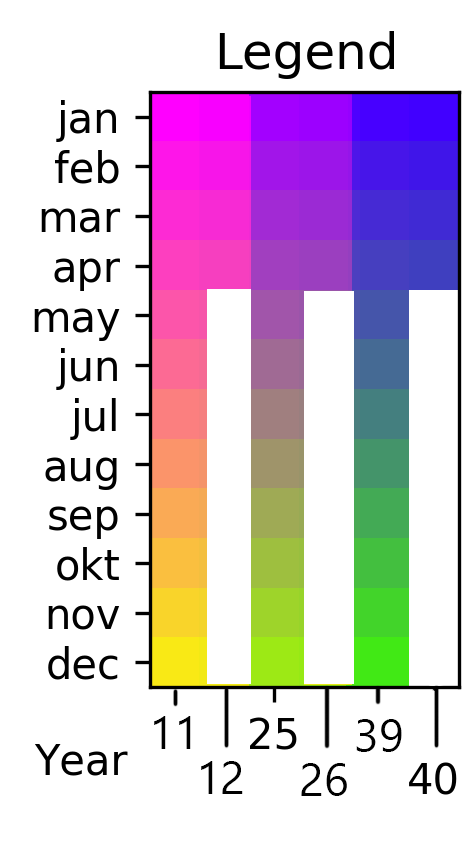
\includegraphics[width=\linewidth,keepaspectratio]{40yr_reduced_Legend.png}
\end{subfigure}\hfill
\caption{Standard model case with a net evaporation rate of 0.001 $kg/m^3$ salt per second.}
\label{fig:net_evap}
\end{figure*}


\subsection{Discussion}
The effects of the surface heat flux and evaporation decrease with depth and can only penetrate down to a maximum depth, the extend of which is determined by the speed of the diffusivity. Shallower basins will therefore experience changes as a result of forcing more quickly and more severely then deeper basins. Increased depth of penetration of surface forcing due to increased background diffusivity goes hand in hand with a reduction in maximum deviation from the mean surface value. When more salt or heat is transported down, there will subsequently be less of it left at the surface. On a similar note, larger background diffusivity more quickly reduces excess salinity in bottom waters.
Neither a significant reduction in marginal basin depth nor a significant increase in background diffusivity resulted in a pronounced increase in salinity in the bottom of the deep basin. The combination of the two measures did accomplish this. Alternatively, very extreme variants of the two individual cases are also capable of producing saline deep basin bottom waters.

When the evaporation is significantly higher than the influx of fresh water, the whole column will become more saline. This has a larger effect on the marginal basin, for it contains a smaller volume of water. This large effect on the evaporation on the salinity and, by extension, density of the marginal basin results in a yearly increase in the salinity at the bottom of the deep basin. The density of the marginal basin as a whole very directly follows the density at the bottom of the deep basin. While the surface and bottom of the deep basin are increasing rapidly in salinity almost as a direct result of the net increase, the rate of increase in salinity in the middle of the deep basin is limited by the rate of background diffusivity.

An expected result of the net evaporation was that the marginal basin would be nearly permanently mixing. During winter the columns are unstable due to the cooling, as is the case with most other model output in this report. During summer, the increased overall evaporation would then have resulted in extra saline surface waters, creating instability during summer not unlike that described in section \ref{sect:Summer_mixing_discussion}. However, the net surface temperature is also increasing (figure \ref{fig:net_evap}) which counteracts the possibility of mixing in summer. This significant increase in surface temperature was unexpected and is currently thought to either be a result of the density dependence of the heat forcing or a result of the problem discussed in section \ref{sect:totals_problem}. This phenomenon has not yet sufficiently been investigated and is a point of consideration for future studies building on this research.


While the combination of an increased background diffusivity and a decreased marginal basin depth resulted in a significant excess salinity in the bottom of the deep basin, the salt in the system can only be re-distributed. This puts an upper limit to the amount of excess salinity the bottom waters can hold. Net evaporation does not have this restriction and therefore seems to be a mechanism that is more capable of inducing significant halite precipitation from a deep brine in the long term.

\subsubsection{Equilibrium}
Every year flow takes place that increases salinity in the bottom of the deep basin by a slight amount, salt is added to and extracted from the bottom of the deep and marginal basins, respectively. The reverse occurs near the surface of the basin. The redistribution of salt from and towards these extremes through diffusion creates a linear profile over time, the slope of which is mainly dependent on the background diffusivity. This inclination towards a linear profile over time can best be observed in figure \ref{fig:high_db_success}. The linear dependence of the slope $\frac{\delta Q}{\delta t}$ on the diffusivity can also be observed directly from equation \ref{eq:diff_original}. This equation shows a similar relation between the slope and the advection, but the advection is generally about two orders of magnitude smaller then the background diffusion. Also, advection only occurs in periods of exchanging flow as opposed to the continuous presence of the background diffusivity. 
This equilibrium seems to be determined by the difference, or eventual lack thereof, in salinity between the top and the bottom of the deep basin. The equilibrium is theoretically reached when the yearly maximum salinity in the bottom of the deep basin is roughly similar to that in the bottom of the marginal basin. The marginal basin will then reach a stable yearly average density, capping any further growth of the deep basin brine. No solid conclusions can be made on the long term outcome of the model however, for as of yet unidentified imperfections in the code have undesired effects on the total salt and heat contents in the basins, as discussed in section \ref{sect:totals_problem}.

\subsubsection{The cycle of exchanging flow}
\label{sect:flow_cycle}
The large pulse of flow marked as (1) in figure \ref{fig:with_adv_large_effect} occurred in January after which no more flow was exchanged the following years. This is rather different in a scenario where the flow occurs gradually rather then pulse-wise. In all four scenarios (figures \ref{fig:Very_shallow_basin}, \ref{fig:high_db_success}, \ref{fig:hybrid} and \ref{fig:net_evap}) the exchanged volume is rather minor. In these scenarios the flow between the basins also starts in winter. The months differ slightly per scenario but the process is the same. As the winter is progressing, the marginal basin is continuously cooling and thus increasing in density. From April onward, the column is also increasing in salinity due to the increasing evaporation in spring. In the marginal basin the effect is increased since the exchanging flow still continues and the surface water that is entering the marginal basin now is warmer and more saline then the deeper water leaving it. The increase in temperature and by extension the effect it has on the density is however rather small when compared to the increase in salinity. The marginal basin is still in an unbalanced state due to the saline surface water so mixing in the marginal basin is quick in resupplying salt to the bottom. Since the exchanging flow from the marginal basin to the deep basin is now more saline then in winter, the salinity of the bottom waters of the deep basin increases rapidly during spring. In the end of spring/beginning of summer, the turning point is reached, where the marginal basin is now too warm and the bottom water of the deep basin too dense to allow further exchanging flow. 
During the summer and fall, salt diffuses up from the saline bottom waters in the deep basin, thereby slowly reducing its salinity. During the fall, the marginal basin is cooling again, increasing its density. At the start of winter, the density of the marginal basin has increased enough and the density of the bottom water of the deep basin has decreased enough to again allow for exchanging flow. However, the bottom waters of the deep basin have not yet lost all of their salt since the previous exchange, for the background diffusivity is slow. Since significantly more water enters the marginal basin then leaves it during every spring, the deep bottom water is expected to slightly increases in salinity every year and the surface water of the deep basin is expected to decreases in salinity every year, until the near equilibrium is reached. The marginal basin is expected to be more strongly influenced by this exchange, for it has a smaller volume. The effect is however not visible in the data, either because the effect is too small to make a visible impact but most likely, since it only occurs in periods of exchanging flow, it is overshadowed by the problem discussed in section \ref{sect:totals_problem}.

% While the expected effect does occur, the deep salt layer is rather small. Larger flow does create a more pronounced deep salt layer, but this would be one that is more saline then the bottom of the marginal basin was at the time of flow, which could not happen in reality. Less flow between the basins makes for a rate of increasing salinity at the bottom of the deep basin that is gradual enough to allow for diffusion and advection in the deep basin to negate the effect. Next to no saline bottom layer would form in the deep basin. Also, figure \ref{fig:Very shallow_basin} was created with the two basins having an equal surface area. When the deep basin is made larger, no visible change occurs in the deep basin for the salt is distributed over too large and area to be of significance. If the marginal basin is made too small, the model can reach some threshold from where the results are nonsense, as discussed in section \ref{sect:adv_problem}.

% The effect was expected to be well pronounced, but the results indicate that decreasing the depth of the marginal basin on its own does not yield a significantly saline bottom layer in the deep basin. 

% \label{sect:shallow_basin_issue}
% In shallow basins, the forcing is dominant in a large part of the column when compared to deeper basins, which is fully expected for both columns are subject to the same diffusivity. Figure \ref{fig:Very shallow_bains_issue} however, shows an unforeseen decrease in both the temperature and salinity. Since the decrease in temperature is faster then that of the salinity, the density keeps increasing. This decrease in salinity and temperature is a consequence of the low amount of total salt and heat stored in the shallow column. Changes in salt content and total heat now have a pronounced effect. In this case, the change in total salt and heat content can be due to two factors. The first option is the flow between columns where the marginal basin loses more then it gains, as discussed in section \ref{sect:SS_&_adv}. The second option is a net loss of salt and heat during mixing in winters. Since the diffusion is set higher then    %%CONTINUE HERE about fig \ref{fig:Very shallow_bains_issue}  DOES THIS ONLY HAPPEN WITH HIGH ADV??

% Figure \ref{fig:with_adv_large_effect_145m} was run with a marginal basin that is only slightly more shallow then that of figure \ref{fig:with_adv_geen_uitslag} and has a significantly lower connective flow. 

% \subsection{The advection problem}
% \label{sect:adv_problem}
% The code yields unrealistic results under certain input parameters. This generally involves one or both basins continuously either increasing or decreasing in both salt content and heat content to unrealistic values such as negative numbers or several times the starting amount. This can occur even if there is no net evaporation. Primarily this goes wrong if the marginal basin is very small in surface area and depth and $U_{lat}$ is high. What may be occurring is that high advection (dependent on the amount of flow between the basins and the surface area of the basin) can cause salt and heat to be leaked or added at the boundaries. That this effect generally happens in shallow marginal basins may be due to the flow and advection re-occurring every year in continuous periods, continuously adding or subtracting at the boundaries as opposed to once every few years in a pulse. 

% A workaround is found by forcing $U_{lat}$ to be zero in the top and bottom nodes. The higher $U_{lat}$, the more pronounced the issue becomes and the more nodes need to be forced to zero. No proper solution has been found so far. 




% \pagebreak
% \subsection{Background diffusivity}
% The effects that result from increasing background diffusivity is expected to be similar to the results yielded by a shallower marginal basin. In both cases, variations created at the surface due to forcing will reach the bottom of the marginal basin sooner.

% \subsubsection{Results}
% Figure \ref{fig:high_db_success} resembles figure \ref{fig:Very_shallow_basin} rather closely in form. The same transition from a vertical to a diagonal profile is present. A few aspects vary between the images like the depth to which the surface forcing penetrates and the maximum deviation from the average temperature at the surface. 




% \subsubsection{Discussion}
% The depth of penetration of surface forcing goes hand in hand with a reduction in maximum deviation from the mean surface value. When more salt or heat is transported down, there will subsequently be less of it left at the surface. 

% However, where the increase in salt and heat content in the marginal basin decreased over time in section \ref{sect:mar_basin_depth}, here it increases with time. This is due an unintended artificial increase in salt content as described in section \ref{sect:totals_problem}.  
 

% \subsection{Net Evaporation}


% \subsubsection{Results}






%%%%%%%%%%%%%%%%%%%%%%%%%%%% Results

% \section{Results}
% Output of the simplest version of the code will be presented first.  Thereafter, output of the code with convection will be shown, as well as output influenced by the source-sink and advection terms. After the impacts of the individual features are shown, the influence of several parameters on the outcome will be presented. \todo{Is this still necessary with new layout?}



% \subsection{Source sink and advection}
% % Wrap-Fig Legend for discuss adv and Fig SS
% %----------------------------------------
% A typical result of the model but with no advection is shown in figure \ref{fig:no_adv}. In this figure, we see mixing of part of the column in October and November and whole column mixing from December to March, best visible in the temperature plots. The density distribution in the deep basin is fully stable while that in the marginal basin is mixing regularly and four distinct episodes can be recognized.
% In a case with advection, the dense water body at the bottom of the deep basin shows to generally be a lot less pronounced or not present at all, like in figure \ref{fig:with_adv_geen_uitslag}. In figure \ref{fig:with_adv_large_effect}, a model run with advection and a flow of 40 Sv is shown. This way, we can analyze the workings of the code, for the effects are large enough to see in the figure. This figure is discussed in section \ref{sect:large_effect}. In both advection cases, the marginal basin shows no distinct episodes where salt is resupplied to the bottom as is seen in figure \ref{fig:no_adv}.

% % Fig SS
% %-------------------
% \begin{figure*}
% %% subfig 1
% \begin{subfigure}[h]{0.77\textwidth}
% \centering
% \includegraphics[width=\textwidth,keepaspectratio]{"no adv good".png}
% \end{subfigure}\hfill
% %% subfig 2
% \begin{subfigure}[h]{0.23\textwidth}
% \centering
% \includegraphics[width=\textwidth,keepaspectratio]{"no adv good Legend".png}
% \end{subfigure}\hfill
% \caption{Model run with source-sink and no advection. The situation shown is right after flow between the two basins occurred.}
% \label{fig:no_adv}
% \end{figure*}

% % Fig with adv, geen uitslag onderaan
% % Had :
% % flowdepth=		5
% % strait_depth= 		500.
% % strait_width= 		6000
% % U_lat= 			0.001
% % width_basin1:		  15000.
% % width_basin2:		  5000.
% % length_basin1=        80000 
% % length-basin2=        80000
% %
% % Salt_diff_amplifier=	1
% % Temp_diff_amplifier=	1.
% % evaporation_amplifier1= 0.3
% % evaporation_amplifier2= 0.3
% % mean_evap_rate=         0.0
% %-------------------
% \begin{figure*}
% %% subfig 1
% \begin{subfigure}[h]{0.8\textwidth}
% \centering
% \includegraphics[width=\textwidth,keepaspectratio]{with_adv_geen_uitslag_onderaan.png}
% \end{subfigure}\hfill
% %% subfig 2
% \begin{subfigure}[h]{0.20\textwidth}
% \centering
% \includegraphics[width=\textwidth,keepaspectratio]{with_adv_geen_uitslag_onderaan_Legend.png}
% \label{fig:}
% \end{subfigure}\hfill
% \caption{Model run with advection. The same input parameters as the run shown in figure \ref{fig:no_adv} were used.}
% \label{fig:with_adv_geen_uitslag}
% \end{figure*}


% % % Fig with adv, ook uitslag onderaan
% % %-------------------
% % \begin{figure*} 
% % \centering
% % \includegraphics[width=1\textwidth,keepaspectratio]{"with adv good".png}
% % \caption{Model run with advection. A color legend is shown in figure \ref{fig:legend}.}
% % \label{fig:with_adv}
% % \end{figure*} \todo{mention why basin is so shallow}

% % % Fig with adv, grote uitslag, genummerd
% % %-------------------
% \begin{figure*}
% %% subfig 1
% \begin{subfigure}[h]{0.8\textwidth}
% \centering
% 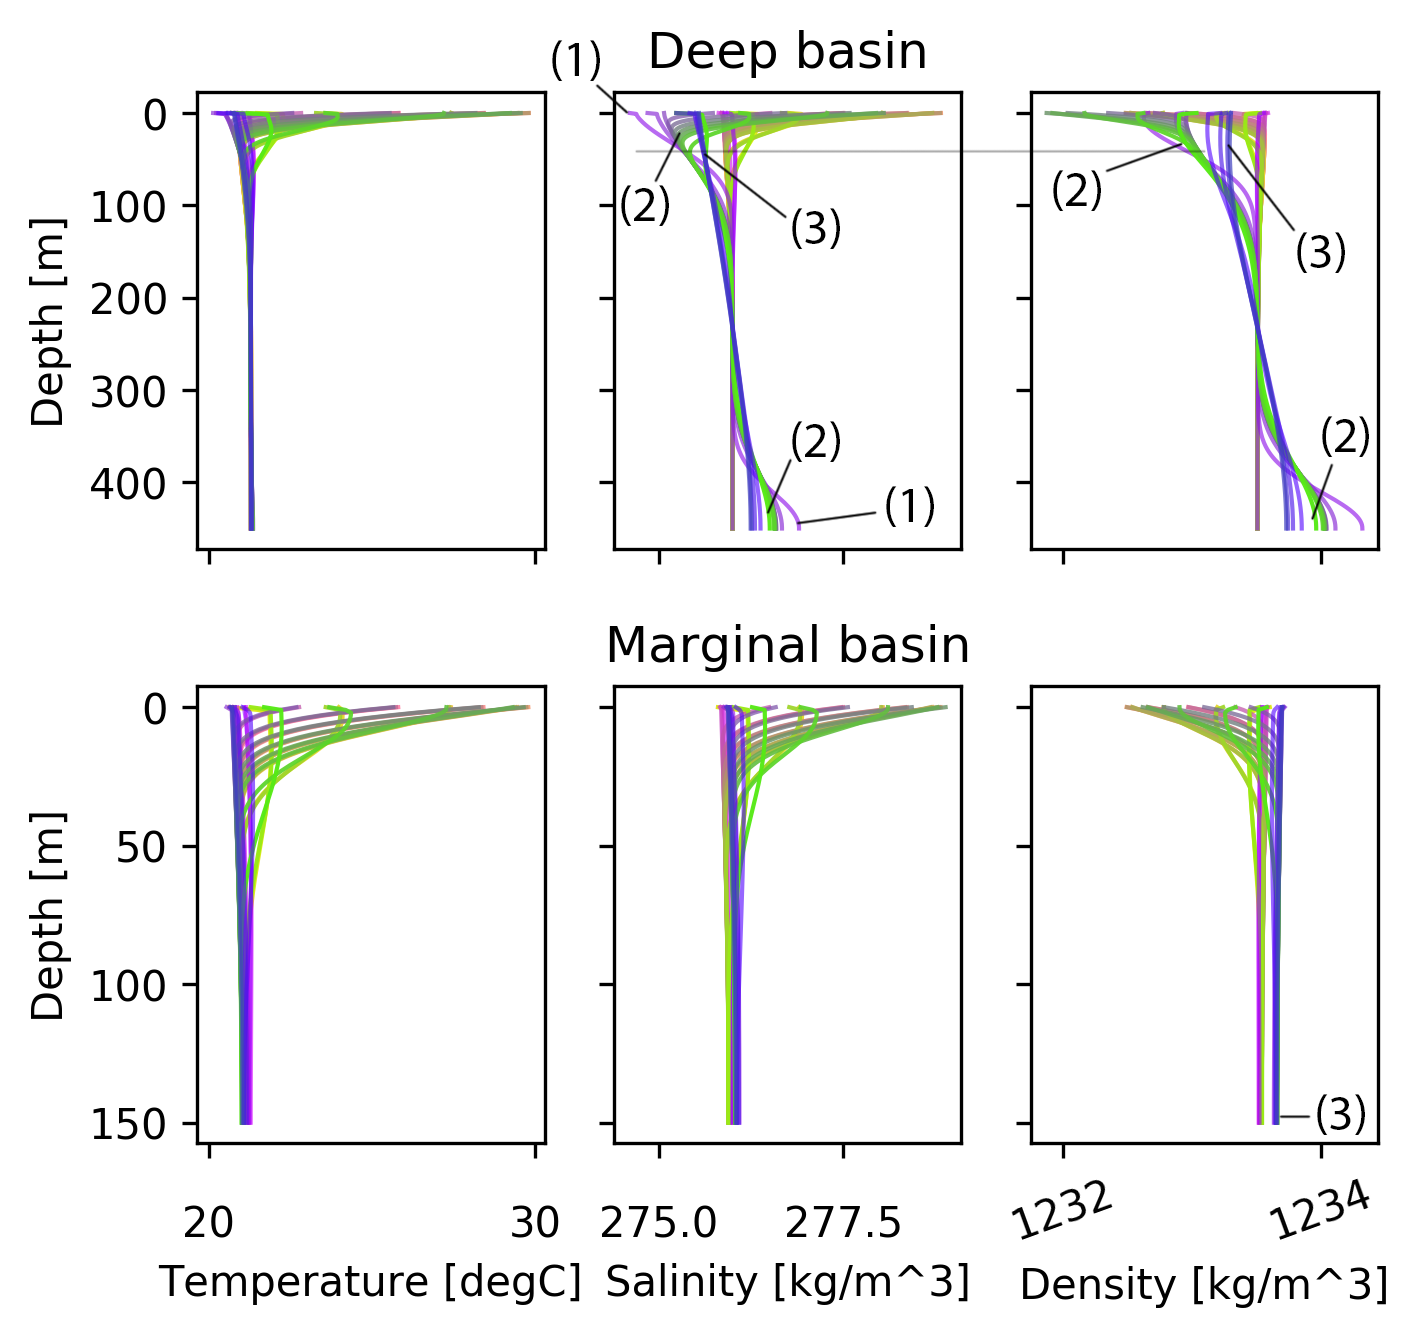
\includegraphics[width=\textwidth,keepaspectratio]{with_adv_large_effect_40SV_altered.png}
% \end{subfigure}\hfill
% %% subfig 2
% \begin{subfigure}[h]{0.20\textwidth}
% \centering
% 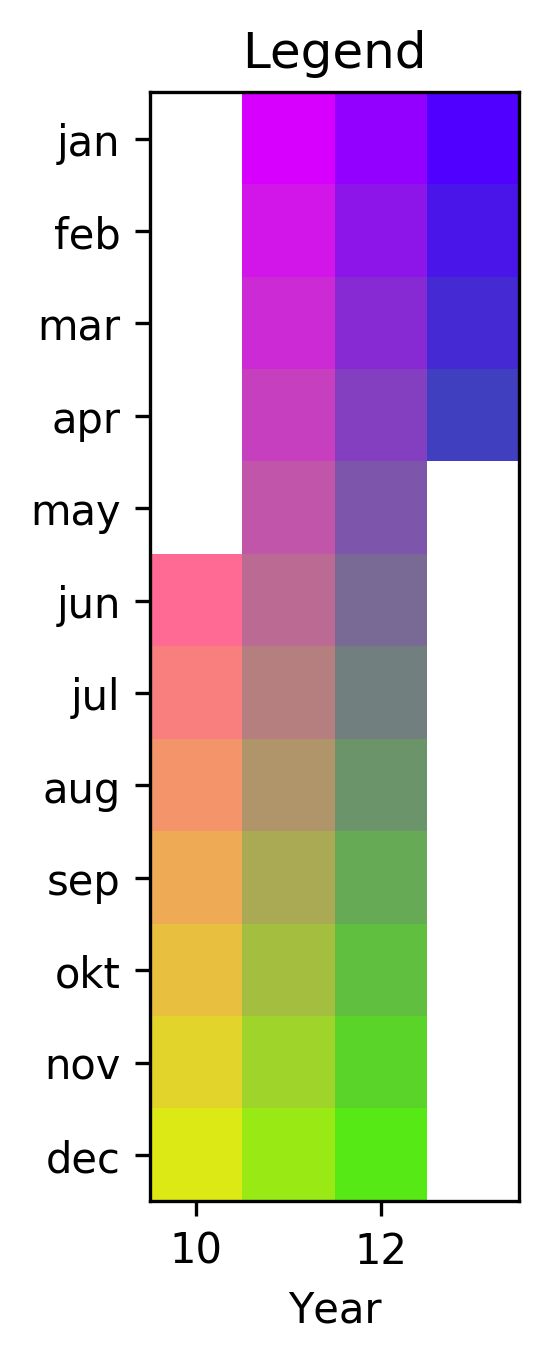
\includegraphics[width=1.0\textwidth,keepaspectratio]{with_adv_large_effect_40SV_Legend.png}
% \end{subfigure}\hfill
% \caption{Model run with advection. (1): initiation of the exchanging flow (2): slow decrease of anomaly (3): mixing. }
% \label{fig:with_adv_large_effect}
% \end{figure*}


% \subsection{Parameter variations}

% \subsubsection{Basin depth}
% Figure \ref{fig:Very shallow_bains_issue} shows the results of a run with all features and a 50m deep marginal basin. The flow creates mere slight disturbances in the deep basin. In the marginal basin however, both the temperature and salinity decrease every winter to unrealistic values. When given enough time, the temperature will reach negative values. This issue is further discussed in section \ref{sect:shallow_basin_issue}. BLA

% \begin{figure*}
% %% subfig 1
% \centering
% \begin{subfigure}[h]{0.80\textwidth}
% \centering
% 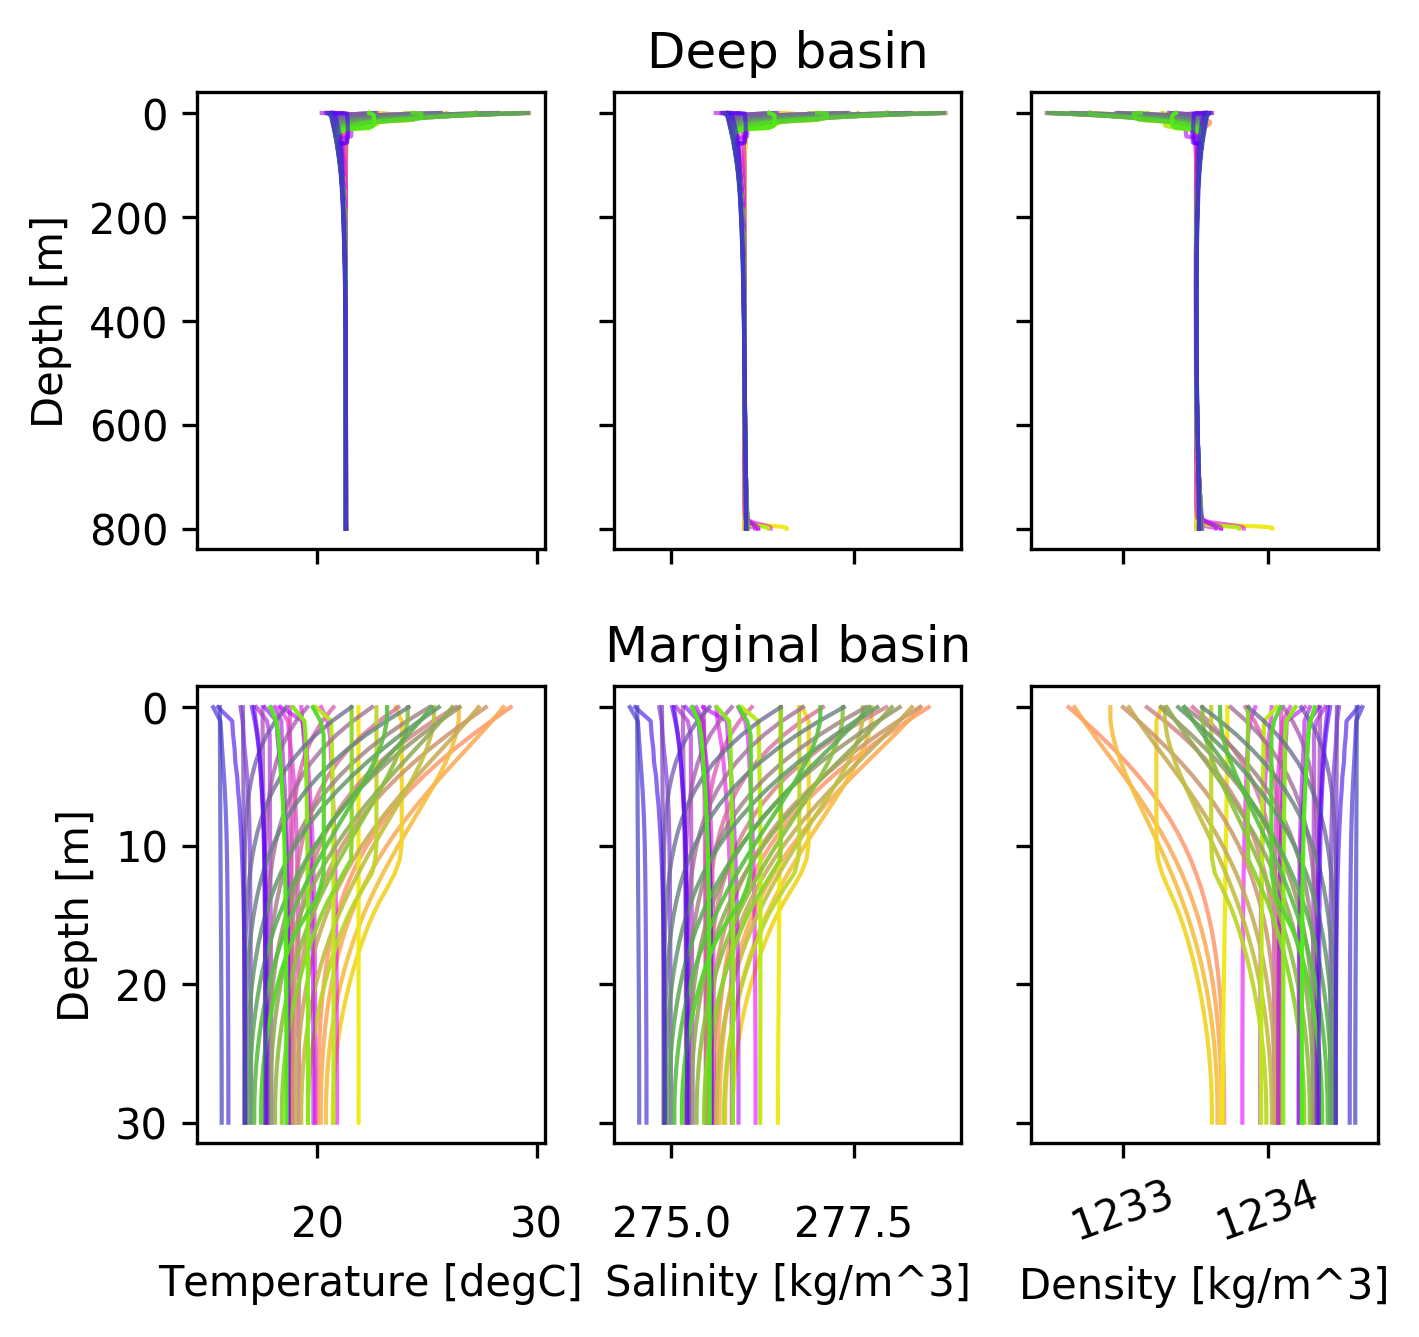
\includegraphics[width=\linewidth,keepaspectratio]{very_shallow_basin_success.png}
% \end{subfigure}\hfill
% %% subfig 2
% \begin{subfigure}[h]{0.20\textwidth}
% \centering
% 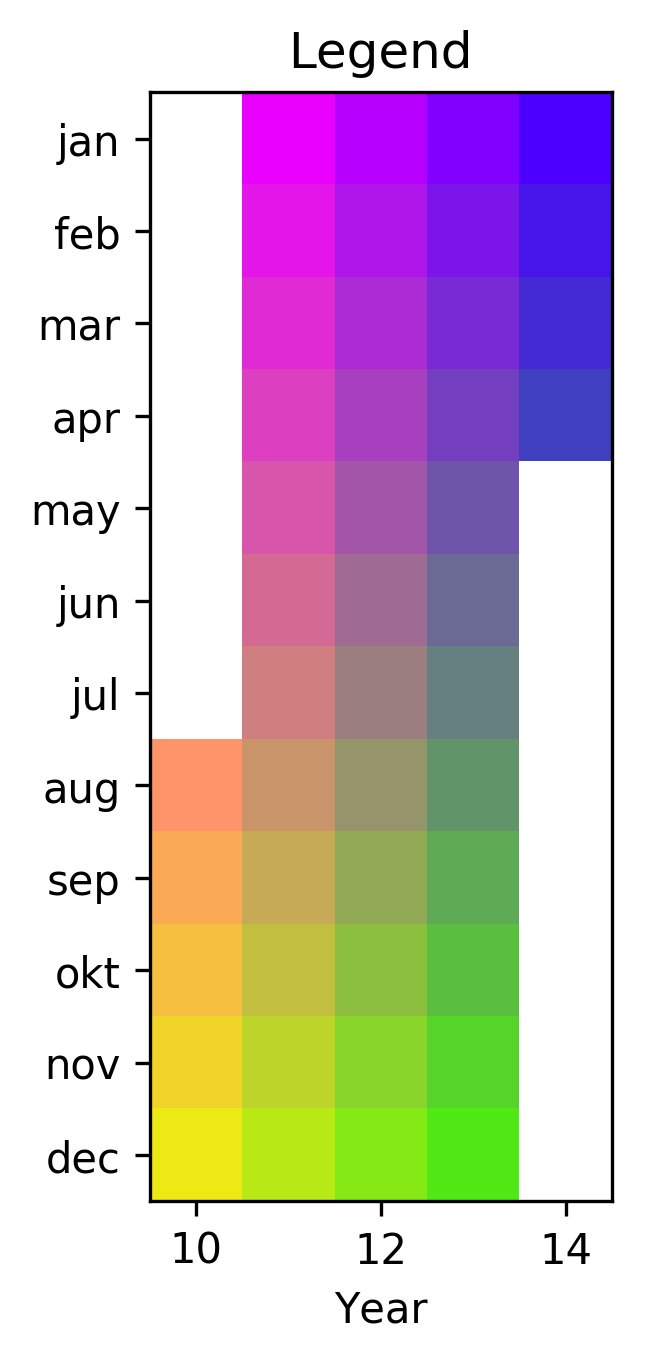
\includegraphics[width=\linewidth,keepaspectratio]{very_shallow_basin_success_Legend.png}
% \end{subfigure}\hfill
% \caption{Model run with a very shallow marginal basin.}
% \label{fig:Very shallow_bains_issue}
% \end{figure*}

% % % Fig with adv, shallow basin, grote uitslag
% % %-------------------
% \begin{figure*}
% %% subfig 1
% \begin{subfigure}[h]{0.8\textwidth}
% \centering
% 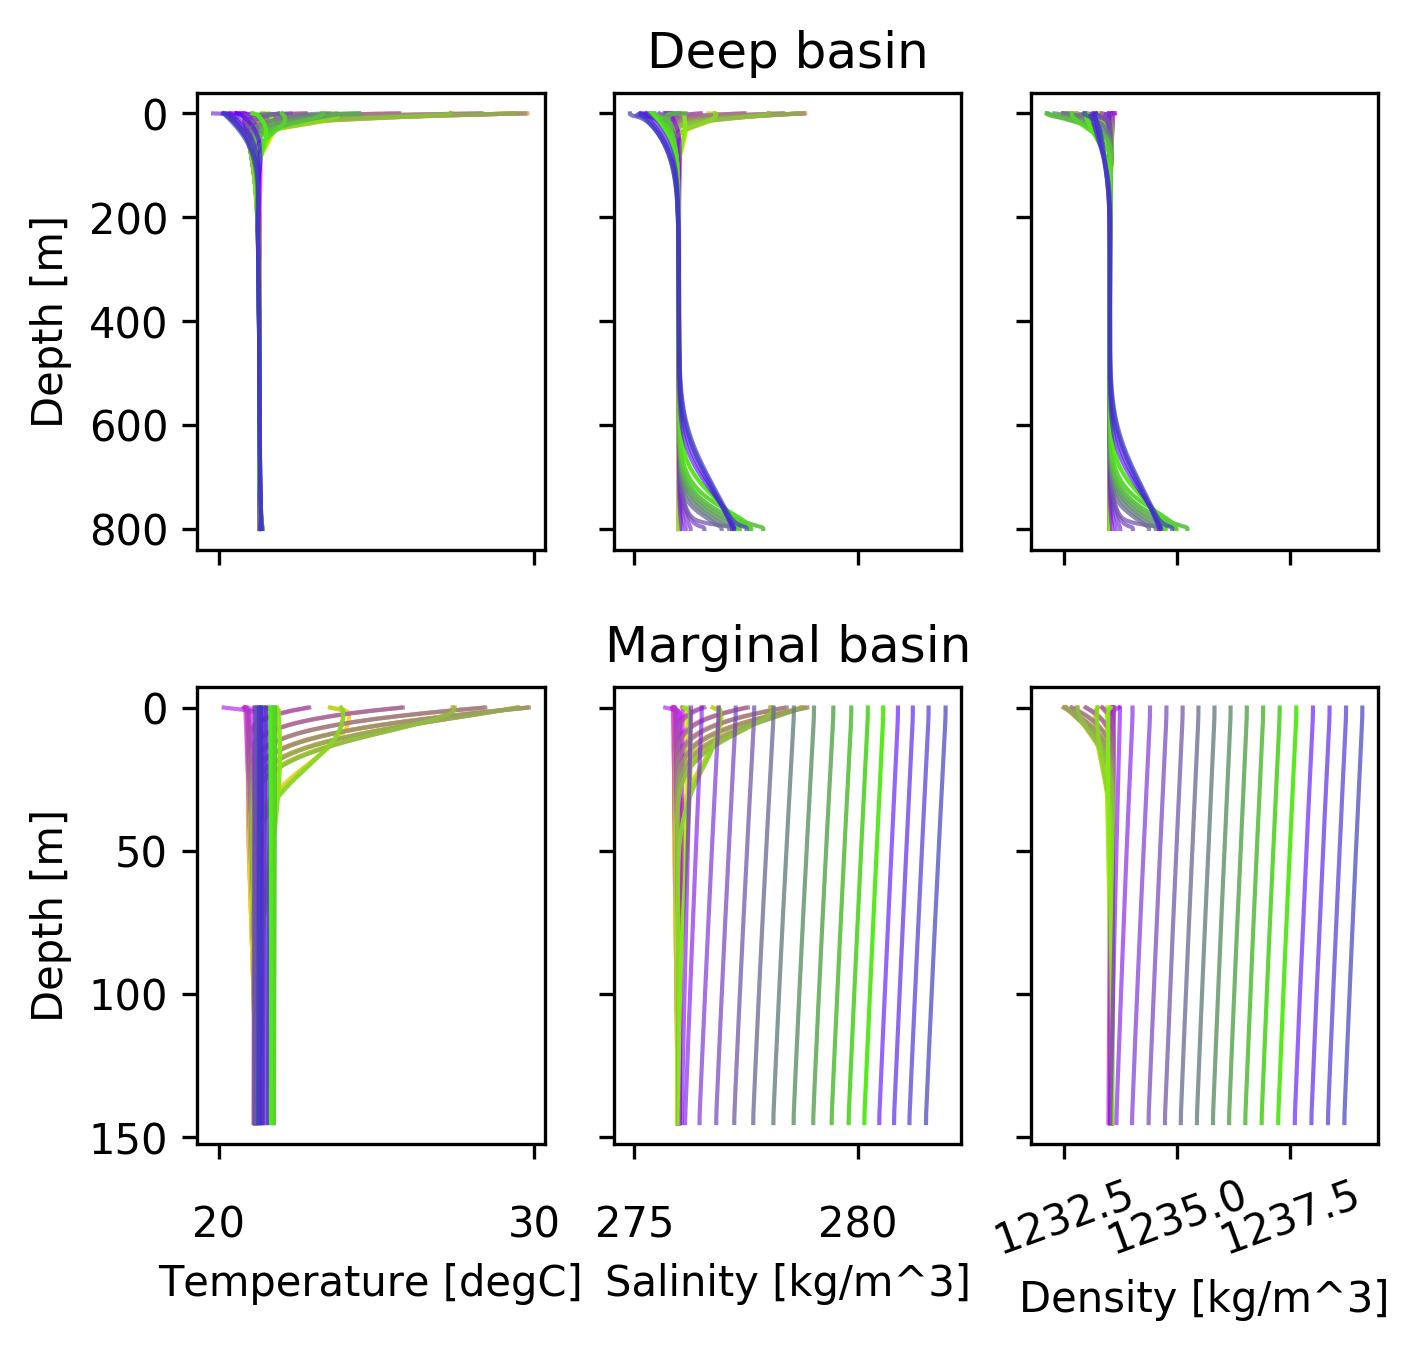
\includegraphics[width=\textwidth,keepaspectratio]{shallow_basin_with_saline_bot.png}
% \end{subfigure}\hfill
% %% subfig 2
% \begin{subfigure}[h]{0.20\textwidth}
% \centering
% 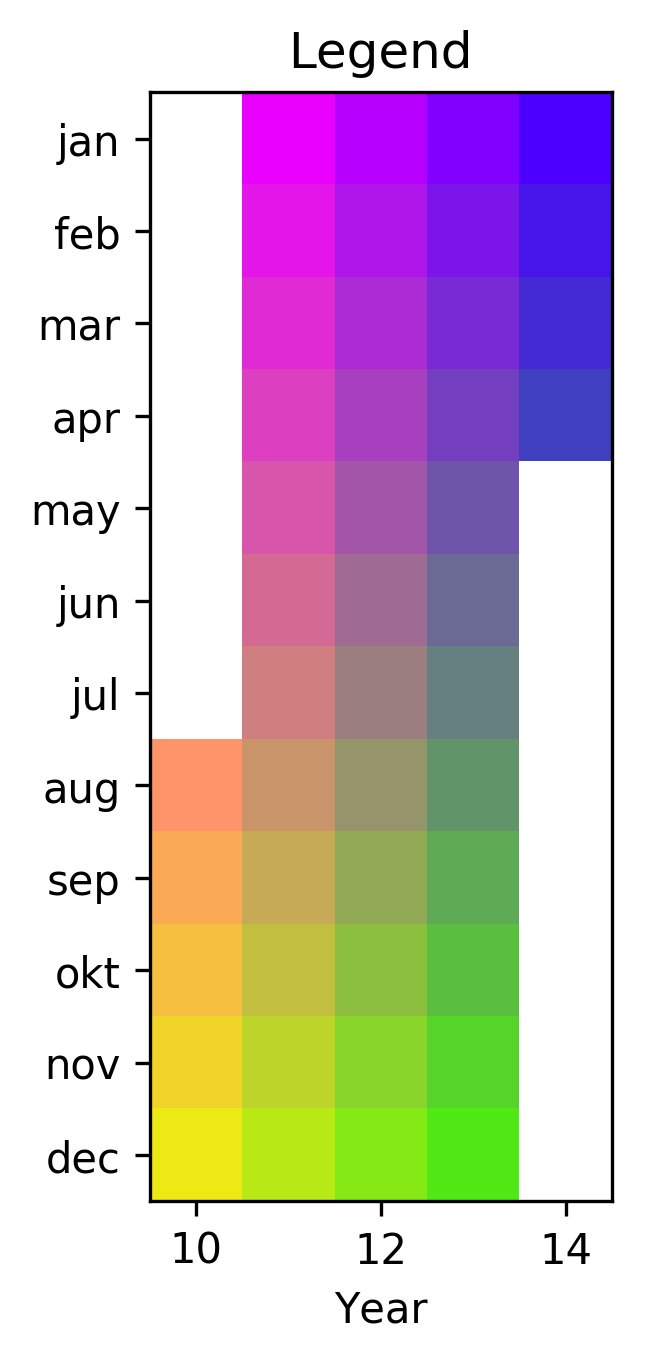
\includegraphics[width=1.0\textwidth,keepaspectratio]{shallow_basin_with_saline_bot_Legend.png}
% \end{subfigure}\hfill
% \caption{Model run with advection, a flow of 5e-5 Sv and a marginal basin depth of 145 metres.}
% \label{fig:with_adv_large_effect_145m}
% \end{figure*}

% \subsubsection{Background diffusivity}
% % % Fig with high background diff
% % %-------------------
% \begin{figure*}
% %% subfig 1
% \begin{subfigure}[h]{0.8\textwidth}
% \centering
% 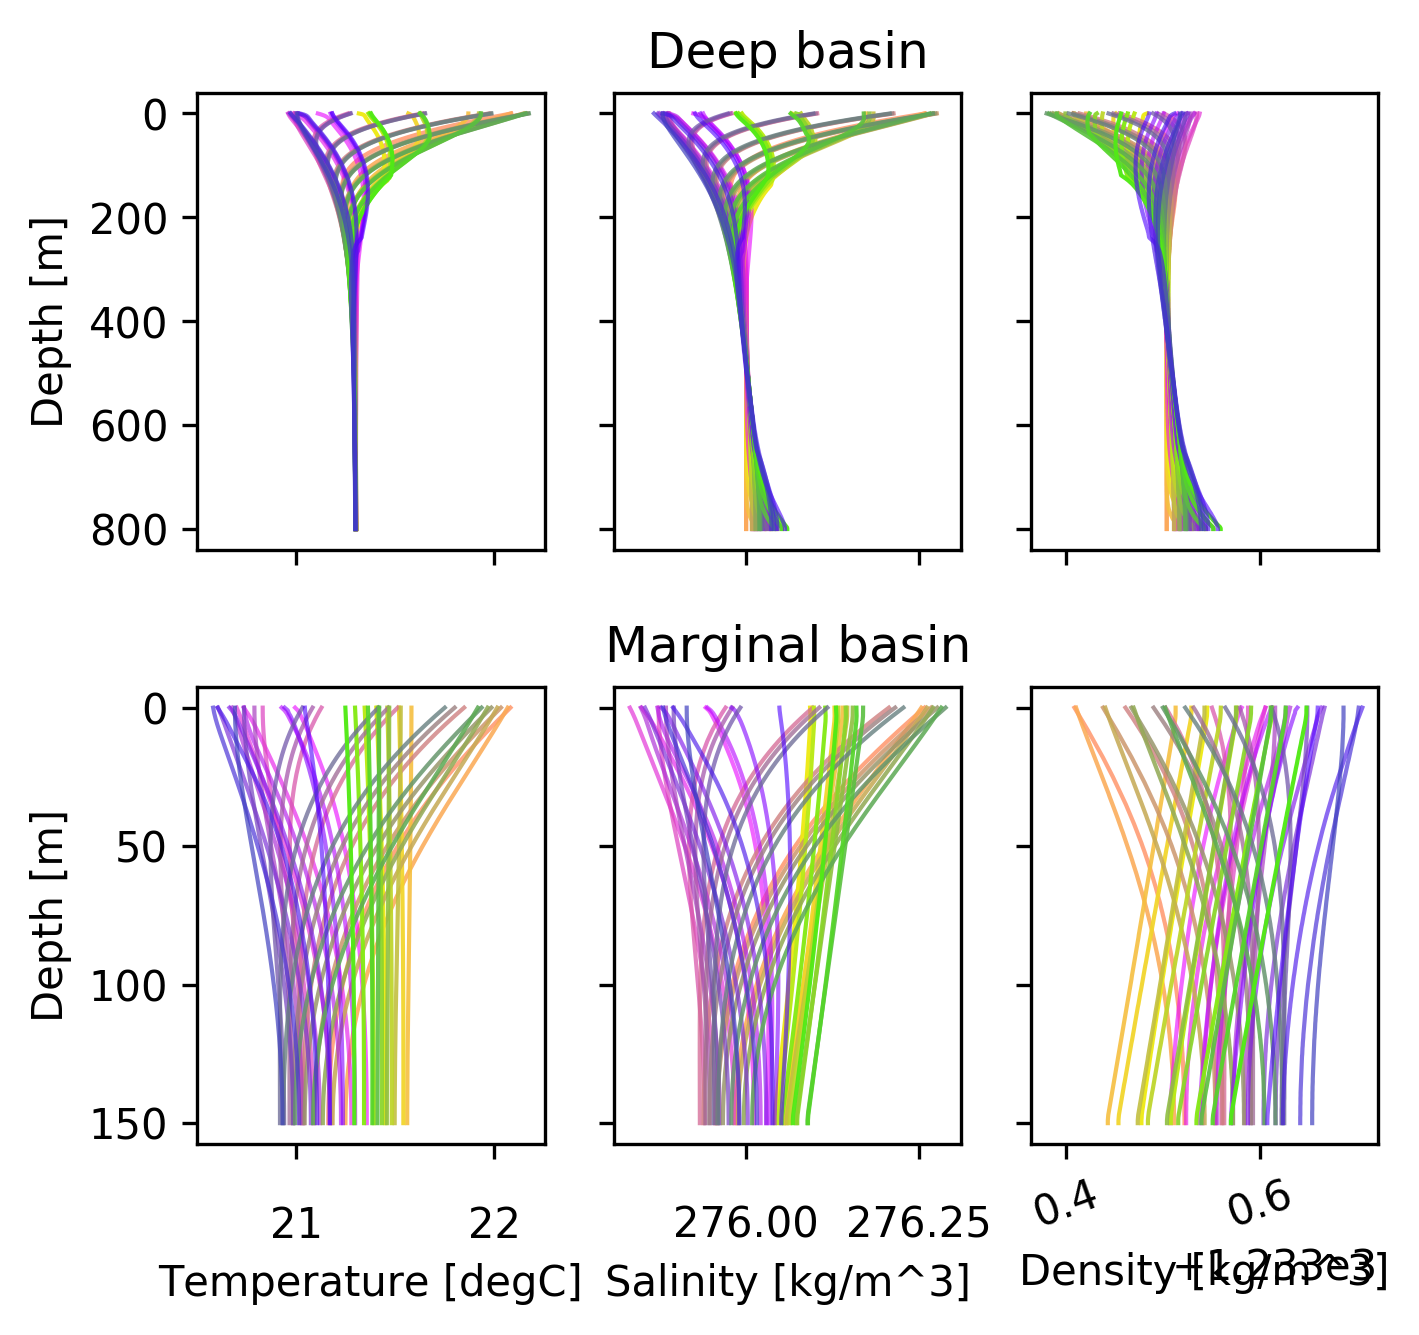
\includegraphics[width=\textwidth,keepaspectratio]{high_bg_diff_success.png}
% \end{subfigure}\hfill
% %% subfig 2
% \begin{subfigure}[h]{0.20\textwidth}
% \centering
% 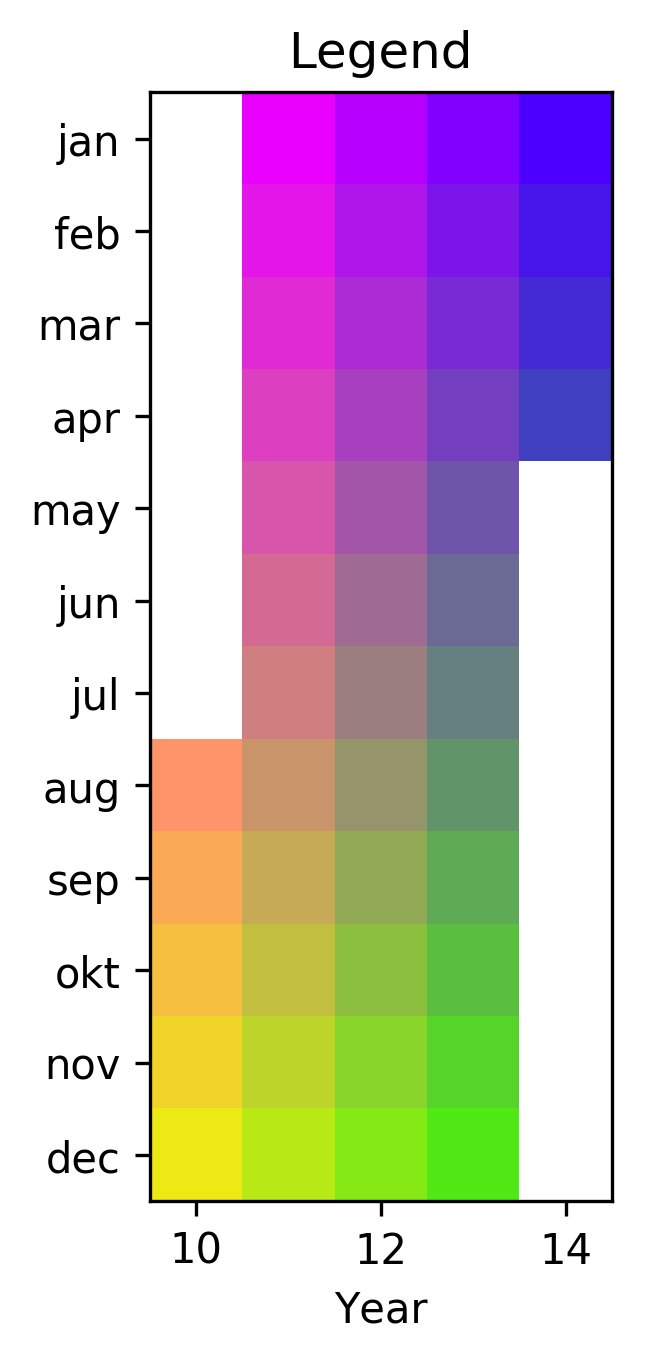
\includegraphics[width=1.0\textwidth,keepaspectratio]{high_bg_diff_succesLegend.png}
% \end{subfigure}\hfill
% \caption{Model run with advection, a flow of 1e-5 Sv and a marginal basin depth of 150 metres. The background diffusivity was increased, allowing surface processes to penetrate to greater depth}
% \label{fig:high_db_success}
% \end{figure*}

% \subsubsection{Net Evaporation}


% \subsubsection{Summer mixing}
% % % Fig with summer mixing, kleine uitslag
% % %-------------------
% \begin{figure*}
% %% subfig 1
% \begin{subfigure}[h]{0.8\textwidth}
% \centering
% 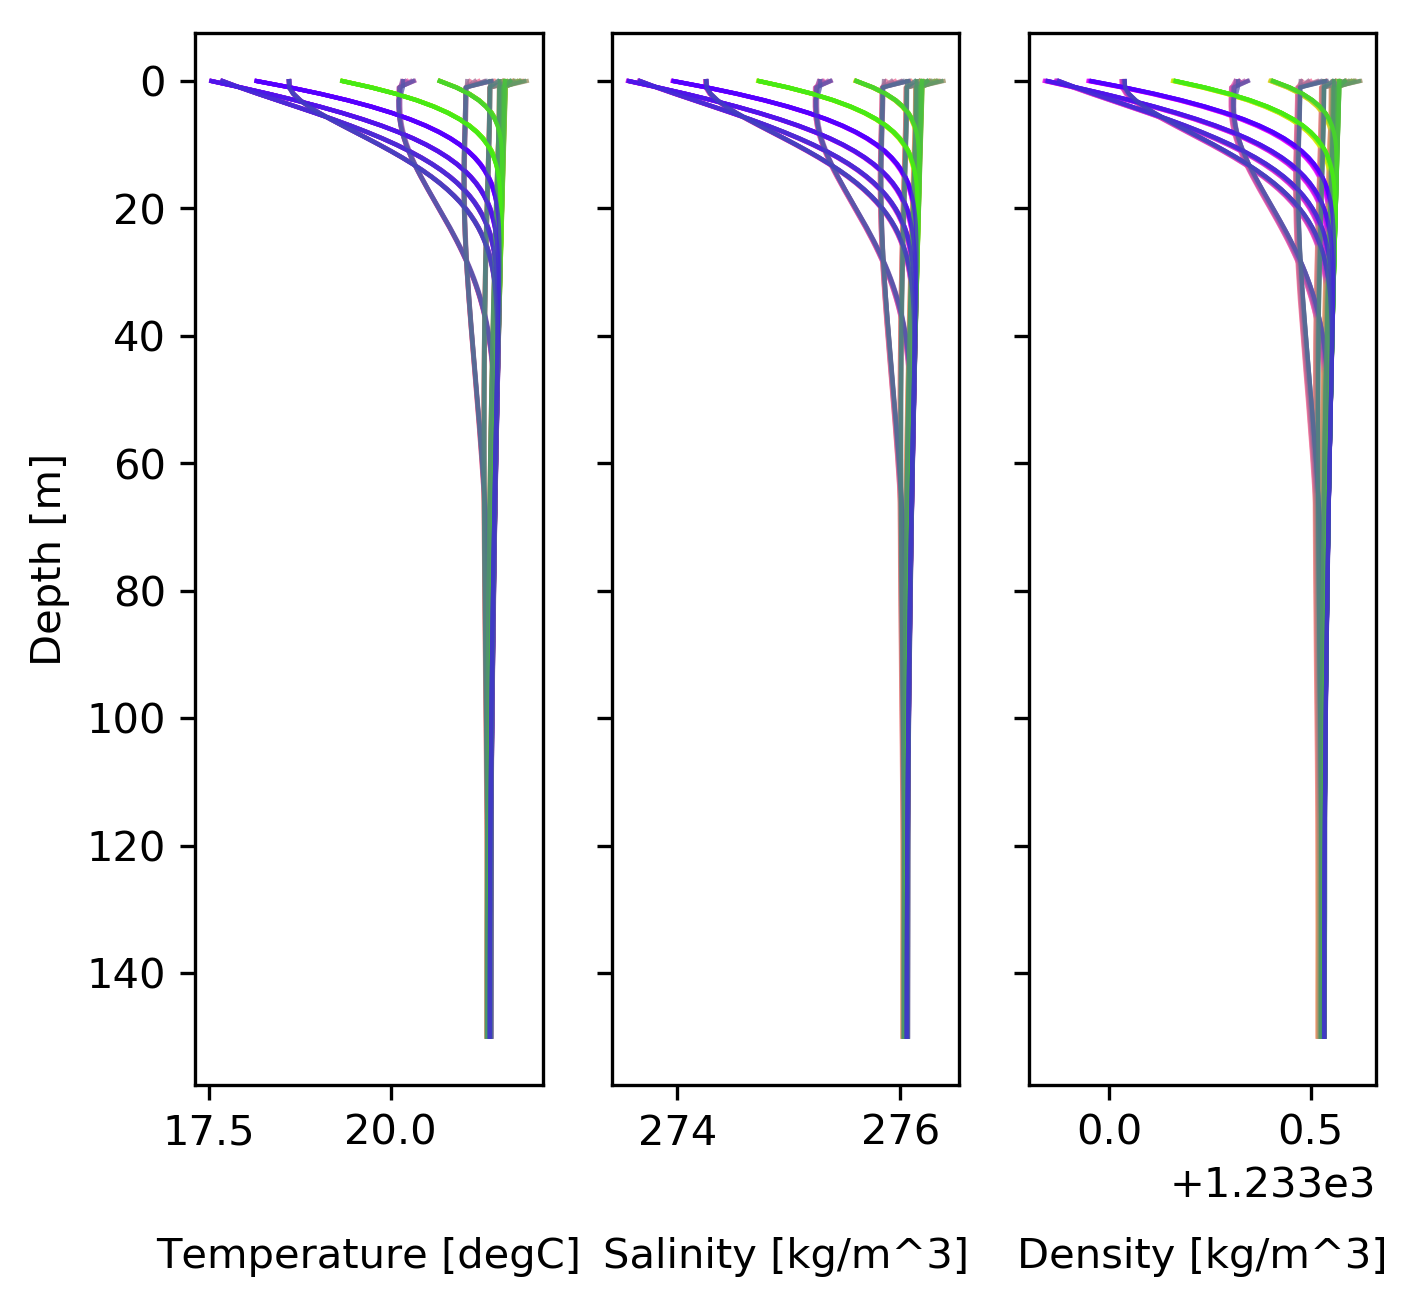
\includegraphics[width=\textwidth,keepaspectratio]{summer_mixing.png}
% \end{subfigure}\hfill
% %% subfig 2
% \begin{subfigure}[h]{0.20\textwidth}
% \centering
% 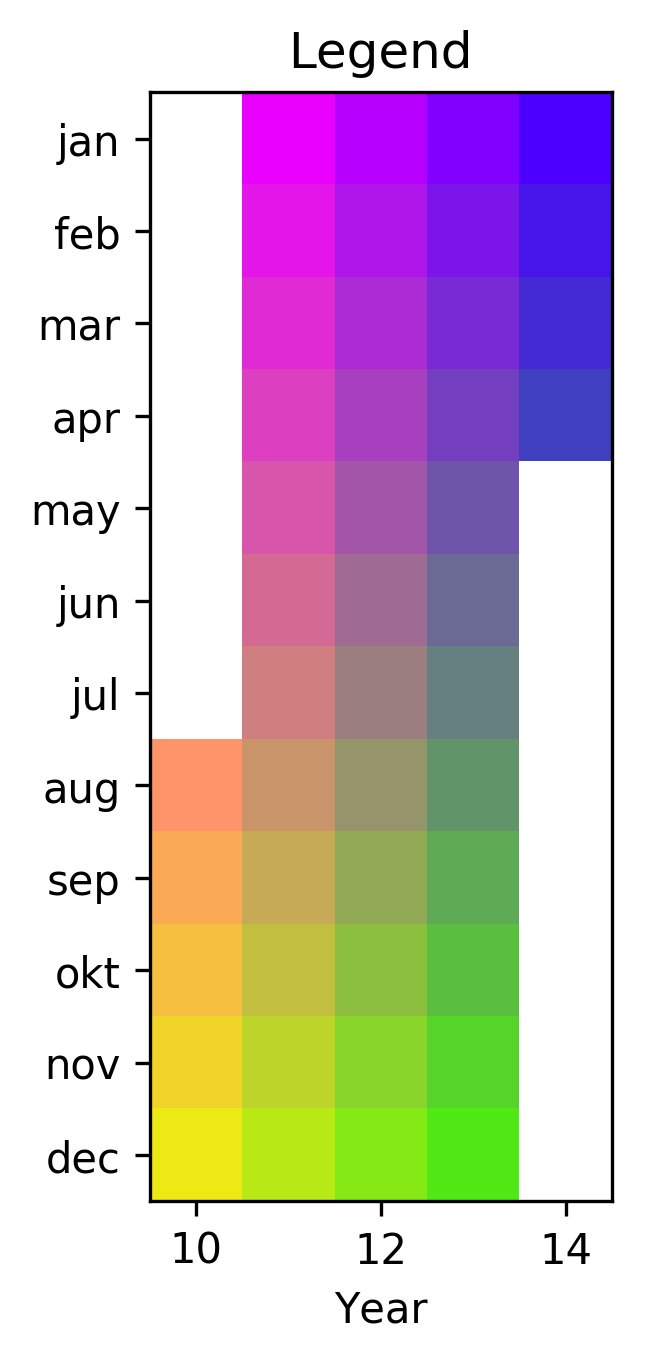
\includegraphics[width=1.0\textwidth,keepaspectratio]{summer_mixing_Legend.png}
% \end{subfigure}\hfill
% \caption{Model run with advection, a flow of 5e-5 Sv and a marginal basin depth of 100 metres. The evaporation amplitude was doubled, inducing mixing in summer.} \todo{run with same depth as the rest}
% \label{fig:with_adv_large_effect_145m}
% \end{figure*}

% \section{Discussion}
% \subsection{SpinUp period}
% During the spin-up period, the temperature, salinity and density profiles show a symmetrical overall shape of the plot (see figure~\ref{fig:SpinUp}). This shape follows from the perfectly sinusoidal cyclicity of the forcing that is centered around zero. Below about forty metres there is no influence of the forcing for the background diffusion is not quick enough to reach that depth within half a year, before the forcing is turned around. 

% \subsection{Influence of diffusivity on the density profile}
% \label{sect:diff_and_bcl}
% A lower diffusivity, as shown in the salinity in figure \ref{fig:SpinUp_dencity_balance_example} when compared to that of figure \ref{fig:SpinUp}, has two significant consequences. The first of these is the reduced depth to which the surface conditions can penetrate. The second is the inverse relation between the diffusivity and the forcing. The higher forcing on the salinity in figure \ref{fig:SpinUp_dencity_balance_example} results in a higher amplitude in the salinity values. This means that, during winter, the surface water is less saline then for example that in figure \ref{fig:SpinUp}, resulting in a stable density distribution during winter. Since this effect only penetrates the water column for the first few metres, deeper in the column the temperature has more impact and the inverse balance of the density curve as seen in figure \ref{fig:SpinUp} is restored. This can be deduced from the equation of state as well (equation \ref{eq:state}), where the density lowers in a given location if $\alpha T$ increases more rapidly then $\beta S$ or $\beta S$ decreases more more rapidly then $\alpha T$. The latter is the case in figure \ref{fig:SpinUp_dencity_balance_example}. If the amplitude of evaporation forcing is significantly higher then the amplitude of the heat flux forcing, the salinity of the water will control the density profile. If that is the case, and assuming there is no net evaporation, the surface water lacks the salinity to become dense enough during winter to become unstable, while the water becomes so dense during summer that the water column becomes unstable, despite its high temperature. \todo{investigate this when evap mean .ne. 0}

% \subsection{The transition period}
% \label{sect:Discussion_transition}
% Concerning the transition, as shown in figure~\ref{fig:Transition}, the mixing should start in April. This is namely the moment when convection is switched on, and the density in the top node is higher then the rest of the column. The mixing does however not occur until October, as read from figure~\ref{fig:Transition}. The cause of this is that the code begins the instability check by checking whether the top node is more dense then the one below it. Since, in April, year 10, the top node is as dense as the one below it, is considered stable. Even if the top twenty metres are more dense then the water below it. This situation generally only occurs during the transition, for the top nodes are always the first to move. The exception to this is a source-sink pulse, pulling salt from the bottom of the marginal basin, without directly affecting the water in the middle of the column. In order to have mixing in the bottom of the column to resupply salt to the bottom of the marginal basin and restore the density instability, a more rigorous check for instability is required, mentioned in section \ref{sect:stability_methods}. When checking the column for instability both from the top node down and from the bottom node up, the salt deprivation in the bottom of the marginal basin after flow is solved in this way. The artifact that arises during the transition period as shown in figure~\ref{fig:Transition} does however remain.
% The alternative method was to check each individual node for stability. This method solves both the artifact during the transition and the salt deprivation in the bottom of the marginal basin. In practice, the whole column check can take up to an order of magnitude longer to run. This is not only due to the increase in effort to check for the whole column, but mainly due to the limiting factors shown in equation~\ref{eq:FCTS_limits}, where the highest diffusivity in the column determines the size of the time step. A few scattered unstable nodes can therefore significantly impact the run time. 
% An unforeseen issue arises when the whole column check is used, where certain scenarios result in an ever increasing salt content of both columns. An example of this is shown in appendix \todo{ref to app}. A scenario run with the input parameters as shown in appendix \todo{ref to input data in app} and a marginal basin depth of 150m will produce a stable outcome, but a scenario with 149m marginal basin depth results in instability like that shown in appendix \todo{ref to app}. This indicates that there is some stability threshold for the code, but this has not been narrowed down yet. When performing a column stability check from the top down and bottom up, this scenario can also occur, but for this to happen the marginal basin would need to be a mere 25m or so, with high $U_{lat}$.

% \todo{separate transition and whole column convection} \todo{talk about transition with whole col check}

% \subsection{Source sink and advection}
% \label{sect:SS_&_adv}
% The exchange between the marginal basin and the deep basin, shown in figure \ref{fig:no_adv}, lowers the total amount of salt in the marginal basin, for the water that flowed out is more saline then the water that flowed in. Then, when mixing occurs during each consecutive summer in the marginal basin, saline water is resupplied to the bottom waters. In the deep basin, the saline water body is stable but is shrinking due to diffusion. As the deep saline water is largely diffused away, a new dense plume from the marginal basin may arrive to repeat the process. 
% Since there is no advection in the run shown in figure \ref{fig:no_adv}, the flow cycle is broken which is realistically impossible for this would create space problems.
% The model run shown in figure \ref{fig:with_adv_geen_uitslag} was initialized with the same conditions as that in shown \ref{fig:no_adv} but during the periods of exchange, advection was allowed. Evidently, advection completely removed the effect of the source-sink term. Any water that arrived in the deep basin was directly being advected up thus not allowing for a dense water body at the bottom of the deep basin. In order to investigate how the model handles these advection situations, the model was run with a flow of 40 Sv. This amount of volume is in no way realistic but makes it easier to investigate the workings of the model. Figure \ref{fig:ww_large_effect_legend} shows an annotated plot of this model run. This figure shows that right after the initiation of flow (1), the deep basin is fully stable with denser than average waters at the bottom and the least dense water at the top. Most of any negative density anomaly at the base of the marginal basin is directly resupplied by mixing. From the initiation of flow (1) until the next mixing during winter (3), the salt anomalies dissipate slowly due to diffusion (2). When the columns mix in winter, the bottom waters of the deep column are unaffected due to their stable state. During this mixing period, some salt is resupplied to the bottom of the basin, leading to a small jump in the density plot. 
% Aside form the large amount of flow required for this effect to be visible, an issue becomes apparent when analyzing figure \ref{fig:ww_large_effect_legend}. In the conceptual model, the water does not increase its salinity as it flows between the basins. However, due to the technical choice of imitating the flow with the source-sink term, combined with this large flow, the bottom waters of the deep basin become significantly more saline then the bottom of the marginal basin ever was. In order to obtain a dense saline brine at the bottom of the deep basin, the bottom of the marginal basin clearly needs to be significantly more saline then is achieved with the parameters used in the runs shown so far \todo{list these in app}. This could be done by increasing the total amount of salt in the marginal basin through net evaporation or by allowing for faster transport of salt to the bottom of the marginal basin. The latter can be achieved by decreasing the basin depth or increasing the amount of diffusion during mixing. A combination of these is likely required to achieve the sought effect. These factors will be discussed in section \ref{sect:imprtant_parameters}.

% \subsection{Important parameters}
% \label{sect:imprtant_parameters}

% \subsubsection{Marginal basin depth}
% \label{sect:shallow_basin_issue}
% In shallow basins, the forcing is dominant in a large part of the column when compared to deeper basins, which is fully expected for both columns are subject to the same diffusivity. Figure \ref{fig:Very shallow_bains_issue} however, shows an unforeseen decrease in both the temperature and salinity. Since the decrease in temperature is faster then that of the salinity, the density keeps increasing. This decrease in salinity and temperature is a consequence of the low amount of total salt and heat stored in the shallow column. Changes in salt content and total heat now have a pronounced effect. In this case, the change in total salt and heat content can be due to two factors. The first option is the flow between columns where the marginal basin loses more then it gains, as discussed in section \ref{sect:SS_&_adv}. The second option is a net loss of salt and heat during mixing in winters. Since the diffusion is set higher then    %%CONTINUE HERE about fig \ref{fig:Very shallow_bains_issue}  DOES THIS ONLY HAPPEN WITH HIGH ADV??

% Figure \ref{fig:with_adv_large_effect_145m} was run with a marginal basin that is only slightly more shallow then that of figure \ref{fig:with_adv_geen_uitslag} and has a significantly lower connective flow. 
% \subsubsection{Background diffusivity}

% \subsubsection{Net evaporation}





\subsubsection{Extend of the salt brine}
It was suggested by \cite{garcia2018geochemical} that the brine would extend roughly from the base of the marginal basin to the bottom of the deep basin. In the conceptual box model this would also make sense, for dense water in the marginal basin may as well replace water slightly higher in the deep basin if the bottom water of the deep basin is too dense to be replaced with the dense water from the marginal basin. This could happen as long as that water is below the base of the marginal basin. This has not been implemented in the model, but may be worth investigating in further research.

\subsubsection{Buoyancy}
This model deals with instability by mixing the unstable columns, for this is the observed process in the Dead Sea. This model does not take into account any other type of gravity interaction with the water, except for the assumption that dense water from the bottom of the marginal basin flows to the bottom of the deep basin if the density allows for it, which is hard coded into the model. When a dense water mass resides below the surface and is considered unstable, the diffusivity is increased drastically to imitate mixing, meaning that the dense mass is moved both up and down, where the water is less dense. Restricted mixing of saline water bodies with the environment and the possibility of this dense water body to sink due to buoyancy forces rather then be diffused up as well, is not considered in this model.

\section{Conclusion}
If the MSC evaporite deposits originated from a deep sea, a dense brine may have existed at the bottom of the basin from where the evaporites precipitated. This deep brine may have formed as a result of the shallow marginal basins that acted as large evaporative pools where water may have flowed in at the top and out at the bottom. This flow could have been driven by density differences between the bottom waters of the marginal basin and the water in the deep basin that resides below the depth of the marginal basin. Since small differences in salinity are quickly re-distributed due to diffusion of salt, the difference in salinity would either need to be substantial or regularly supplemented. Two methods of achieving very saline bottom waters in the marginal basin were investigated. 

The first is net evaporation averaged out over the year. If the net evaporation per unit of surface area does not differ between the deep and marginal basins, the effect is larger in the marginal basins due to their smaller volume. In periods where the water column is mixing, salt is brought to the bottom of the marginal basin from where it may flow into the deep basin. 

The second method to achieve a similar effect, where no net evaporation is required, is when the effects of the increase in salinity of the basins during summer are able to reach the bottom of the marginal basin. One scenario in which this can happen is in a basin that is shallow enough for the effects to reach the bottom before summer is over. In our numerical experiment this scenario was capable of producing a small increase in salinity at the bottom of the deep basin, with a marginal basin depth of a mere sixty metres. Increasing the background diffusivity of salt is a second way to have the seasonal effects penetrate deeper into the water column. This scenario also succeeded in creating a slightly more saline deep water. The combined effect of a shallow marginal basin with high background diffusion was capable of producing a significant salt excess at the bottom of the deep basin, though this scenario is still more limited then a scenario involving net evaporation. 
A final scenario in which the saline summer waters can reach the bottom is through mixing in summer rather then in winter. While this scenario is not the current condition of the Dead Sea, this scenario can occur when the increase in density of the surface water in summer due to high evaporation is larger then the decreasing effect heating has on its density.

This research is a first order approximation of the scenario and detailed scenarios of the climate and flow patterns during the MSC are beyond the scope of this research. Nevertheless, this research does indicate that it may be possible to create deep saline brines through high evaporation in marginal basins.


% \begin{figure*} 
% \centering
% \includegraphics[width=0.8\textwidth,keepaspectratio]{}
% \caption{}
% \label{fig:}
% \end{figure*}

% \begin{figure*}
% %% subfig 1
% \begin{subfigure}[b]{0.48\textwidth}
% \centering
% \includegraphics[width=\textwidth,keepaspectratio]{}
% \caption{}
% \label{fig:}
% \end{subfigure}\hfill
% %% subfig 2
% \begin{subfigure}[b]{0.48\textwidth}
% \centering
% \includegraphics[width=\textwidth,keepaspectratio]{}
% \caption{}
% \label{fig:}
% \end{subfigure}\hfill
% \caption{}
% \label{fig}
% \end{figure*}

\clearpage
\pagebreak
\bibliography{bibliography}

\clearpage
\pagebreak
\begin{appendices}
\section{Standard parameters}
\label{app:standard_parameters}
\begin{table}[H]
\begin{tabular}{lll}
\textbf{Parameter}          &\textbf{Unit}                  & \textbf{Value} \\   
Depth\_Main\_basin          &{[}m{]}                        & 800       \\
Depth\_sec.\_basin          &{[}m{]}                        & 150       \\
tmax                        &{[}years{]}                    & 20            \\
Cp                          &{[}J/K{]}                      & 4.e3      \\
dx                          &{[}m{]}                        & 1         \\
pb                          &                               & -5.1      \\
pc                          &                               & -2.0      \\
tau                         &                               & 86400     \\
Tbot                        &{[}$^{\circ}$C{]}              & 21.3      \\
Sbot                        &{[}$kg$ $m^{-3}${]}            & 276       \\
flowdepth                   &{[}m{]}                        & 5         \\
strait\_depth               &{[}m{]}                        & 500       \\
strait\_width               &{[}m{]}                        & 10000     \\
U\_lat                      &{[}m/s{]}                      & 0.0000020 \\
width\_basin1               &{[}m{]}                        & 70000     \\
width\_basin2               &{[}m{]}                        & 70000     \\
length\_basin1              &{[}m{]}                        & 100000    \\
length-basin2               &{[}m{]}                        & 10000     \\
Salt\_diff\_amplifier       &                               & 1         \\
Temp\_diff\_amplifier       &                               & 1         \\
evaporation\_amplifier1     &                               & 0.3       \\
evaporation\_amplifier2     &                               & 0.3       \\
mean\_evap\_rate            &{[}$kg$ $m^{-3}s^{-1}${]}      & 0         \\
Whole\_col\_instab\_check\  &  boolean                      & True      \\
Source\_sink                &  boolean                      & True      \\
Advection                   &  boolean                      & True   
\end{tabular}
\end{table}



% \section{Figures}
% \subsection{Years 11-15 with diffusion and advection only}
% \label{App:years_11-15_conv_only}
% \vspace{2mm} %%Vspace
% %Figure
% \begin{figure*} 
% \centering
% 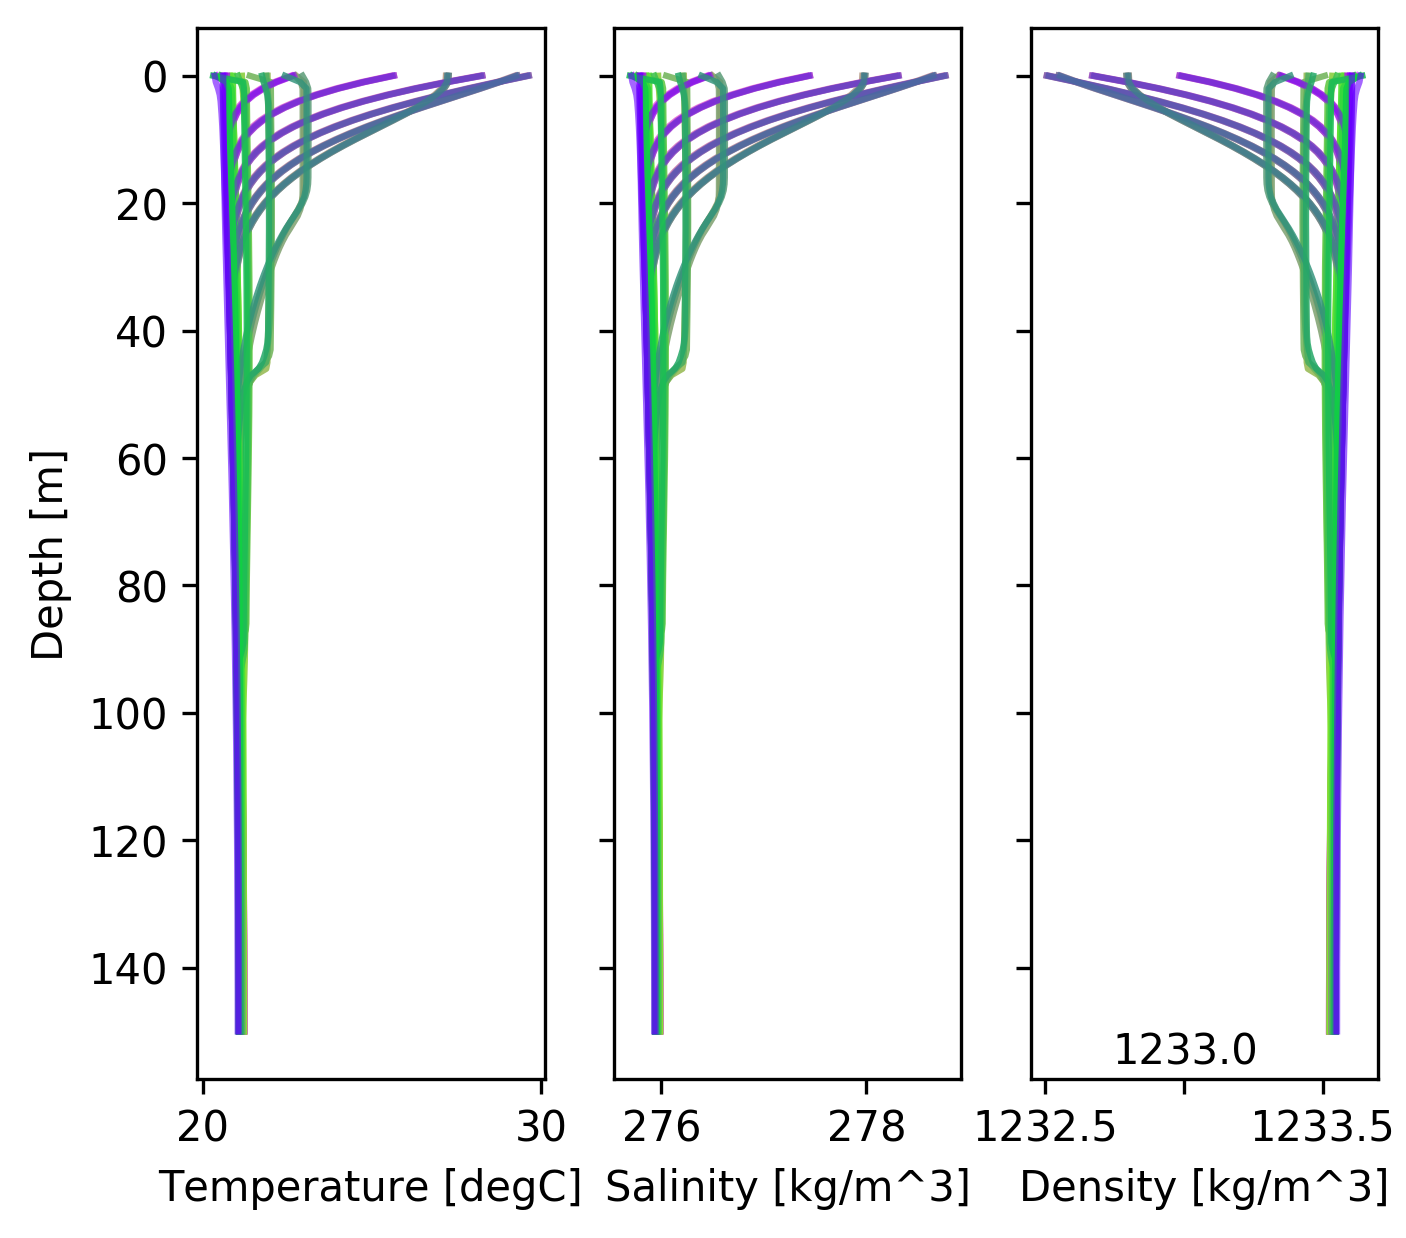
\includegraphics[width=0.80\textwidth,keepaspectratio]{conv_only_years11-15.png}
% % \caption{ranging from year 11-15}
% \label{App:fig:legend_11-15}
% \end{figure*}
% 
% Legend
% \vspace{2mm} %%Vspace
% \begin{figure*} 
% \centering
% \caption*{Legend}
% \vspace{-3mm}  %%vspace
% 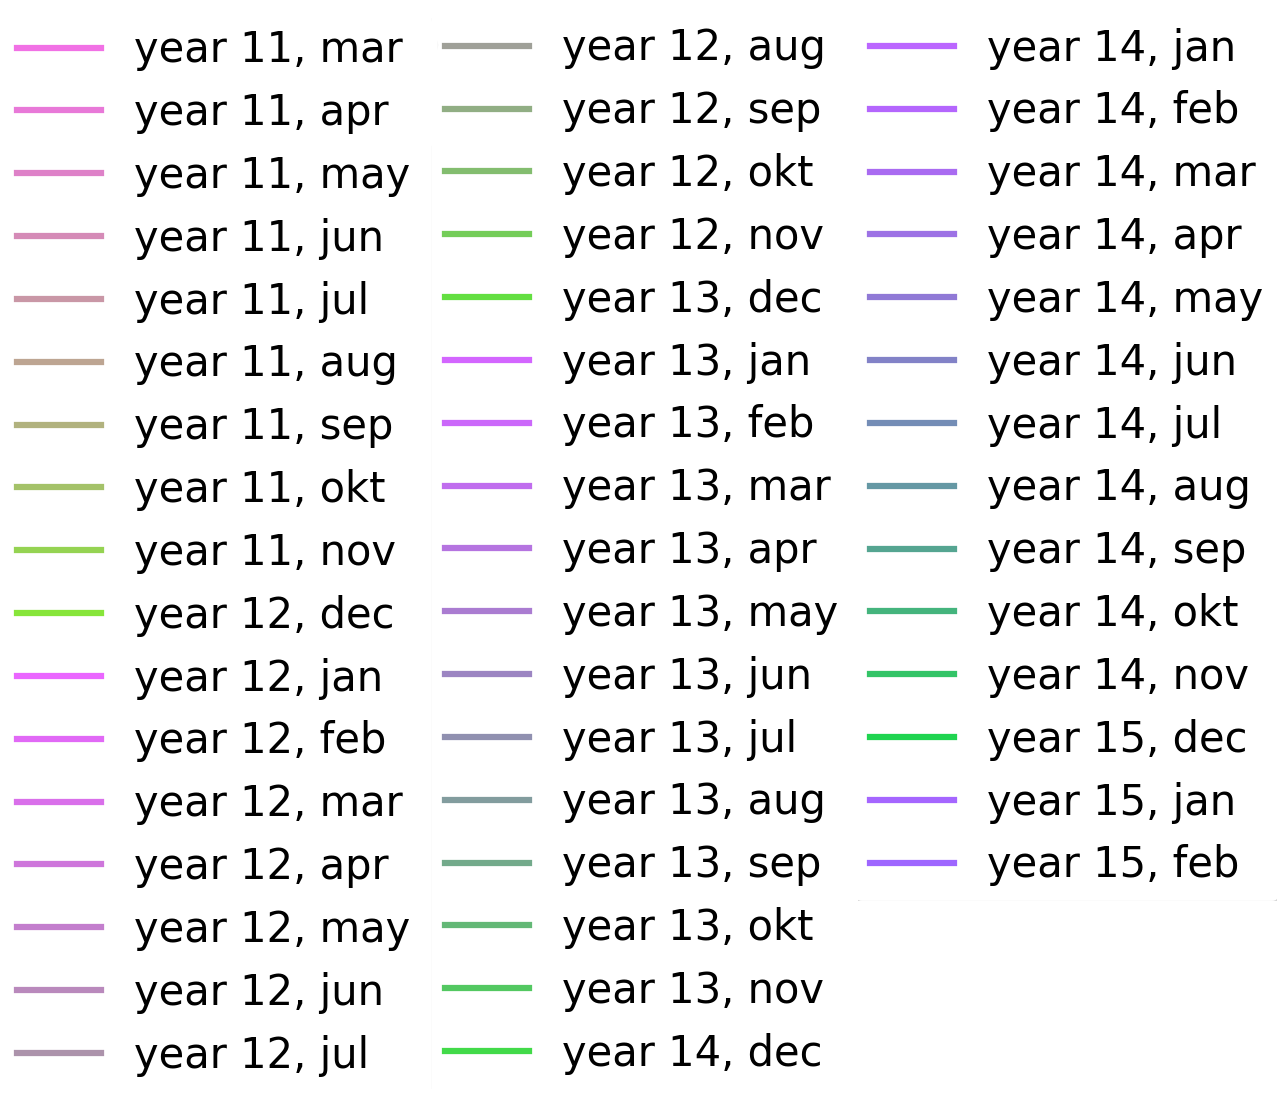
\includegraphics[width=0.65\textwidth,keepaspectratio]{years11-15_legend.png}
% \label{App:fig:legend_11-15}
% \end{figure*}


\end{appendices}

\end{document}
